\chapter{Results and Conclusions}
\label{ch:res}
\textcolor{red}{This sounds like it is the last Chapter. Is it? The hierarchical model is neither a 'Result' nor a 'Conclusion' so why is it in this Chapter? Something is very wrong with your structure.
	This appears to contain Modelling and Numerical Experiments - -and those should be separate Chapters. }
In this chapter, we use the forward model to generate some data given an underlying ground truth and then guide the reader through the process of setting up a Bayesian framework and ultimately obtaining the posterior distributions of hyper-parameters and parameters of interest, such as ozone concentration or pressure and temperature profiles.
We use DAGs to visualise hierarchical and correlational structures of a Bayesian model, establish a choice of prior distributions within our Bayesian model and formulate the posterior distributions.
All programming and analysis is done in Python, and the reported computation times correspond to a MacBook Pro from 2019 with a 2.4 GHz quad-core Intel Core i5 processor.

Based on the linear forward model $\bm{A}_L$, we characterise the marginal posterior for ozone and compare that to the TT approximation.
Then we calculate the mean and the covariance matrix of the full posterior for ozone, which we use to generate posterior ozone samples and according to those find an affine map to approximate the non-linear forward model $\bm{A}(\bm{x}) \approx \bm{M} \bm{A}_{L} \bm{x}$ (see Sec.~\ref{sec:affineMap}).
In Sec.~\ref{sec:ComparReg}, we repeat the MTC scheme to provide a posterior distribution of ozone based on the approximate forward model and compare it to a regularisation approach and a ground truth.

In Sec~\ref{sec:FullBay}, we extend the hierarchical Bayesian model and MTC scheme to jointly provide posterior distributions of ozone, temperature and pressure.
Here, we elaborate on some aspects of prior modelling and on our findings when using a TT to approximate the higher-dimensional marginal posterior.

\clearpage

\section{Simulate Data based on a Ground Truth}
As the ground truth for our methodology, we consider an ozone profile at distinct pressure values generated from some data~\cite{MLSdata} of the MLS on the Aura satellite within the Antarctic region.
This ozone profile has a peak in the middle atmosphere and a second peak at higher altitudes, see Fig.~\ref{fig:O3Samp}, which seems to be a typical nighttime profile~\cite{Lee2020NightOzone}.

We recursively relate pressure $p$ to geometric height $h$ with the hydrostatic equilibrium equation
\begin{align}
	\frac{\text{d}p}{p} = \frac{- g M}{R^* T} \text{d} h \, ,\label{eq:hydr}
\end{align}
starting with a pressure of $1013.25$hPa at sea level.
The acceleration due to gravity
\begin{align}
	g = g_0 \Bigg( \frac{r_0}{r_0 + h} \Bigg) \, ,
\end{align}
where the polar radius of the earth is $r_0 \approx 6356 \, \text{km}$, the gravitation at sea level is $g_0 \approx 9.81 \text{m}/\text{s}^2$, $R^* = 8.31432 \times 10^{-3} \text{Nm} / \text{kmol} / \text{K}$ and the mean molecular weight of the air is $M = 28.97 \text{kg/kmol}$~\cite{atmosphere1976us}.
This holds up to a geometric height of $86$km, where we ignore a $0.04\%$ non-linear change in $M$ from $80$km to $86$km.

Following \cite{atmosphere1976us} we form the temperature function
\begin{equation}
	\label{eq:tempFunc}
	T(h) = \adjustbox{max width=0.825\textwidth}{$\begin{dcases*}
			T_0 &, \text{$h  = 0$}\\
			T_0 + a_0 h   &, \text{$0 \leq h < h_{T,1}$}\\
			T_0 + a_0 h_{T,1} &, \text{$h_{T,1} \leq  h < h_{T,2}$}\\
			T_0 + a_0 h_{T,1} + a_1 (h_{T,2}   - h_{T,1})  + a_2 (h   - h_{T,2})  &, \text{$h_{T,2} \leq h < h_{T,3}$}\\
			T_0 + a_0 h_{T,1} + a_1 (h_{T,2}   - h_{T,1})   & \\
			\hphantom{{} T_0 } + a_2 (h_{T,3}   - h_{T,2}) + a_3 (h   - h_{T,3}) &, \text{$h_{T,3} \leq h < h_{T,4}$}\\
			T_0 + a_0 h_{T,1} + a_1 (h_{T,2}   - h_{T,1})  & \\
			\hphantom{{} T_0 }+ a_2 (h_{T,3}   - h_{T,2})  + a_3 (h_{T,4}   - h_{T,3}) + a_4 (h   - h_{T,4}) &, \text{$h_{T,4} \leq h < h_{T,5}$}\\
			T_0 + a_0 h_{T,1} + a_1 (h_{T,2}   - h_{T,1})   & \\
			\hphantom{{} T_0 } + a_2 (h_{T,3}   - h_{T,2}) + a_3 (h_{T,4}   - h_{T,3}) + a_4 (h_{T,5}   - h_{T,4})& \\
			\hphantom{{} T_0 }  + a_5 (h   - h_{T,5}) &, \text{$h_{T,5} \leq h < h_{T,6}$}\\
			T_0 + a_0 h_{T,1} + a_1 (h_{T,2}   - h_{T,1})    &\\
			\hphantom{{} T_0}  + a_2 (h_{T,3}   - h_{T,2}) + a_3 (h_{T,4}   - h_{T,3}) + a_4 (h_{T,5}   - h_{T,4}) &\\ 
			\hphantom{{} T_0} + a_5 (h_{T,6}   - h_{T,5}) + a_6 (h   - h_{T,6})   &, \text{$h_{T,6} \leq h \lesssim  86$}
		\end{dcases*}$}\\
\end{equation}
with gradient and height values provided by~\cite{atmosphere1976us} (see Tab.~\ref{tab:tempGrad}) which acts as the ground truth temperature profile (see Fig.~\ref{fig:PriorTemp}).
\begin{table}
	\centering
	\begin{tabular}{ |c||c|c|  }
		\hline
		subscript $i$ & geometric height $h_{T,i}$ in km&gradient $a_i$\\
		\hhline{|=||=|=|}
		0& 0 & -6.5\\
		1& 11 & 0\\
		2& 20.1& 1\\
		3& 32.2& 2.8\\
		4& 47.4& 0\\
		5& 51.4& -2.8\\
		6& 71.8& -2\\
		\hline
	\end{tabular}
\caption[Height depending temperature gradients]{Definition of height depending temperature gradients.}
\label{tab:tempGrad}
\end{table}

Then we can compute a data vector $\bm{y} = \bm{A}(\bm{x}) + \bm{\eta} $, with $m = 30$ measurements determined by the satellite pointing accuracy of $175\text{arc sec}$ (see case 5 in Fig.~\ref{fig:TangHCases}), according to the RTE as in Eq.~\ref{eq:RTE} and Eq.~\ref{eq:absRTE} using the trapezoidal integration rule.
We assume an atmosphere between $h_{L,1}=7$km and $h_{L,n} = 83.3$km with $n = 45$ equidistant layers (see Fig.~\ref{fig:LIMB}).
The height value $h_{L,i}$ for each layer $i = 1,\dots, n$ is defined by the pressure values from~\cite{MLSdata} and the hydrostatic equilibrium equation, see Eq.~\ref{eq:hydr}.
We target ozone at a frequency of 235.71GHz, which lies within the region where the MLS observes ozone~\cite{livesey2008ozonecarbonmono, waters2006earth}.
The corresponding wave number is $\nu = 7.86\text{cm}^{-1}$.
We calculate the absorption constant $k(\nu,T)$ as in Eq.~\ref{eq:absRTE}, following the high resolution transmission (HITRAN) database~\cite{gordon2022hitran2020}, which provides the line intensity $L(\nu,T_{\text{ref}})$ for the isotopologue $\prescript{16}{}{\text{O}}_3$ with the AFGL Code 666.
%This gives us a non-linear forward model matrix $\bm{A}_{NL} = \bm{A}(\bm{x}, \bm{p}, \bm{T}) \in \mathbb{R}^{m \times n}$, where $\bm{x}\in \mathbb{R}^{n}$ is vector related to the ozone VMR, $\bm{p}\in \mathbb{R}^{n}$ is the vector describing the pressure values and $\bm{T}\in \mathbb{R}^{n}$ the temperature values.
Lastly, we add independent and identically-distributed Gaussian noise $\bm{\eta} \sim \mathcal{N}(0,\gamma^{-1} \bm{I})$ so that the $\text{SNR}=150$ (see Eq.~\ref{eq:SNR}) similar to~\cite{Froidevaux2008snrozone}, where a signal with a maximal spectral intensity of around $100\text{K}$ and a noise range of $0.4$ to $1.6\text{K}$ is reported.
We note that the methods used in this thesis will work with different SNRs or other frequencies.

\begin{figure}[th!]
	\centering
	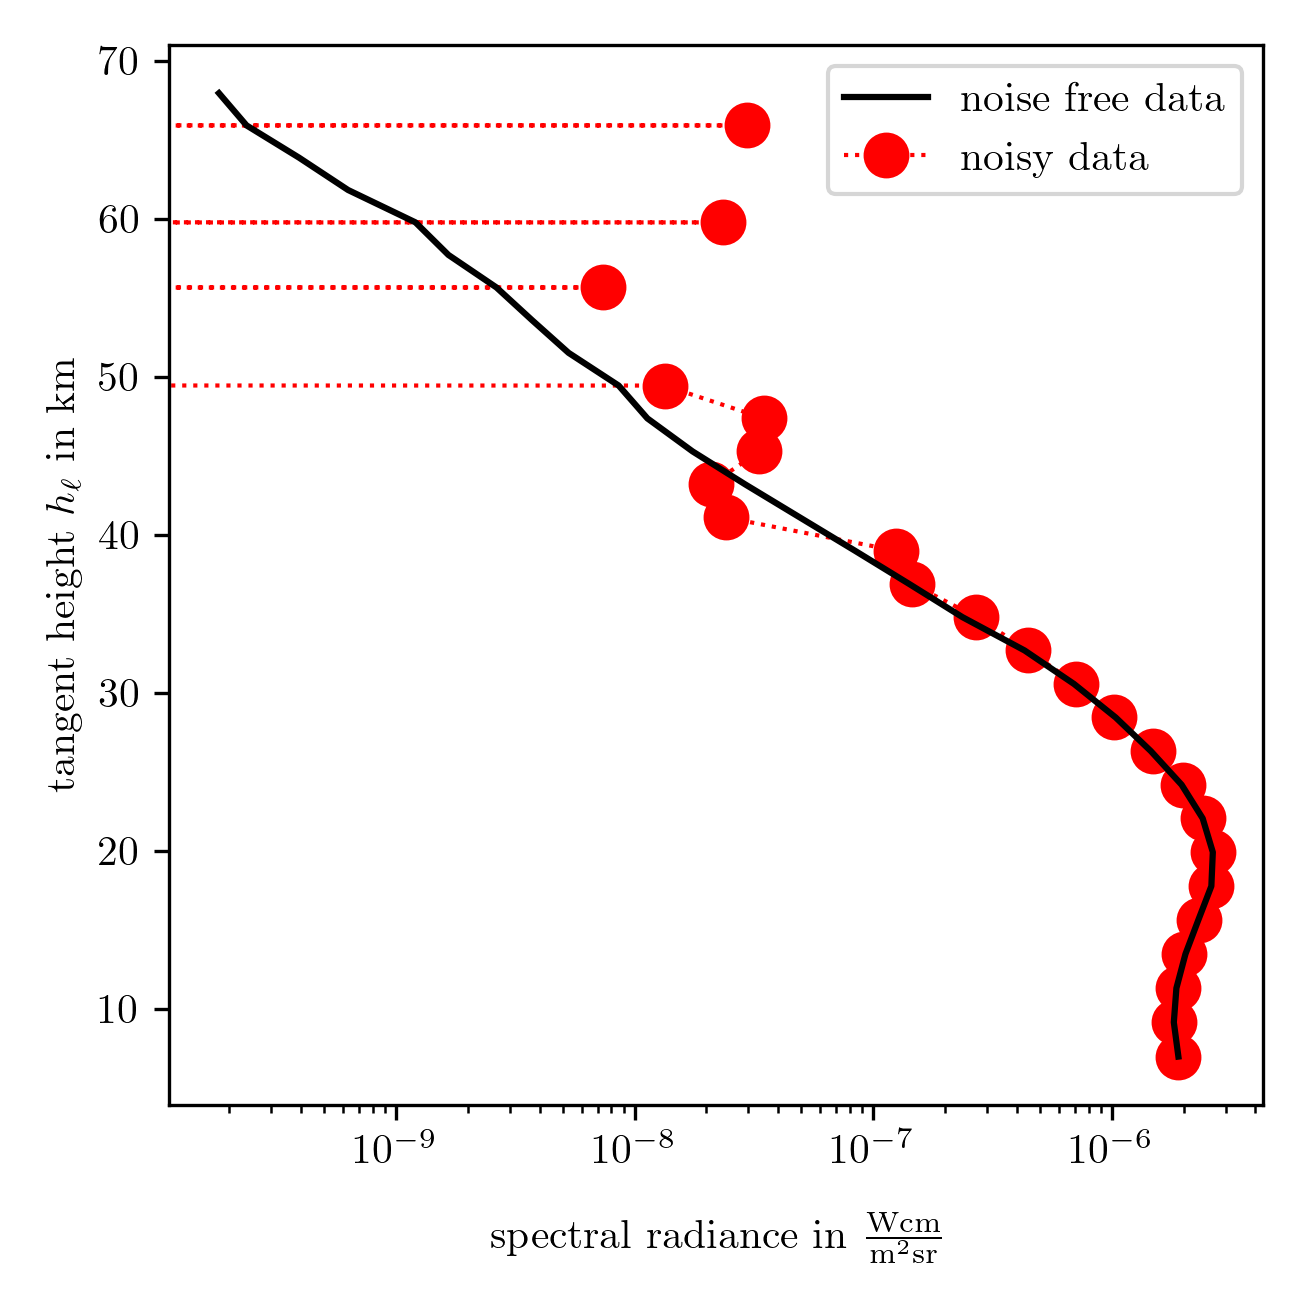
\includegraphics{DataPlot.png}
	\caption[Logarithmic plot of data points at different tangent height.]{Logarithmic plot of data points at different tangent height. Note that negative values are not plotted, and noise is dominating at higher altitudes.}
	\label{fig:DataPlot}
\end{figure}
We plot the data in Fig.~\ref{fig:DataPlot}, which is noise-dominated in higher altitudes and hence not sensitive to structures in the higher atmospheric regions.
Now, given the data, we like to determine the posterior distributions over ozone $\bm{x}$, pressure $\bm{p}$ and temperature $\bm{T}$.
\clearpage


\section{Hierarchical Bayesian Framework for Ozone}
\label{sec:BayModelO3}
\begin{figure}[htb!]
	\centering
	\begin{tikzpicture}
		%box/.style = {draw, thick, minimum width=2.5cm, minimum height=1cm},
		every edge/.style = {draw, -latex, thick} % <---
		\node[roundnode2] at (-4,6.5) (Q)     {$\bm{Q}$};
		\node[roundnode2] at (-2.5,5) (x)     {$\bm{x}$};
		\node[align=center] at (-1,4) (A)    {$\bm{A}$};
		\node[roundnode2] at (-1,2.5) (u)    {$\Omega$};
		\node[rectnode] at (-1,1) (y)    {$\bm{y}$};
		\node[roundnode2] at (-2.5,2.5) (e)    {$\bm{\eta}$};
		\node[roundnode2] at (-6.5,6.5) (S)    {$\bm{\Sigma}$};
		\node[roundnode2] at (-8,8) (s)    {$\gamma$};
		\node[roundnode2] at (-5.5,8) (d)    {$\delta$};
		
		\node[roundnode2] at (-8,10) (shyp)    {$\bm{\theta}_{\gamma}$};
		\node[roundnode2] at (-5.5,10) (dhyp)    {$\bm{\theta}_{\delta}$};
		%Lines
		\draw[->, very thick] (S) -- (e);
		\draw[->, mydotted, very thick] (s) -- (S);
		\draw[->, mydotted, very thick] (e) -- (y);
		\draw[->, very thick] (u.south) -- (y);
		\draw[->, mydotted, very thick] (A) -- (u);
		\draw[->, mydotted,  very thick] (x) -- (A.west);
		\draw[->, very thick] (shyp) -- (s);
		\draw[->, very thick] (dhyp) -- (d);
		
		
		\draw[->, mydotted, very thick] (d) -- (Q); 
		
		\draw[->, very thick] (Q) -- (x); 
		%\node[align=center] at (0,4) (f3) {$= \bm{A}$};
		%\node[align=center] at (0.25,3.95) (f3) {$\approx \bm{M A}_L$};
		\node[align =center] at (-2,8) (T1) {marginal posterior \\ over hyper-parameters \\ $\pi(\delta,\gamma  | \bm{y})$};
		\node[align =center] at (0,5) (T2) {full conditional \\ posterior \\ $\pi( \bm{x} | \delta,\gamma, \bm{y})$ };
		
		%\node[align =center] at (-2.5,10) (T3) {hyper-prior distributions \\ $\pi( \delta, \gamma)$ };
		
		\node[fit=(s)(d),draw,dotted,black, rounded corners] {};
		\draw[->,dotted] (y) edge[bend right=85] (T1);  
		\draw[->,dotted] (T1) -- (T2); 

	\end{tikzpicture} 
	\caption[Directed acyclic graph for ozone retrieval and MTC scheme.]{DAG for visualisation of hierarchical modelling and measuring process of ozone, including the MTC scheme. The hyper-parameter $\gamma$ deterministically (dotted line) sets the noise covariance $\bm{\Sigma} = \gamma^{-1}\bm{I}$ and hence the random (solid line) noise vector $\bm{\eta} \sim \mathcal{N}(0, \gamma^{-1}\bm{I})$.
	The hyper-parameter $\delta$ determines (dotted line) the prior precision matrix $\bm{Q} = \delta \bm{L}$ for the normally distributed (solid line) prior $\bm{x}| \delta \sim \mathcal{N}(0, \delta \bm{L})$, where $\bm{L}$ is a graph Laplacian, see Eq.~\ref{eq:GLapl}.
	The hyper-prior distributions (solid line) $\pi(\delta, \gamma)$ are defined by $\bm{\theta}_{\gamma}$ and $\bm{\theta}_{\delta}$.
	Through a linear forward model $\bm{A}$, we generate a space of all measurable noise-free data $\bm{A}\bm{x}$ from which we randomly observe a data set $\bm{y}$ including some added noise $\bm{\eta}$.
	Within the MTC scheme, we evaluate the marginal posterior over the hyper-parameters $\pi(\gamma, \delta | \bm{y})$ first and then the full conditional posterior $\pi(\bm{x}|\delta,\gamma,\bm{y})$. This breaks the correlation structure of $\bm{x}$ and $\delta$ and $\gamma$, and allows us to evaluate the marginal posterior independent of $\bm{x}$.}
	\label{fig:DAGO3}
\end{figure}
In this section, we set up the hierarchically-ordered linear-Gaussian Bayesian framework to determine the ozone posterior distribution, conditioned on ground truth temperature and pressure.
Where, for now, we define the forward model matrix $\bm{A} \coloneqq \bm{A}_L$ and define the distributions of that Bayesian model, similarly to a regularisation approach, as:
\begin{subequations}
	\begin{align}
		\bm{y} |  \bm{x},\gamma,\delta  &\sim \mathcal{N}(\bm{A} \, \bm{x}, \gamma^{-1} \bm{I}) \label{eq:likelihoodAppl} \\
		\bm{x}| \delta  &\sim \mathcal{N}(\bm{0}, (\delta \bm{L})^{-1} ) \label{eq:priorXAppl} \\
		\delta  &\sim \Gamma(\alpha_{\delta}, \beta_{\delta})\label{eq:priorDelAppl} \\
		\gamma  &\sim \Gamma(\alpha_{\gamma}, \beta_{\gamma})\label{eq:priorGamAppl} \, .
	\end{align} 
	\label{eq:O3BayMode}
\end{subequations}
Assuming Gaussian noise $\bm{\eta} \sim \mathcal{N}(0, \gamma^{-1} \bm{I})$, the likelihood function is a normal distribution with mean $\bm{A} \bm{x}$ and covariance matrix $\gamma^{-1} \bm{I}$.
We define the normal prior-distribution $\pi(\bm{x}|\delta)$ with zero mean and precision matrix $\delta \bm{L}$, where $\delta$ is a smoothness hyper-parameter and $\bm{L}$ is the second order discrete derivate operator (see Eq.~\ref{eq:GLapl}).
Here the hyper-prior distributions $\pi(\delta)$ and $\pi(\gamma)$ are gamma distributions with shape $\alpha$ and rate $\beta$.

We can visualise this hierarchical structure and the correlations between different hyper-parameters and parameters through a DAG, as in Fig.~\ref{fig:DAGO3}.
The hyper-parameter $\gamma$ sets the noise covariance deterministically (dotted line), but is itself statistically (solid line) defined by the hyper-prior distribution $\pi(\gamma)$.
This is a gamma distribution, where $\bm{\theta}_{\gamma}$ determines the shape and rate of $\pi(\gamma)$.
Similarly $\bm{\theta}_{\delta}$ defines $\pi(\delta)$, where $\delta$ accounts for smoothness of the ozone profile and sets the prior precision $\bm{Q}(\delta)$.
Then $\bm{A}\bm{x}$ determines the space of all measurable noise-free data sets $\Omega$ through the linear forward model, from which we observe a data set $\bm{y}$ including some noise $\bm{\eta}$.
Given that data, we ``reverse the arrows'' to determine the posterior distribution $\pi(\bm{x}, \bm{\theta}|\bm{y})$ over the parameter $\bm{x}$ and the hyper-parameters $\bm{\theta}$.
%Since noise is a random process with a defined distribution, the posterior distribution $\pi(\bm{x}|\bm{y})$ is well defined.
Usually, due to underlying correlation structures, evaluating this posterior poses a signifiant challenge.
The MTC scheme breaks this correlation and provides the marginal posterior $\pi(\delta, \gamma | \bm{y})$ first and then the full conditional posterior $\pi(\bm{x}|\delta, \gamma,\bm{y})$.
%Since the forward model described in Ch. \ref{ch:formodel} is weakly non-linear we will set up a linear Bayesian hierarchical framework first based on the linear forward model $\bm{A}_L$ and then later the approximated version $\bm{A}_{NL}\bm{M} \bm{A}_L$.
%Furthermore, the noise is normally distributed, so we establish a linear-Gaussian Bayesian hierarchical framework, aiming to recover an ozone profile and a pressure over temperature profile.
%In doing so, we first draw a directed acyclic graph (DAG) to visualise the measurement and modelling process and determine hyper-parameters and correlations between parameters.
%Then we define prior distributions over all parameters as well as a likelihood function so that we can formulate the posterior distribution.

%In this section, we choose the prior distributions and describe the approach to evaluate the posterior distribution for ozone $\pi(\delta, \gamma, \bm{x}|\bm{y})$, including the noise hyper-parameter $\gamma$.
% we define a linear-Gaussian Bayesian hierarchical model, see Sec. \ref{subsec:LinBay},
%\begin{subequations}
%	\begin{align}
	%		\bm{y} |  \bm{x}, \gamma &\sim \mathcal{N}(\bm{A} \bm{x}, \gamma^{-1} \bm{I}) \label{eq:likelihood} \\
	%		\bm{x} |  \delta &\sim \mathcal{N}(\bm{0}, (\delta \bm{L})^{-1}) \label{eq:xPrior} \\
	%		\delta, \gamma &\sim \pi(\delta, \gamma) \label{eq:gammaPrior},
	%	\end{align}
%	\label{eq:O3BayMode}
%\end{subequations}
%with a normally distributed likelihood $\pi(\bm{y} |  \bm{x}, \gamma)$ including the forward model matrix $\bm{A}$ and prior distributions $\pi(\bm{x} |  \delta)$ and $\pi(\delta, \gamma)$, the noise covariance matrix $\gamma^{-1} \bm{I}$, the prior precision matrix $\delta \bm{L}$ and the prior mean set to zero, as in ~\cite{fox2016fast}.
%The chosen Bayesian model is very similar to the regularisation approach, since we like to show that we receive much more meaningful results compared to a single regularisation solution.

\subsection{Prior Modelling}
\label{subsec:PriorModelO3}
To complete the Bayesian framework, we have to define prior distributions over the hyper-parameters and parameters.
Ideally, we define the prior distributions as uninformative as possible, and include functional dependencies and physical properties.

By choosing a normally distributed prior $\pi(\bm{x}|\delta)$ with zero mean and no other restrictions, it is clear that our model does not take into account that ozone values cannot be negative.
As already mentioned, we set the precision matrix of that prior distribution to
\begin{align}
	\delta \bm{L} =
	\delta
	\begin{bmatrix}
		2 & -1 & & &  \\
		-1 & 2 & -1 & &   \\
		& \ddots & \ddots & \ddots &\\ 
		& & -1 & 2 & -1  \\
		& & & -1 & 2 
	\end{bmatrix} 
	\label{eq:GLapl} 
\end{align}
which is a 1-dimensional Graph Laplacian as in~\cite{wang2015graphs,fox2016fast} with Dirichlet boundary condition.
This matrix will also act as the regulariser later in Sec.~\ref{sec:regularise}.
We reduce the dimension of $\bm{x}$ from $45$ to $34$ by discarding every second ozone VMR over a height of $\approx47$km.
Doing that, while not changing $\bm{L}$, we effectively induce a larger correlation between points at higher altitude.
We plot the corresponding prior ozone profiles according to $\bm{x}\sim \mathcal{N}(0, (\delta \bm{L})^{-1})$ in Fig.~\ref{fig:O3Prior}.

For $\delta$ and $\gamma$ we pick relatively uninformative gamma distributions so that $\gamma \sim \mathcal{T}(\bm{\theta_{\gamma}}) \propto \gamma^{\alpha_\gamma -1 } \exp{( -\beta_\gamma \gamma) } $ and $\delta \sim \mathcal{T}(\bm{\theta_{\delta}})$, where $\bm{\theta_{\gamma}} = \{  \alpha_\gamma, \beta_\gamma\}  = \{ \alpha_\delta ,\beta_\delta\} = \bm{\theta_{\delta}} = (1,10^{-35})$ (see Fig.~\ref{fig:MargPostHistTT}) similar to \cite{fox2016fast}.
Those gamma distributions have another advantage when using the MWG algorithm to sample from the marginal posterior distribution $\pi(\delta, \gamma | \bm{y})$, where then $\pi(\gamma | \lambda, \bm{y}) \sim \mathcal{T}(\cdot)$ is a gamma distribution with $\lambda = \delta / \gamma $, and easy to sample from.

\subsection{Posterior Distribution -- Linear Model}
\label{sec:FirstO3Post}
As explained in Sec.~\ref{subsec:TheoMTC},we factorise the posterior
\begin{align}
	\pi( \bm{x}, \delta, \gamma| \bm{y}) \propto \pi(\bm{y}| \bm{x},\delta,\gamma) \pi( \bm{x},  \delta,\gamma)
\end{align}
into 
\begin{align}
	\pi( \bm{x},  \delta,\gamma| \bm{y}) =\pi( \bm{x}| \delta,\gamma, \bm{y})\pi( \delta,\gamma | \bm{y})
\end{align}
the marginal posterior $\pi(\delta ,\gamma| \bm{y})$ and full conditional posterior $\pi( \bm{x}| \delta,\gamma, \bm{y})$ (see Eq.~\ref{eq:MTC}).
%Fox and Norton call this method the marginal and then conditional method (MTC) \cite{fox2016fast}, where we break the correlation structure between $\bm{x}$ and $\gamma, \delta$ as illustrated in Fig. \ref{fig:RueHeld} by marginalising over $\bm{x}$.
As discussed in Sec.~\ref{subsec:LinBay}, for the linear-Gaussian case, $\bm{x}$ cancels in the marginal posterior over the hyper-parameters.
Following the MTC scheme, we characterise the marginal posterior first and then the full conditional posterior.

\subsubsection{Marginal posterior}
\label{subsec:FirstMargPost}
Consequently, for the hierarchical model specified in Eq.~\ref{eq:O3BayMode}, the marginal posterior distribution over the hyper-parameters is given by
\begin{align}
	\pi( \lambda,\gamma  | \bm{y}) \propto &  \lambda^{n/2 + \alpha_{\delta}-1} \gamma^{m/2 + \alpha_{\delta} + \alpha_{\gamma}-1}   \exp{ \Bigl\{ - \frac{1}{2} g ( \lambda) - \frac{\gamma}{2} f ( \lambda) - \beta_{\delta} \lambda  \gamma - \beta_{\gamma} \gamma \Bigr\}},
	\label{eq:MargPostAppl}
\end{align}
with the introduced regularisation parameter $\lambda = \delta / \gamma$, and
\begin{subequations}
	\begin{align}
		&f ( \lambda) = \bm{y}^T \bm{y} - (\bm{A}^T \bm{y})^T (\bm{A}^T  \bm{A} + \lambda \bm{L})^{-1} (\bm{A}^T \bm{y})  \label{eq:fAppl} \, ,  \\
		&\text{and } g(\lambda) = \log \det (\bm{A}^T  \bm{A} + \lambda \bm{L}) \label{eq:gAppl} \, .
	\end{align}
\end{subequations}
Note that when changing variables from $\delta = \lambda \gamma$ to $\lambda$ the hyper-prior distribution changes to $\pi(\lambda) \propto \lambda^{\alpha_{\delta}-1} \gamma^{\alpha_{\delta}} \exp{(- \beta_{\delta} \lambda  \gamma)} $, due to $\text{d}\delta / \text{d} \lambda = \gamma$.
\begin{figure}[th!]
	\centering
	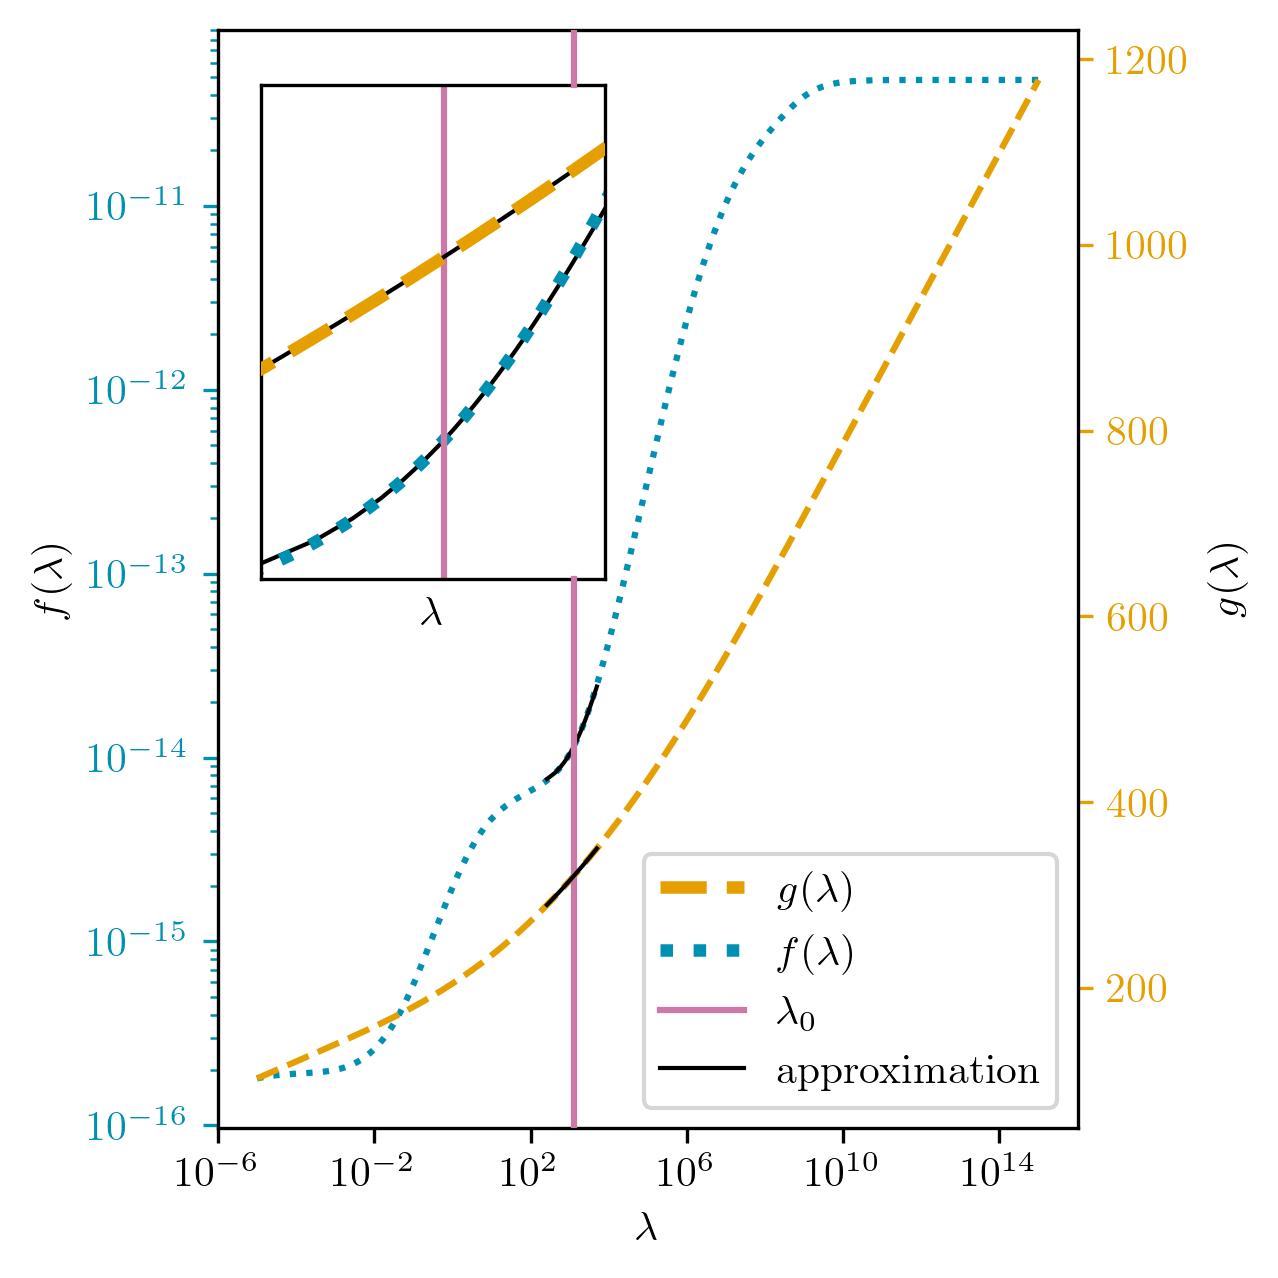
\includegraphics{f_and_g_phd.png}
	\caption[Functions $f(\lambda)$ and $g(\lambda)$ of 2D marginal posterior.]{Functions $f(\lambda)$ and $g(\lambda)$ from the marginal posterior in Eq.~\ref{eq:MargPostAppl} for a wide range of $\lambda = \delta / \gamma$. We plot the approximations (see Eq.~\ref{eq:fAprox} and Eq.~\ref{eq:gAprox}) in black around the mode of the marginal posterior (vertical line) for the sampling range of $\lambda$ within the MWG algorithm.}
	\label{fig:fandg}
\end{figure}
For each evaluation of the marginal posterior most of the computational effort lies in the calculation of $f(\lambda)$ and $g(\lambda)$, which we evaluate using the Cholesky decomposition $\bm{A}^T  \bm{A} + \lambda \bm{L} = \bm{C}_{\lambda} \bm{C}_{\lambda}^T$.
More specifically we solve for $(\bm{A}^T  \bm{A} + \lambda \bm{L})^{-1} (\bm{A}^T \bm{y})$ via \texttt{scipy.linalg.cho\_solve} and calculate the $g(\lambda) = 2 \sum \log \text{diag}(\bm{C}_{\lambda}) $.
In  Fig.~\ref{fig:fandg} we see that $f(\lambda)$ and $g(\lambda)$ are well behaved within the region of interest.
Because of this, we approximate $f(\lambda) \approx \tilde{f}(\lambda)$ with a Taylor series and $\tilde{g}(\lambda) \approx g(\lambda)$ with a linear approximation in log-space around the mode $\lambda_0$ of $\pi(\lambda, \gamma | \bm{y})$.
The approximations are implicitly given by
\begin{align}
	f^{(r)}& (\lambda_0)= (-1)^{r+1} (\bm{A}^T \bm{y})^T (\bm{B}_0^{-1} \bm{L})^r \bm{B}_0^{-1} \bm{A}_L^T \bm{y} \label{eq:ftay}  \\
	\text{and } & \log{ \tilde{g}(\lambda)} = \log{ g(\lambda_{0})} + (\log{\lambda} - \log{\lambda_{0}})  \frac{ \log{g(\lambda_{\text{max}})} - \log{g(\lambda_{0})} }{\log{\lambda_{\text{max}}} - \log{\lambda_{0}} } 
	\label{eq:gtay}
\end{align} 
with $\bm{B}_0 = \bm{A}^T  \bm{A} + \lambda_0 \bm{L}$.
We plot the approximations
\begin{subequations}
	\label{eq:fandgapprox}
	\begin{align}
		&\tilde{f} ( \lambda) = \sum^2_{r=0} 	f^{(r)}(\lambda_0) (\lambda-\lambda_0)^r  \label{eq:fAprox} \, ,  \\
		&\text{and } \tilde{g} (\lambda) = \exp \log{\tilde{g}(\lambda)}  \label{eq:gAprox} \, ,
	\end{align}
\end{subequations} in Fig.~\ref{fig:fandg} and elaborate on the approximation errors in the section below.
Usually a Taylor series includes a factor $(r!)^{-1}$, which in this case cancels in $f^{(r)}(\lambda_0)$, and $g(\lambda)$ can be approximated with a Taylor series as well (see~\cite{fox2016fast}).

\paragraph{Error due to approximation of f and g}
To assess the approximation error, we lay a 100-point grid over the sampling region in each dimension and compare the approximations of $f(\lambda)$, $g(\lambda)$ and $\pi(\lambda, \gamma | \bm{y})$ with their true function values.

\textcolor{red}{Compared to a 1-st, 3-rd or 4-th order Taylor approximation, we find that the 2-nd order Taylor approximation of $f(\lambda)$ gives the smallest relative RMS error of $\approx 10 \%$ in the sampling region of $\lambda$.
Additionally, we find that a linear approximation of $g(\lambda)$ is sufficient with relative RMS $<0.1\%$.}

These errors then propagate into the marginal posterior $\pi(\lambda , \gamma| \bm{y})$ so that the relative RMS error is $\approx 3 \%$ over the whole grid.
When sampling, we evaluate the acceptance ratio in the log-space, so we report a relative RMS error of $< 0.01\%$ for $\log{\pi(\lambda| \gamma, \bm{y})}$, with a maximum relative pointwise error of $< 0.5\%$.
We consider this good enough.

\paragraph{Sample from marginal posterior}
Using these approximations, we employ a Metropolis within Gibbs (MWG) sampler (see Alg. Box \ref{alg:MwG}) to characterise $\pi(\lambda,\gamma|\bm{y})$ (see Sec.~\ref{subsec:MWG}).

We approximate $f(\lambda)$  and $g(\lambda)$ around the mode $( \lambda_{0}, \gamma_0 )$ of $\pi(\lambda,\gamma| \bm{y})$ provided by the \texttt{scipy.optimize.fmin} function, with a limit of 25 function evaluations.
Then we approximate $f(\lambda)$ with a 2-nd order Taylor series and $g(\lambda)$ with a linear approximation in the log-space, where for the approximation in $g(\lambda)$ we set $\lambda_{\text{max}}$ to the maximum value of $\lambda$ on the TT grid (see next section).

We initialised the MWG algorithm at the mode $(\lambda^{(0)} , \gamma^{(0)}  ) = ( \lambda_{0} , \gamma_{0}  )$ and take $N = 10000$ plus $N_{\text{burn-in}} = 100$ steps in $\approx 0.5$s.
The standard deviation of the normal proposal distribution is empirically set to $\sigma_{\lambda} = 0.8 \lambda_0$, so that the acceptance rate is $\approx 0.5$ as suggested in~\cite{robertsLecNot}.
More specifically, we implement a Metropolis random walk on
\begin{align}
	\label{eq:margApplCondGam}
	\pi(\lambda | \gamma, \bm{y}) &\propto \lambda^{n/2 +\alpha_{\delta}-1} \exp{\Bigl\{ - \frac{1}{2} g ( \lambda) - \frac{\gamma}{2} f ( \lambda) - \beta_\delta \gamma \lambda \Bigr\}}.
\end{align} 
In doing so, we accept $\lambda^{k+1} = \lambda^{\prime} $ or reject $\lambda^{k+1} = \lambda^{k}$ a proposal $\lambda^{\prime} \sim \mathcal{N}(0, \sigma^2_{\lambda})$ according to the acceptance ratio
\begin{align}
	\alpha(\lambda^{\prime} |  \lambda^{k} ) = \min \left\{ 1, \frac{\pi(\lambda^{\prime} | \gamma^{(k)}, \bm{y})  }{\pi(\lambda^{(k)}| \gamma^{(k)}, \bm{y})} \right\} \, .
\end{align}
In practice, we calculate the acceptance ratio in log space, so that
\begin{align} 
	\log \left\{ \frac{\pi(\lambda^{\prime} | \gamma^{(k)}, \bm{y})  }{\pi(\lambda^{(k)}| \gamma^{(k)}, \bm{y})}  \right\} 
	= \log  \{\pi(\lambda^{\prime} | \gamma^{(k)}, \bm{y} ) \}  -\log  \{ \pi(\lambda^{(k)}| \gamma^{(k)}, \bm{y}) \} \\
	= \frac{n}{2} (\log\{\lambda^{\prime}\} - \log\{\lambda^{(k)}\} ) + \frac{1}{2} \Delta g + \frac{\gamma^{(k)}}{2} \Delta f  + \beta_\delta \gamma^{(k)} \Delta \lambda  \, ,
\end{align}
where $\Delta \lambda = \lambda^{\prime} - \lambda^{(k)} $ and  $\Delta f \approx \tilde{f}(\lambda^\prime) - \tilde{f}(\lambda^{(k)}) =  \sum^2_1 f^{(r)} (\lambda_0) [(\Delta \lambda^\prime)^r - (\Delta \lambda^{(k)})^r] $, with  $\Delta \lambda^{\prime} = \lambda^\prime - \lambda_0 $ and $\Delta \lambda^{(k)} =  \lambda^{(k)} - \lambda_0$.
Similarly we approximate $\Delta g \approx \tilde{g}(\lambda^{\prime}) -\tilde{g}(\lambda^{(k)})$.
Lastly, we do a Gibbs step on
\begin{align}
	\gamma^{(k+1)} |  \lambda^{(k+1)}, \bm{y} &\sim \Gamma \bigg( \frac{m}{2} + \alpha_\delta + \alpha_\gamma, \frac{1}{2} f (\lambda^{(k+1)}) + \beta_\gamma + \beta_\delta \lambda^{(k+1)} \bigg)\label{eq:GibbsStep}
\end{align} 
to generate marginal posterior samples $(\lambda, \gamma)^{(1)}, \dots, (\lambda, \gamma)^{(N)} \sim  \pi(\lambda, \gamma| \bm{y})$, which we plot in Fig.~\ref{fig:ScatterPlotTT} as well as the trace of the MWG to show ergodicity.
%
%We find the mode at the minimum of  $-\log\{ \pi(\lambda, \gamma | \bm{y}) \}$  using \texttt{scipy.optimize.fmin} function and limit the number of function evaluation to 25 and use Cholesky back and forward substitution to calculate values of $g(\lambda)$ and $f(\lambda)$.
%Additionally, we calculate $\bm{B}_0^{-1} \bm{L} $ and  $\bm{B}_0^{-1}  \bm{A}_L^T \bm{y}$ once more at $\lambda_0$ and plot the Taylor approximation within the sampling region in Fig. \ref{fig:fandg}.
%\subsection{Posterior distributions with Linear model for Ozone -- MTC}
%\label{sec:firstMTC}
%In this section we calculate the posterior marginal and then conditional (MTC) posterior distribution for ozone conditioned on the ground truth temperature and pressure profiles using the linear forward model $\bm{A}_L$.
%This is faster then the other way round (finding temperature over pressure conditioning on ozone) and temperature and pressure are well defined within the atmosphere so it is easier to just condition on a temperature and pressure profile out of a text book.
%We employ a so-called Metropolis within Gibbs (MWG) algorithm on the marginal posterior as summarised in the algorithmic Box \ref{alg:margPost} or use a Tensor-Train (TT) approximation to calculate marginal posterior values.
%Then we can either sample from the conditional posterior using the randomise then optimise (RTO) method or calculate conditional mean and variance using quadrature.
%The DAG in Fig. \ref{fig:DAGO3} visualises that process and we can show explicitly that we group the hyper-parameters $\delta, \gamma$ together to determine the marginal posterior $\pi(\gamma, \delta | \bm{y})$.
%Here $\gamma$ , the noise parameter, determines the noise precision $\bm{\Sigma} = \gamma ^{-1} \bm{I}$ and $\delta$, the smoothness parameter, the precision matrix $\bm{Q} = \delta \bm{L}$ of the prior distribution for $\bm{x}$.
%Then conditioned on the hyper-parameters the conditional posterior $\pi( \bm{x} |\gamma, \delta, \bm{y})$ gives the distribution of posterior ozone profiles.
%Note that we use the linear model $A_L$ here as we do not have an approximation to the non-linear model yet and all prior distributions are defined in Table \ref{tab:priors}.
%The full posterior $\pi(\bm{x},\gamma, \delta | \bm{y}) =  \pi(\bm{x}|\gamma, \delta ,\bm{y}) \pi(\gamma, \delta | \bm{y}) $ is given by multiplication of the marginal and conditional posterior densities. 
%\begin{align}
%	\bm{x} |  \bm{\theta}, \bm{y} \sim \mathcal{N} \Big(
%	\underbrace{\bm{\mu} + \left( \bm{A}^T \bm{\Sigma}^{-1} \bm{A} + \bm{Q} \right)^{-1} \bm{A}^T \bm{\Sigma}^{-1} (\bm{y} - \bm{A} \bm{\mu})}_{\bm{\mu}_{\bm{x} |  \bm{\theta}, \bm{y}}},
%	\underbrace{ \left( \bm{A}^T \bm{\Sigma}^{-1} \bm{A} + \bm{Q} \right)^{-1} }_{\bm{\Sigma}_{\bm{x} |  \bm{y}, \bm{\theta}}}
%	\Big) \, ,
%\end{align}
%is normal distribution and we compute weighted expectations, as in Eq.~\ref{eq:MargExpPos}, of the conditional mean and covariance matrix, where the weights are given by $\pi(\bm{\theta} | \bm{y})$. 
%Note that both the noise covariance $\bm{\Sigma} = \bm{\Sigma}(\bm{\theta})$ and the prior precision matrix $\bm{Q} = \bm{Q}(\bm{\theta})$ depend on the hyper-parameters $\bm{\theta}$.
We calculate the IACT with the Python implementation of~\cite{wolff2004monte} provided by~\cite{drikHesse}, which gives us $\tau_{\text{int}, \gamma} \approx 4.4 \pm 0.2$ and $\tau_{\text{int}, \lambda} = 10.4 \pm 1.0 $ (see Fig.~\ref{fig:IATCLamLin} and Fig.~\ref{fig:IATCGamLin}).
\begin{figure}[h!]
	\centering
	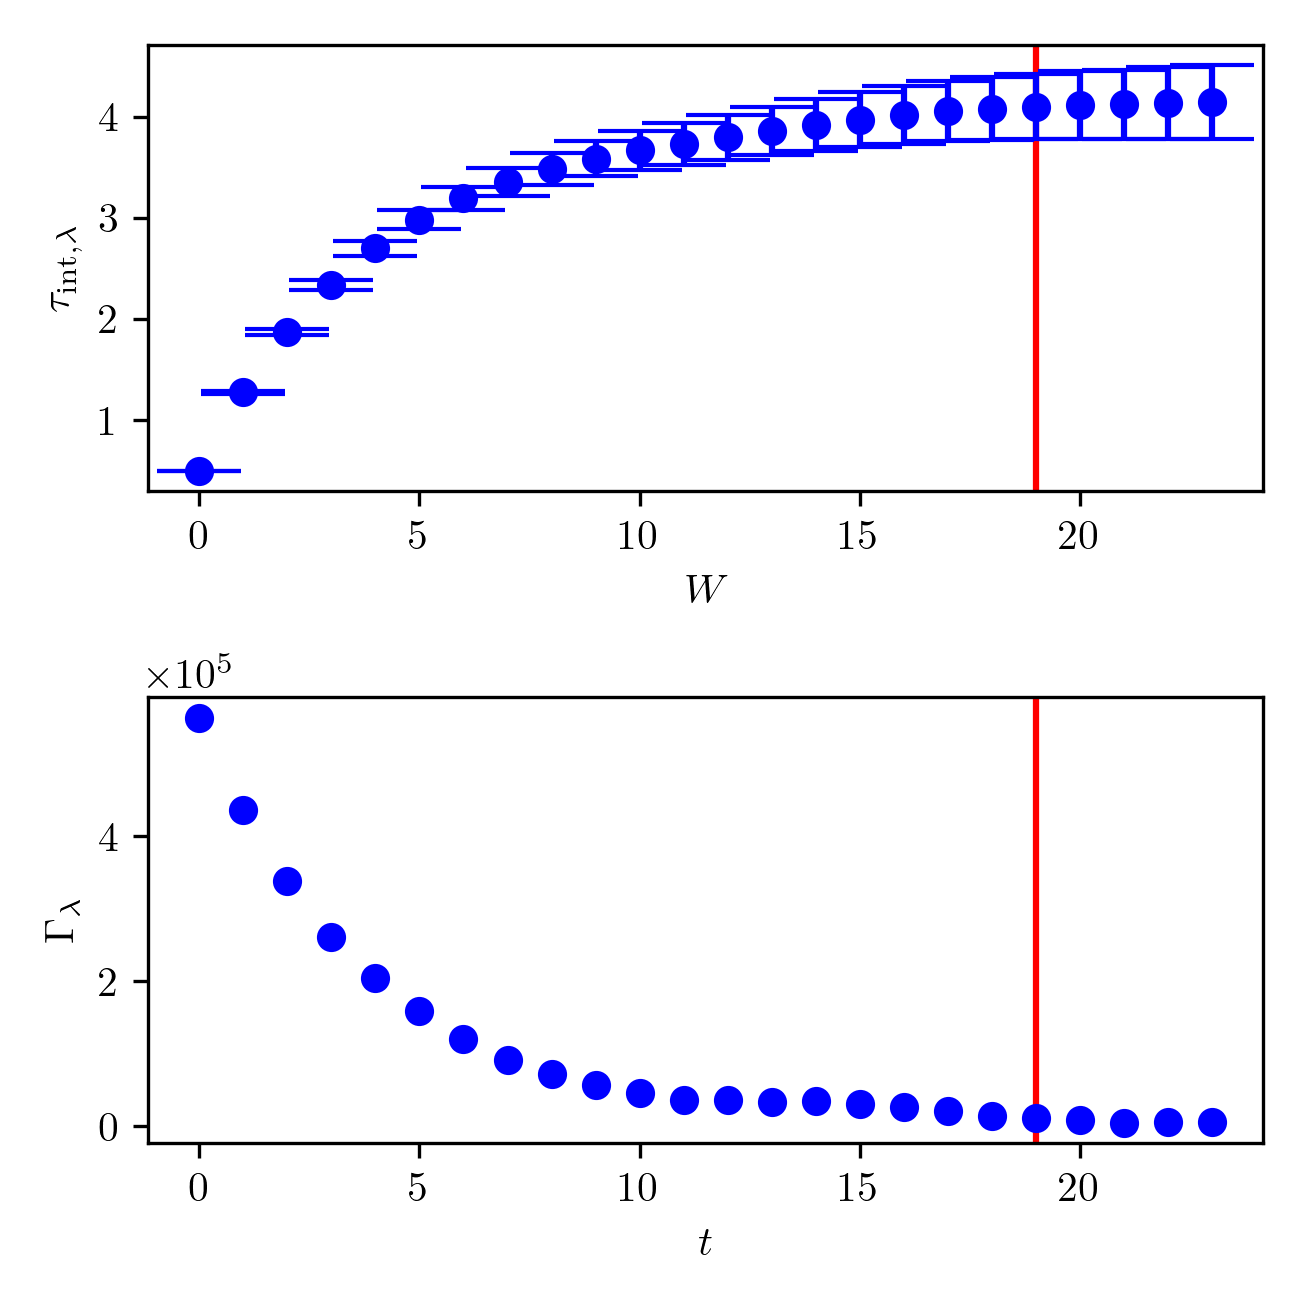
\includegraphics{UwerrTauIntFirstO3lam.png}
	\caption[IACT of $\lambda \sim \pi( \cdot| \bm{y})$, for linear model.]{Provided by \cite{drikHesse}, the IACT $\tau_{\text{int},\lambda}$ at summation windows W as well as the estimated autocorrelation function $\Gamma_{\lambda}$ at lag $t$ of the samples $\lambda \sim \pi( \cdot| \bm{y})$.}
	\label{fig:IATCLamLin}
\end{figure}


\paragraph{TT approximation of marginal posterior}
Alternatively, we can utilise a TT approximation of the square root of the marginal posterior over a predefined grid and calculate the marginals $\pi(\gamma|\bm{y})$ and $\pi(\lambda|\bm{y})$ (see Sec. \ref{subsec:TTMarg}).

\textcolor{red}{We predefined the univariate grid with $n = 20$ grid points (see Fig. \ref{fig:MeanVarError}) over $\gamma = [ 0.25 \times 10^{15}, 6 \times 10^{15}]$ and $\lambda = [ 1, 5000]$.}
We introduce a ``normalisation constant'' $c = - 340/2$ to avoid underflow so that the values of $\sqrt{\pi( \lambda,\gamma| \bm{y})} = \exp \{ 0.5 \log  \pi(\lambda,\gamma | \bm{y}) + c \} $ are within computer precision.
Then we initialise the~\texttt{tt.cross.rectcross.rect\_cross.cross} function based on the TT cross algorithm in \cite{OSELEDETS2010TTCross,Dolgov2018TTCross} from the Python package \texttt{ttpy}~\cite{Oseledets2018ttpy} with a random tensor.
The number of ranks is set to constant $r = 4$, we do 1 sweep with $2n_{\text{sweeps}}2nr =400$ function evaluations and obtain a TT approximation of $\pi( \lambda,\gamma| \bm{y})$ in about $0.02$s.
Ironically, this the same number of functions evaluations to approximate a $20 \times 20$ point grid.
The TT format is especially advantageous for larger grid sizes and higher dimensional parameter spaces.
To compute the marginals $\pi(\lambda| \bm{y})$ and $\pi(\gamma| \bm{y})$ we set the TT error $\xi = 1 / \uplambda (\mathcal{X})$ and $\uplambda(x) = 1$, so that for Cartesian basis $\bm{M}_k = \text{diag}(\uplambda_k(\mathcal{X}_k))$ (see Eq.~\ref{eq:MassMat}).
We calculate the coefficient tensor $\bm{B}$ and $\bm{R}_{\text{pre}}$ as in Prop.~\ref{prob:backMarg} and Prop.~\ref{prob:ForMarg} (see Sec.~\ref{subsec:TTMarg}).

We plot the TT approximation as a colour map on top of the obtained samples in Fig.~\ref{fig:ScatterPlotTT}.
The relative RMS TT approximation error over the whole grid is $\approx 3\%$ and similar to the propagation error in $\pi(\lambda, \gamma| \bm{y})$ due to the approximations of $f(\lambda)$ and $g(\lambda)$ (see further up).
\begin{figure}[h!]
	\centering
	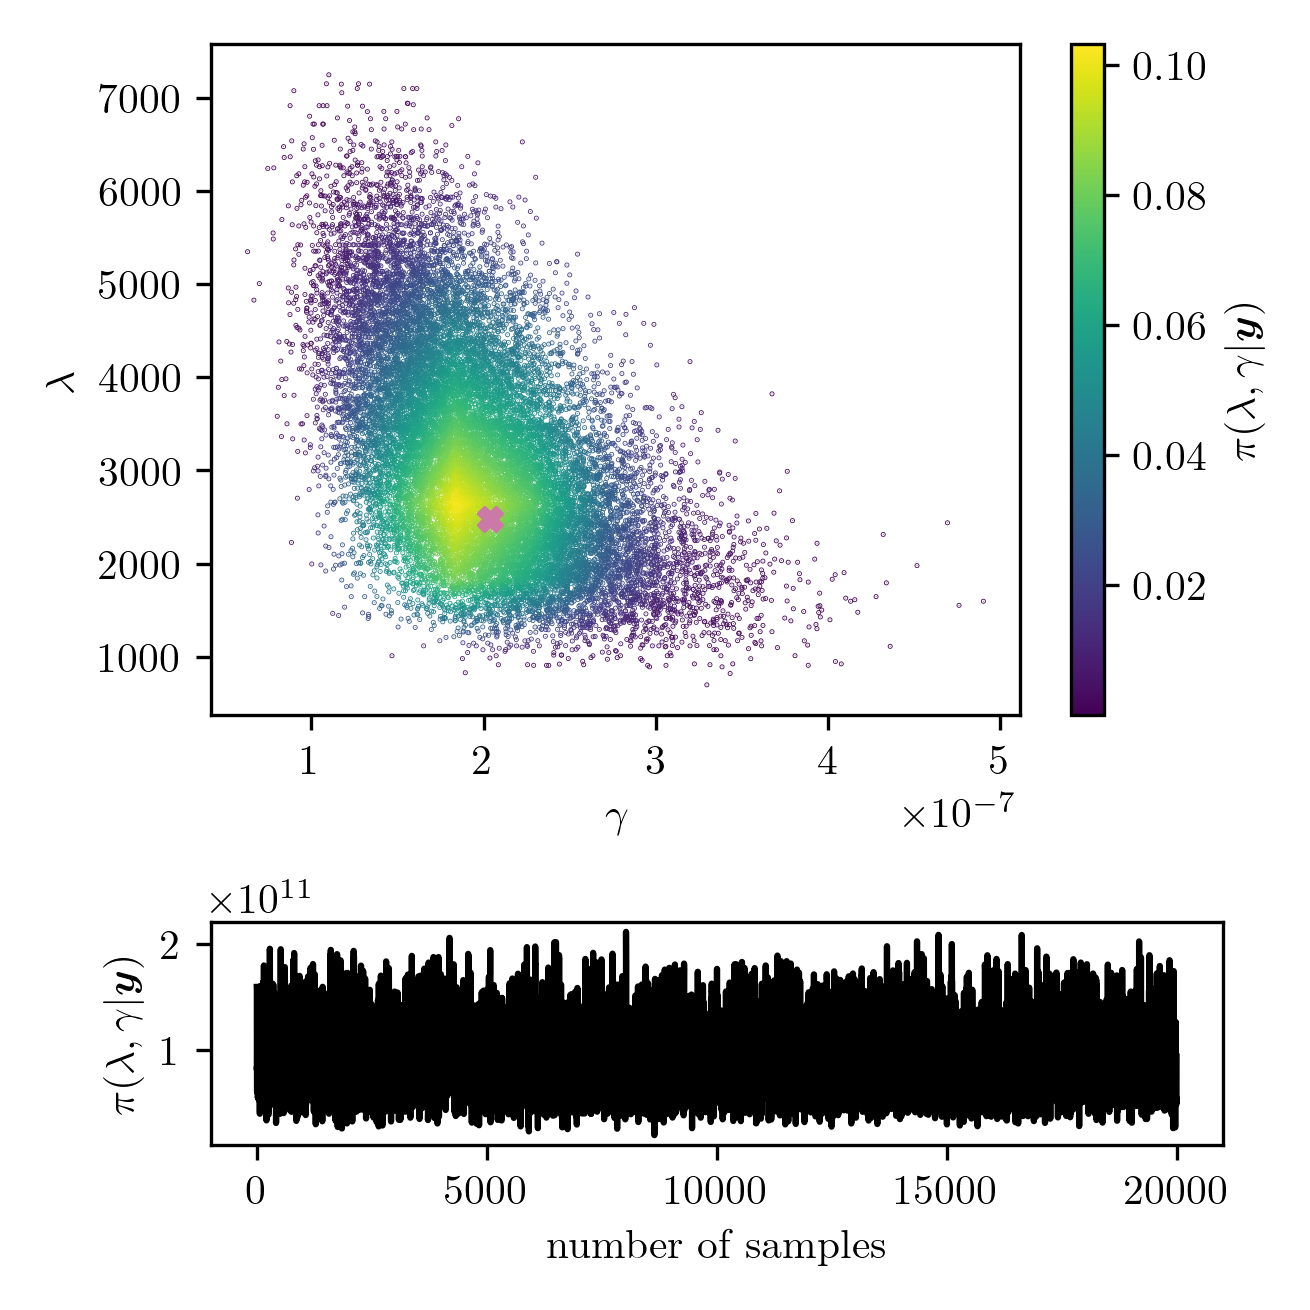
\includegraphics{ScatterplusHistoPlusTT.png}
	\caption[Samples from marginal posterior and TT approximation; trace plot of the MWG for $\pi(\lambda, \gamma| \bm{y})$]{Samples from the marginal posterior colour-coded using the TT approximation of $\pi(\lambda , \gamma  | \bm{y})$. The mode of $(\lambda_0 , \gamma_0)$ of $\pi(\lambda , \gamma  | \bm{y})$ is marked with the pink cross. To show ergodicity, we plot the trace of the samples of the MWG algorithm.}
	\label{fig:ScatterPlotTT}
\end{figure}
%\subsubsection{Sample from Marginal Posterior Distribution}
%\label{subsec:firstMarg}

%\begin{algorithm}[!ht]
%	\caption{Metropolis within Gibbs for $\pi(\lambda, \gamma | \bm{y})$}
%	\begin{algorithmic}[1]
%		\STATE Initialise  \( \bm{\theta}^{(0)}  =( \lambda^{(0)} , \gamma^{(0)}  ) \) and set burn-in $N_{\text{burn-in}}$
%		\FOR{ \( k = 1, \dots, N^{\prime} \)}
%		\STATE Propose \( \lambda \sim \mathcal{N}(\lambda^{(t-1)}, 0.8 \lambda_0)  \)
%		\STATE Compute
%		\[ \alpha( \lambda  | \lambda^{(t-1)}) = \min \left\{ 1, \frac{\pi(\lambda | \gamma^{(t-1)}, \bm{y})  }{\pi(\lambda^{(t-1)}| \gamma^{(t-1)}, \bm{y})}  \right\} \]
%		\STATE Draw $u \sim \mathcal{U}(0,1)$
%		\IF{$\alpha \geq u$ }
%		\STATE Accept and set \( \lambda^{(t)} = \lambda \)
%		\ELSE  
%		\STATE Reject and keep \(\lambda^{(t)} = \lambda^{(t-1)} \)
%		\ENDIF
%		\STATE Draw $\gamma^{(t)} | \lambda^{(t)} ,\bm{y} \sim \text{Gamma} \big( 0.5  \, m + 2, 0.5 \, f(\lambda^{(t)}) + 10^{-10}(1 + \lambda^{(t)}) \big) $
%		\ENDFOR
%		%\STATE Output: $ \bm{\theta}^{(N_{\text{burn-in}})}, \dots,  \bm{\theta}^{(k)} , \dots,   \bm{\theta}^{(N)} \sim \pi(\bm{\theta}| \bm{y}) $
%		\STATE Output: $ (\lambda, \gamma)^{(N_{\text{burn-in}})}, \dots,  (\lambda, \gamma)^{(k)} , \dots,   (\lambda, \gamma)^{(N)} \sim \pi(\lambda, \gamma| \bm{y}) $
%	\end{algorithmic}
%	\label{alg:margPost}
%\end{algorithm}
\subsubsection{Full posterior ozone mean and variance}
\label{subsec:firstCond}
\begin{figure}[ht!]
	\centering
	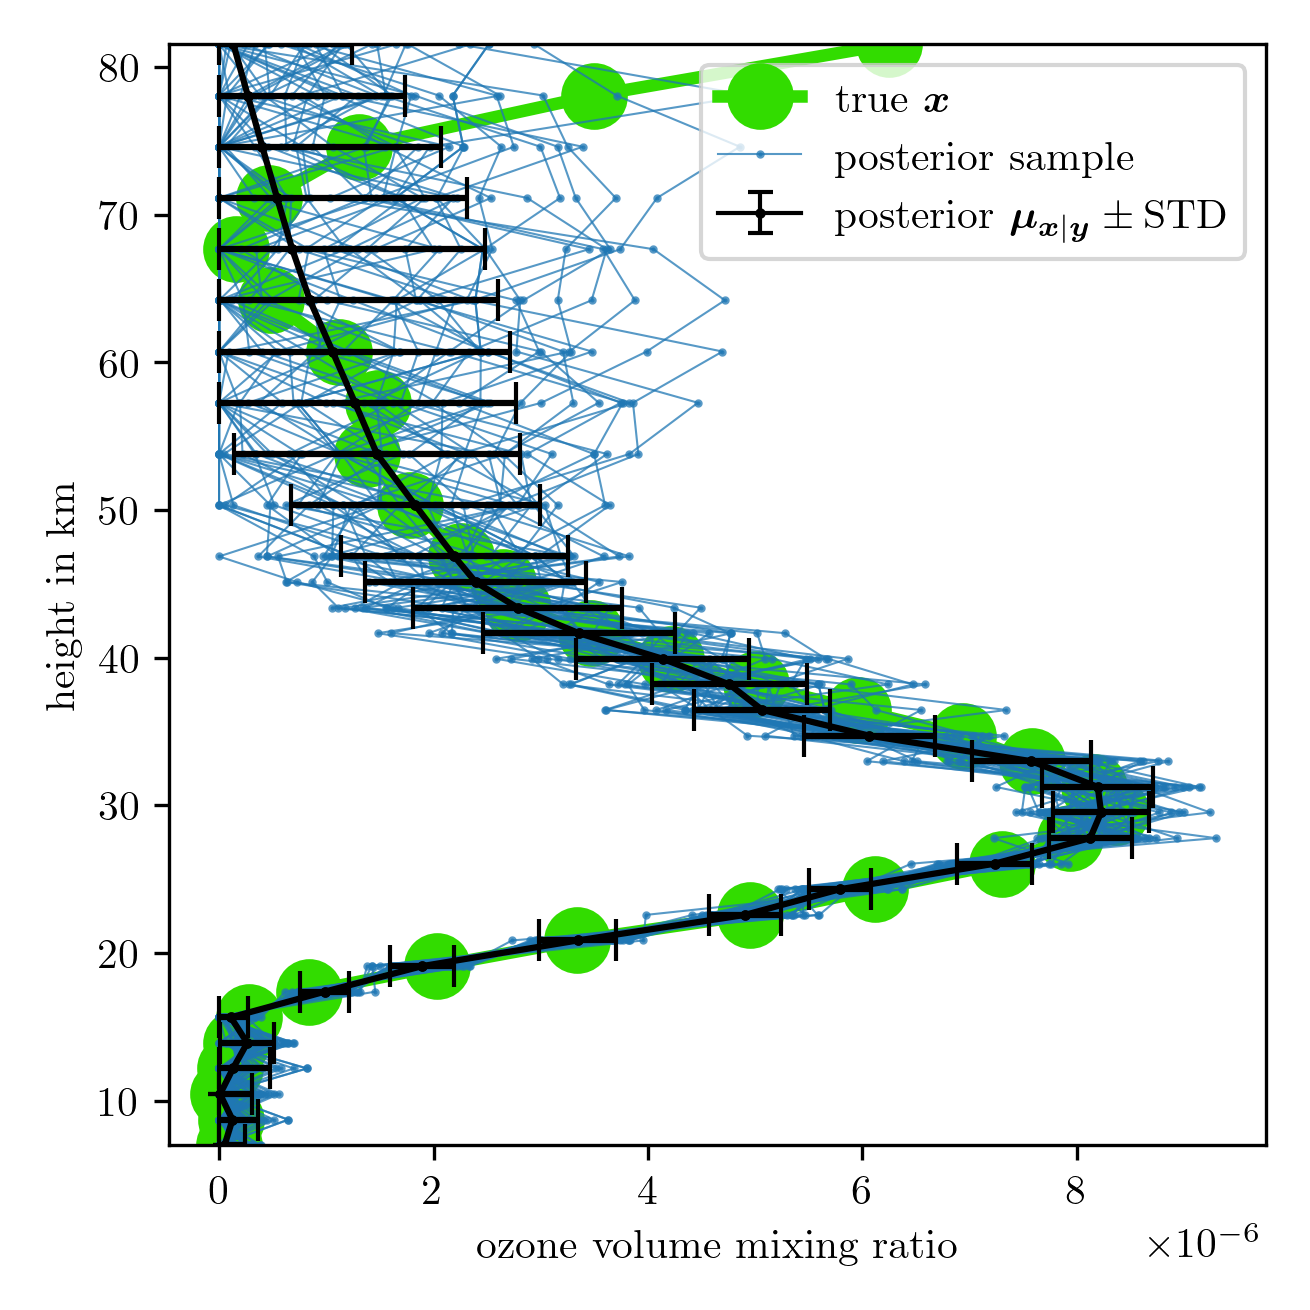
\includegraphics{FirstTestRes.png}
	\caption[Ozone samples of the full posterior.]{Ozone samples from the full posterior distribution $\pi(\bm{x}| \bm{y})$ after characterising full posterior mean and covariance by weighted expectations over the marginal posterior $\pi(\lambda,\gamma | \bm{y})$ based on the linear forward map $\bm{A}_L$. We set negative ozone VMR values to zero.}
	\label{fig:O3Samp}
\end{figure}
Finally, we evaluate the normally distributed full conditional posterior distribution
\begin{align}
	\bm{x}| \delta, \gamma, \bm{y}  \sim \mathcal{N}\big( \underbrace{ (\bm{A}^T \bm{A} + \delta / \gamma \bm{L} )^{-1} \bm{A}^T \bm{y}}_{\bm{x}_{\lambda}}, ( \underbrace{ \gamma \bm{A}^T \bm{A} + \delta \bm{L} }_{\gamma \bm{B}_{\lambda}}  )^{-1} \big) \, \label{eq:CondPost},
\end{align}
as in Eq. \ref{eq:CondPostLin}, with $\lambda = \delta / \gamma $.
In this thesis, we compute the mean
\begin{align}
	\mu_{\bm{x}|\bm{y}} = \int \bm{x}_{\lambda} \pi(\lambda| \bm{y}) \diff\lambda \approx \sum \bm{x}_{\lambda_i} \pi(\lambda_i| \bm{y}) \, , \label{eq:MeanInt}
\end{align} and covariance
\begin{align}
	\Sigma_{\bm{x}|\bm{y}} = \int \gamma^{-1}  \pi(\gamma | \bm{y} ) \, \diff \gamma \, \int  \bm{B}_{\lambda}^{-1} \, \pi(\lambda | \bm{y} )  \, \text{d} \lambda  \approx \sum {\gamma_i}^{-1}\pi(\gamma_i| \bm{y}) \sum \bm{B}_{\lambda_i}^{-1}\pi(\lambda_i| \bm{y})\, \label{eq:CovInt}
\end{align}
of $\pi(\bm{x}| \bm{y})$ as weighted expectations over the marginal posterior $\pi(\lambda,\gamma | \bm{y})$ by quadrature \cite[Sec. 2.1]{Dick_Kuo_Sloan_2013} with $\sum \pi(\lambda_i| \bm{y}) = \sum \pi(\gamma_i| \bm{y}) = 1$.
The weights $\pi(\lambda_i| \bm{y})$ and $\pi(\gamma_i| \bm{y})$ are either given by the TT approximation or by the bars of the sample-based histograms.
More precisely, the heights of the sample-based histogram bars act as quadrature weights, where $\lambda_i$ is defined at the centre of each bar.
We use Cholesky decomposition of $\bm{B}_{\lambda} = \bm{A}^T \bm{A} + \lambda \bm{L}$ to invert $\bm{B}_{\lambda}$ and to calculate $\bm{x}_{\lambda} = (\bm{A}^T \bm{A} + \lambda \bm{L} )^{-1} \bm{A}^T \bm{y}$ both via \texttt{scipy.linalg.cho\_solve}.
It is sufficient to evaluate $\bm{x}_{\lambda}$ and invert $\bm{B}_{\lambda}$ 20 times to obtain mean and covariance values of $\pi(\bm{x}|\bm{y})$ within a reasonable error (see Fig.~\ref{fig:MeanVarError}).
We need roughly $0.025$s to calculate the full posterior mean and variance including finding the mode of $\pi(\lambda,\gamma|\bm{y})$, running the TT \texttt{cross} and calculating the marginals.
If we use the MWG sampler we need $\approx0.5$s for the same results, so most computational effort lays within the sampling procedure and the time to calculate full posterior mean and variance is negligible.
We plot posterior samples of $\pi(\bm{x}|\bm{y})$ in Fig.~\ref{fig:O3Samp} and set negative ozone values to zero, which we observe in almost every sample.
The fact that we have to deal with negative ozone values is due to the poor prior choice in $\pi(\bm{x}|\delta)$.
%Note that the sample mean is slightly larger than the posterior mean at heights where the data is noise-dominated, and the ozone values are determined by the prior, or where the ground truth is close to zero.
This indicates that we should use a different, more physically based prior or model a parametrised ozone profile.
Note that the posterior samples do not capture the second ozone peak at around $80$km.

If calculating the variance is too costly, the RTO method (see Sec.~\ref{subsec:RTO}) may be a feasible alternative to draw a sample from Eq.~\ref{eq:CondPost}.

\paragraph{Errors of full posterior mean and covariance}
\begin{figure}[ht!]
	\centering
	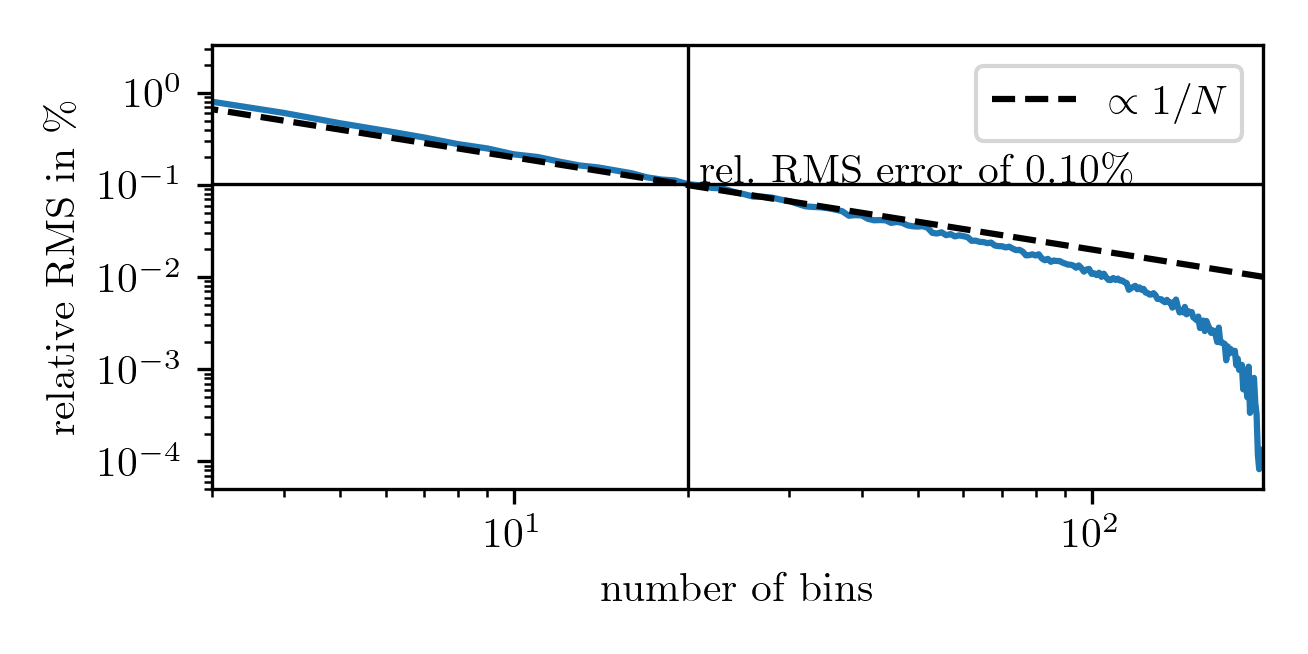
\includegraphics{relErrO3MeanVar.png}
	\caption[Relative Error of full posterior mean and covariance.]{Relative RMS error of $\bm{\mu}_{\bm{x}|\bm{y}}$ and covariance $\bm{\Sigma}_{\bm{x}|\bm{y}}$ calculated by the weighted expectations and compared to a ``ground truth'' given by weighted expectations over 200 bins.}
	\label{fig:MeanVarError}
\end{figure}
In Fig. \ref{fig:MeanVarError}, we plot the relative RMS error for the mean $\bm{\mu}_{\bm{x}|\bm{y}}$ and covariance $\bm{\Sigma}_{\bm{x}|\bm{y}}$ of $\pi(\bm{x}|\bm{y})$.
We obtain those results by calculating the weighted expectation over normalised histograms of $\pi(\lambda,\gamma | \bm{y})$, where we vary the number of bins and compare to a solution calculated from a histogram with 200 bins.
The relative error behaves roughly proportional to $1/N$, and we consider a relative error less than $0.5\%$ good enough, which we easily meet at 20 bins.
This sets the TT grid size and the number of evaluations of $\bm{x}_{\lambda}$ in Eq.~\ref{eq:MeanInt} and $(\gamma \bm{B}_{\lambda})^{-1}$ in Eq.~\ref{eq:CovInt}.
%marginal Ozone Pressure Temperature
\clearpage
%\subsubsection{Randomize then optimize -- RTO}
%For the RTO method we start by drawing an independent hyper-parameter sample $ ( \delta, \gamma) \sim \pi(\delta, \gamma | \bm{y})$ from the samples of the MwG.
%Then we generate two independent Gaussian random variables $\bm{v}_1 \sim \mathcal{N}(\bm{0},\gamma  \bm{A}^T_L \bm{A}_L)$ and $\bm{v}_2 \sim \mathcal{N}(\bm{0}, \delta \bm{L})$.
%Here  can use Cholesky factorisation of $\bm{L} =\bm{L}_C\bm{L}^T_C $ and the multiplication rule for normal distributions so that $\bm{v}_1 \sim \sqrt{\gamma} \bm{A}_L^T \mathcal{N}(0,\bm{I})$ and $\bm{v}_2 \sim \sqrt{\delta} \bm{L}_C \mathcal{N}(0,\bm{I})$.
%Then we solve
%\begin{align}
%	\label{eq:FirstRTO}
%	\left( \gamma \bm{A}_L^T  \bm{A}_L +\delta \bm{L} \right) \bm{x} = \gamma \bm{A}_L^T \bm{y} + \bm{v}_1 + \bm{v}_2 \, ,
%\end{align}
%using Cholesky back and forward substitution, for $\bm{x}$ and obtain one independent sample of $\pi(\bm{x}|\bm{y}, \bm{\theta})$.
%See Fig. \ref{fig:O3Samp}, where we plot $m = $ samples of the conditional posterior.
%
%The histogram in is binned as we intergate over it to 7 bins

\section{Approximate non-linear Forward Model with an Affine Map} 
\label{sec:affineMap}
Given the posterior distribution for ozone $ \pi(\bm{x}|\bm{y})$, we can now approximate the non-linear forward model 
\begin{align}
	\bm{A}(\bm{x}) \approx \bm{M A}_L \bm{x} \, ,
\end{align}
with an affine map $\bm{M}$ (see Fig.~\ref{fig:affinStrat} for the summarised strategy).
Here $\bm{A}(\bm{x})$ is non-linear noise-free data and $\bm{A}_L\bm{x}$ is linear noise-free data, both with ground truth pressure and temperature.
\begin{figure}[htb!]
	\centering
	\begin{tikzpicture}
		\node[rectnode] at (0,0) (Oy)    {$\bm{y}$};
		\node[roundnode2] at (0,-2) (x)     {$\bm{x}$};
		\node[rectnode] at (-1.75,-4) (NLy)    {$\bm{V}$};%{$\bm{A}_{NL}\bm{x}$};
		\node[rectnode] at (1.75,-4) (y)    {$\bm{W}$};%{$\bm{A}_L\bm{x}$};
		\draw[->, very thick] (Oy.south) -- (x.north); 
		\draw[->, very thick] (x.south west) -- (NLy.north); 
		\draw[->, very thick] (x.south east) -- (y.north); 
		\draw[->, very thick] (NLy.east) -- (y.west); 
		\node[align=center] at (1,0) (l1) {Data};
		\node[align=center] at (3.5,-2) (f2) {Ozone Profiles from $\pi(\bm{x}|\bm{y}) $};
		\node[align=center] at (1.75,-1) (l1) {$\pi(\lambda , \gamma  | \bm{y})$ with $\bm{A}_L$};
		
		
		\node[align=center] at (-4.75,-4) (f3) {non-linear forward model};
		\node[align=center] at (4.25,-4) (f4) {linear forward model};
		\node[align=center] at (0,-5) (f5) {$\bm{A}(\bm{x}) \approx \bm{M A}_L \bm{x}$ };
		
		\node[align=center] at (0,-4) (f5) {affine Map \\ $\bm{M}$};
		
	\end{tikzpicture}
	\caption[Strategy to find affine map.]{The strategy to find the affine map consists of first evaluating the marginal posterior for ozone $\pi(\lambda , \gamma  | \bm{y})$ based on the linear forward model. Then we draw ozone samples from the full posterior. Based on those ozone samples, we find an affine map which approximates between noise-free data from the linear and the non-linear forward model.}
	\label{fig:affinStrat}
\end{figure}


Using posterior ozone samples, we generate two affine subspaces and then find the mapping between those.
The subspace $\bm{W}$ is created by noise-free data based on the linear model and $\bm{V}$ by noise-free data based on the non-linear model, given $m$ samples $\bm{x}^{(j)} \sim \pi(\bm{x}|\bm{y})$ for $j = 1, \dots,m$.
We report a relative RMS difference between $\bm{W}$ and $\bm{V}$ of about $1\%$, which we aim to reduce through the affine map $\bm{M}$.
More specifically, the affine subspace associated with the linear forward model is 
\begin{align}
	\bm{W} = \begin{bmatrix}
		\vert&   &  \vert & & \vert \\
		\bm{A}_{L} \bm{x}^{(1)} &  \cdots& \bm{A}_{L} \bm{x}^{(j)} &  \cdots & \bm{A}_{L} \bm{x}^{(m)} \\
		\vert&   &  \vert & & \vert 
	\end{bmatrix}
	\in \mathbb{R}^{m \times m}
\end{align}\clearpage \noindent and with the non-linear forward model is 
\begin{align}
	\bm{V} = \begin{bmatrix}
		\vert&   &  \vert & & \vert \\
		\bm{A}(\bm{x}^{(1)}) &  \cdots& \bm{A}(\bm{x}^{(j)}) &  \cdots & \bm{A} (\bm{x}^{(m)})  \\
		\vert&   &  \vert & & \vert 
	\end{bmatrix} = 
	\begin{bmatrix}
		\begin{array}{ccc}
			\horzbar & v_{1} & \horzbar \\
			& \vdots    &          \\
			\horzbar & v_{j} & \horzbar \\
			& \vdots    &          \\
			\horzbar &v_{m} & \horzbar
		\end{array}
	\end{bmatrix}\in \mathbb{R}^{m \times m} \, .
\end{align}
Then we calculate the affine map 
\begin{align}
	\bm{V}\bm{W}^{-1} = \bm{M} =
	\begin{bmatrix}
		\begin{array}{ccc}
			\horzbar & r_{1} & \horzbar \\
			& \vdots    &          \\
			\horzbar & r_{j} & \horzbar \\
			& \vdots    &          \\
			\horzbar &r_{m} & \horzbar
		\end{array}
	\end{bmatrix}\, \in \mathbb{R}^{m \times m} .
\end{align}
by solving $v_j =r_j \bm{W}$ for each row $r_j$ in $\bm{M}$, where $j = 1, \dots, m$, using the Python function \texttt{numpy.linalg.solve}.
We can do that because every measurement in the data vector $\bm{y}$ is independent of each other, and then every row $v_j$ of $\bm{V} \in \mathbb{R}^{m \times m}$ is independent of each other as well.
%Alternatively, one can also determine this map using other methods, e.g. machine learning methods or matrix inversion, which in our case did not give better results.

We assess the affine map by calculating the relative RMS difference $\lVert \text{vec}(\bm{M}\bm{W}) - \text{vec}(\bm{V})  \rVert_{L^2} / \lVert \text{vec}(\bm{M}\bm{W}) \rVert_{L^2} $ between the mapped linear noise-free data and the non-linear noise-free data, which is approximately $0.001\%$.
\begin{figure}[t!]
	\centering
	%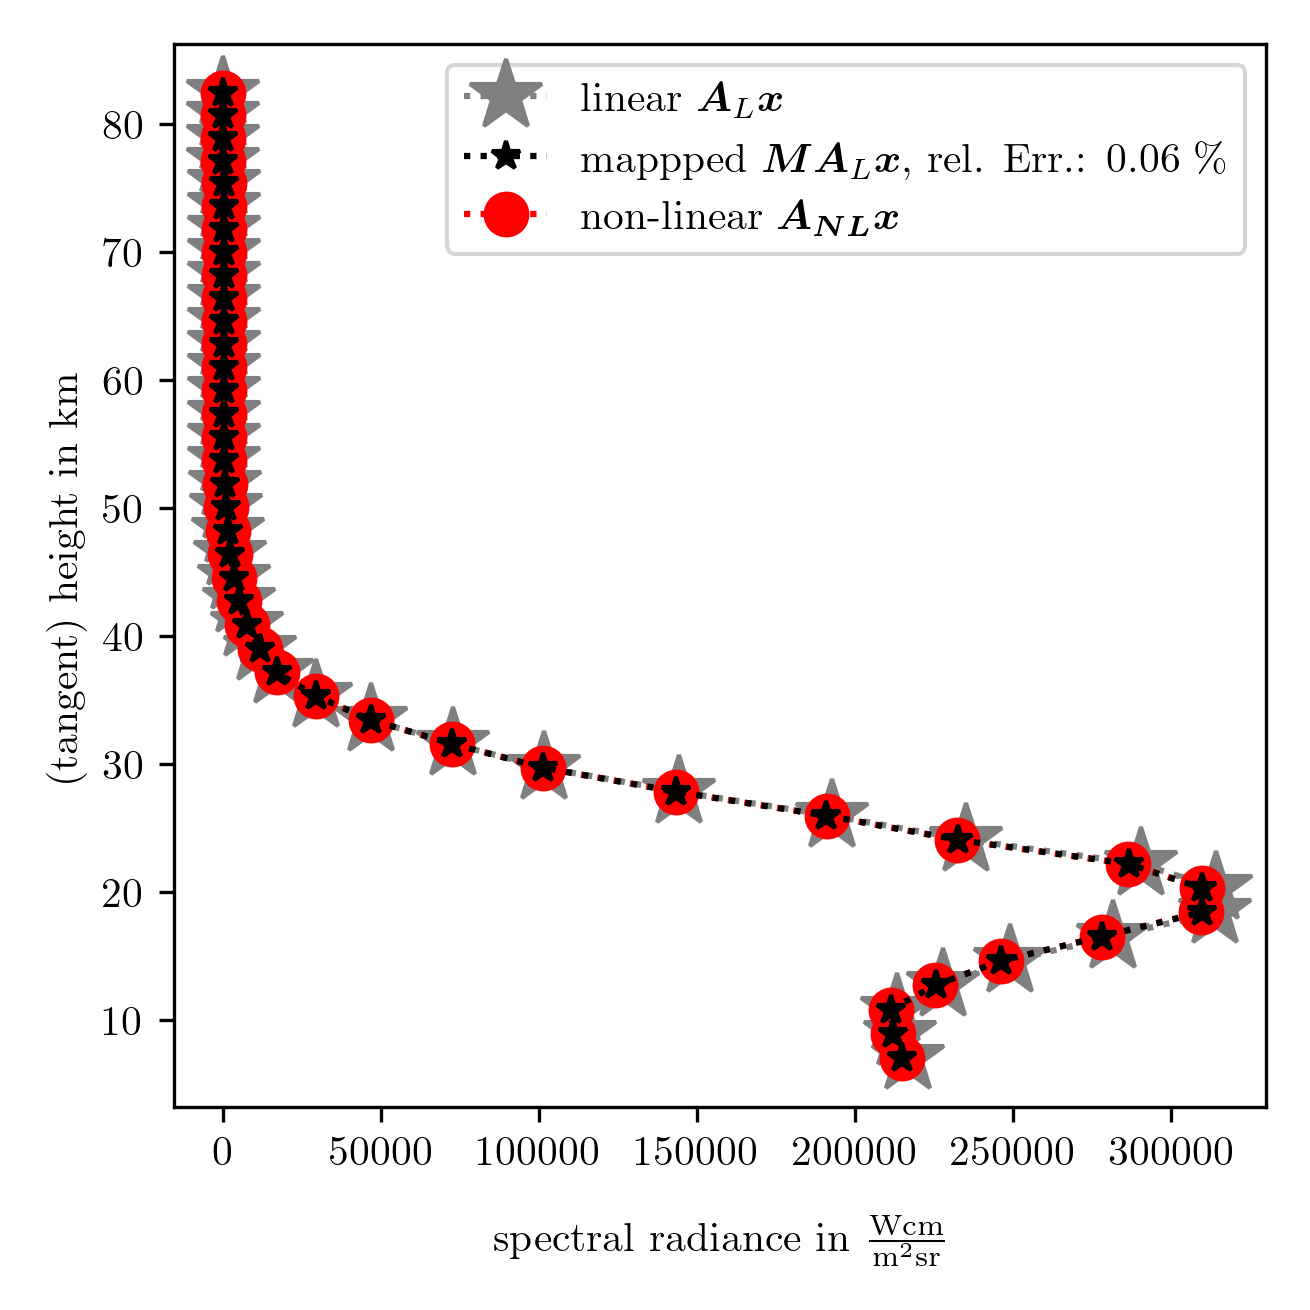
\includegraphics{SampMapAssesment.png}
	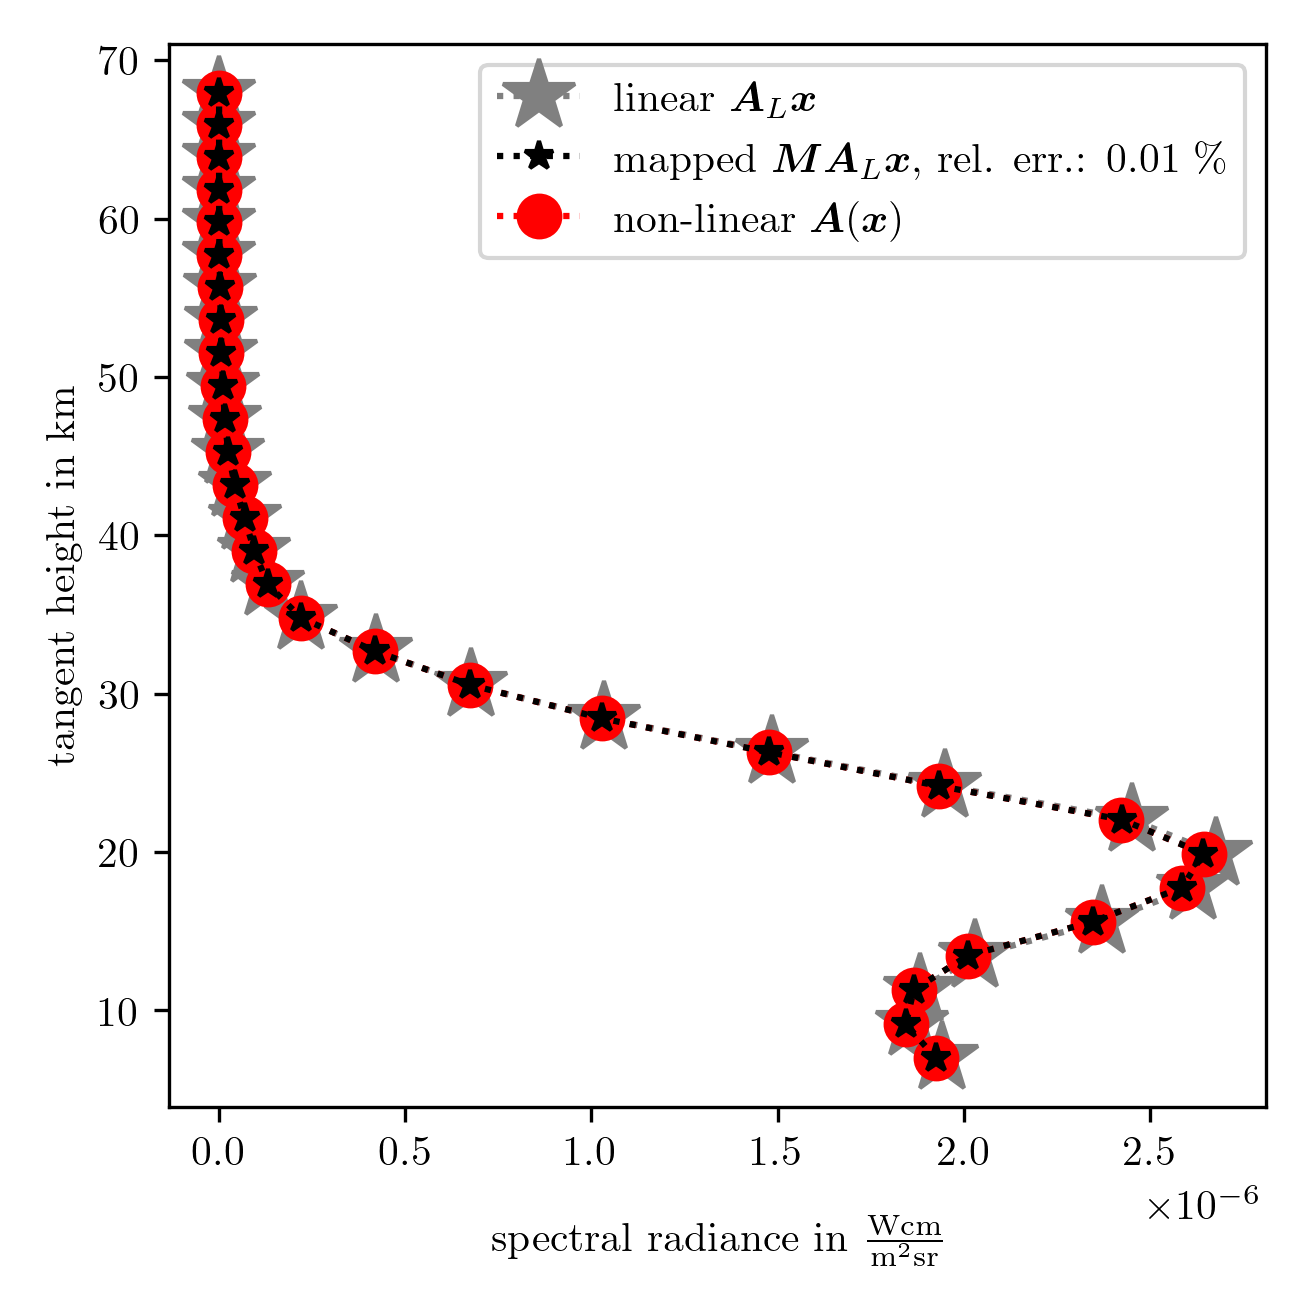
\includegraphics{SampMapAssesmentTT.png}
	\caption[Assessment of affine map.]{Assessment of how well we can approximate noise-free non-linear data $\bm{A}(\bm{x})$  (red circles) with noise-free linear data $\bm{A}_L\bm{x}$ (grey stars) and the previously calculated affine map $\bm{M}$. The approximated noise-free data (black stars) has a relative RMS error of $\approx 0.07\%$ compared to the true non-linear noise-free data.
	The ozone sample to generate this noise-free data has not been used to create the affine map.}
	\label{fig:MapAsses}
\end{figure}
In Fig.~\ref{fig:MapAsses}, we show the mapping for one posterior ozone sample, which has not been used to create this mapping.
In other words, this is an unseen event not occuring in the training data.
The relative RMS error for this approximation is roughly $0.07\%$ and much smaller than the relative difference between noise-free linear data and non-linear data.
Consequently, from here onwards, we use the approximated forward map.
\clearpage

\section{Regularisation Solution vs. Bayesian Approach -- Approximated Model}
\label{sec:ComparReg}%\section{Posterior Distribution of Ozone -- approximated Model}
With the affine approximation, we define the linear forward model matrix
\begin{align}
	\bm{A}  \coloneqq \bm{M A}_L \,
\end{align}
using the affine map $\bm{M}$.
Here, we compare the posterior distribution of ozone to a regularisation approach.

\subsection{Posterior Distribution for Ozone}
Again, we use the MTC scheme and the exact same setup and procedure as in Sec. \ref{sec:FirstO3Post} to evaluate the marginal posterior and then the full conditional posterior of ozone with similar computational time.

\begin{figure}[ht!]
	\centering
	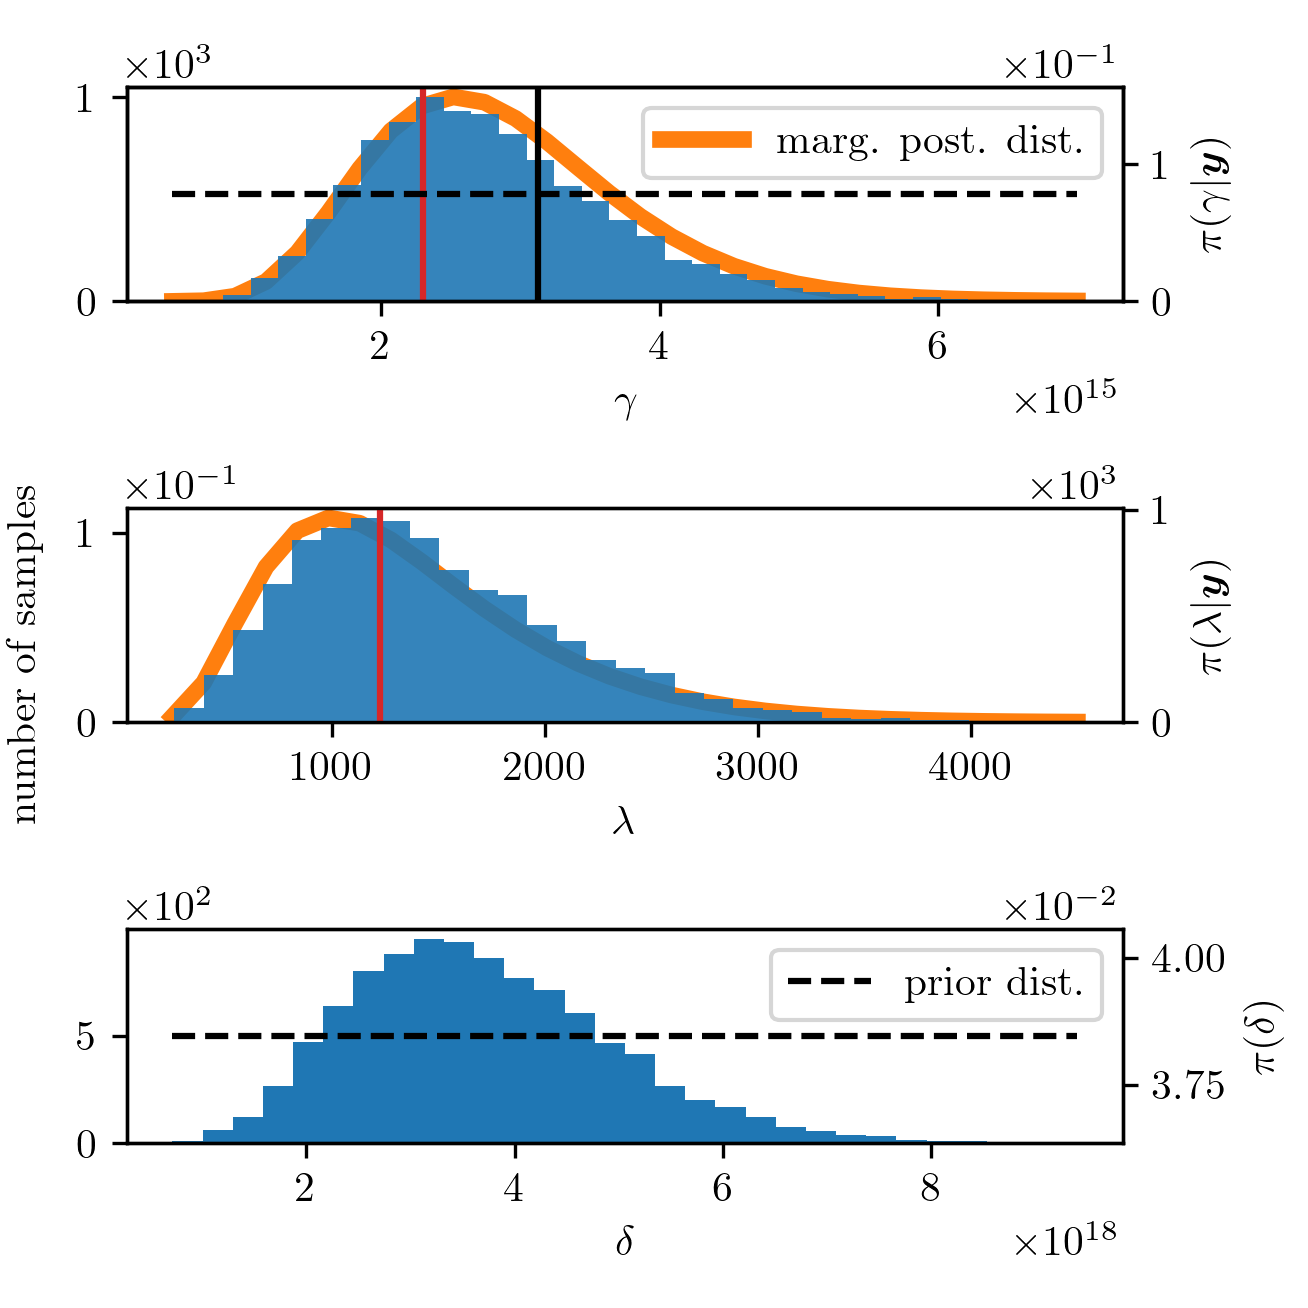
\includegraphics{secMargO3Res.png}
	\caption[Marginal posterior histograms and TT approximation as well as hyper-prior distribution.]{The TT approximation of the marginal posterior in orange and the samples as a histogram, as well as the prior distribution with a dotted line. We sample $\lambda$ and $\gamma$ using the MWG algorithm and then calculate $\delta$ for every sample of the marginal posterior. The regularised parameter corresponding to the best regularised solution (see Fig.~\ref{fig:O3SolplsReg} and Fig.~\ref{fig:LCurve}) is marked with the red vertical line. We mark the ground truth noise precision with the back vertical line.}
	\label{fig:MargPostHistTT}
\end{figure}
The marginal posterior is defined as in Eq.~\ref{eq:MargPostAppl}, but with the approximated forward model.
We initialise the MWG at and approximate $f(\lambda)$ and $g(\lambda)$ around the mode of $\pi(\lambda,\gamma| \bm{y})$ (see Eq.~\ref{eq:fAprox} and Eq.~\ref{eq:gAprox}), and take $N = 10000$ plus $N_{\text{burn-in}} = 100$ steps.
The IACTs provided by~\cite{drikHesse} are $\tau_{\text{int}, \gamma} \approx 4.0 \pm 0.2$ and $\tau_{\text{int}, \lambda} = 8.6 \pm 0.8 $ (see Fig. \ref{fig:IATCSecO3gam} and Fig.~\ref{fig:IATCSecO3lam}) and similar to the previously calculated values.
We plot the samples in Fig. \ref{fig:MargPostHistTT} as well as TT approximation of the marginal posterior using 400 function evaluations (same grid; same number of ranks; see Sec.~\ref{subsec:FirstMargPost}).
The approximation error of the TT is $\approx 3 \%$ and similar to the error due approximations of $f(\lambda)$ and $g(\lambda)$.

\begin{figure}[ht!]
	\centering
	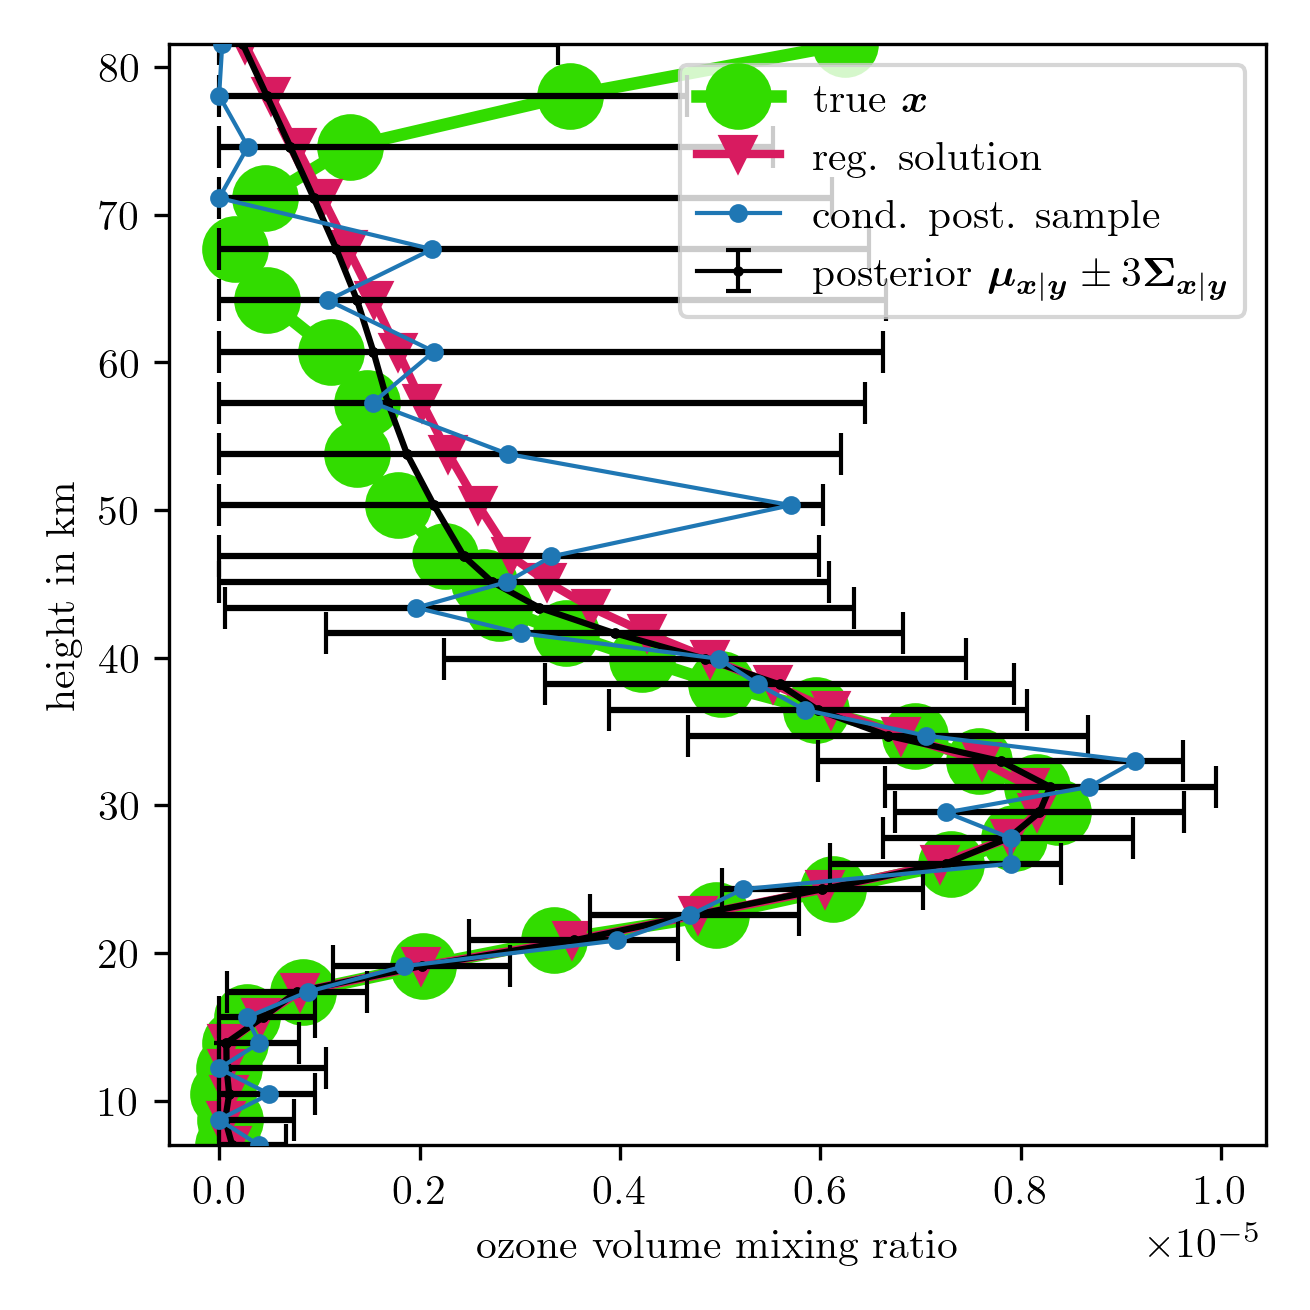
\includegraphics{SecRecResinclRegandSampl.png}
	%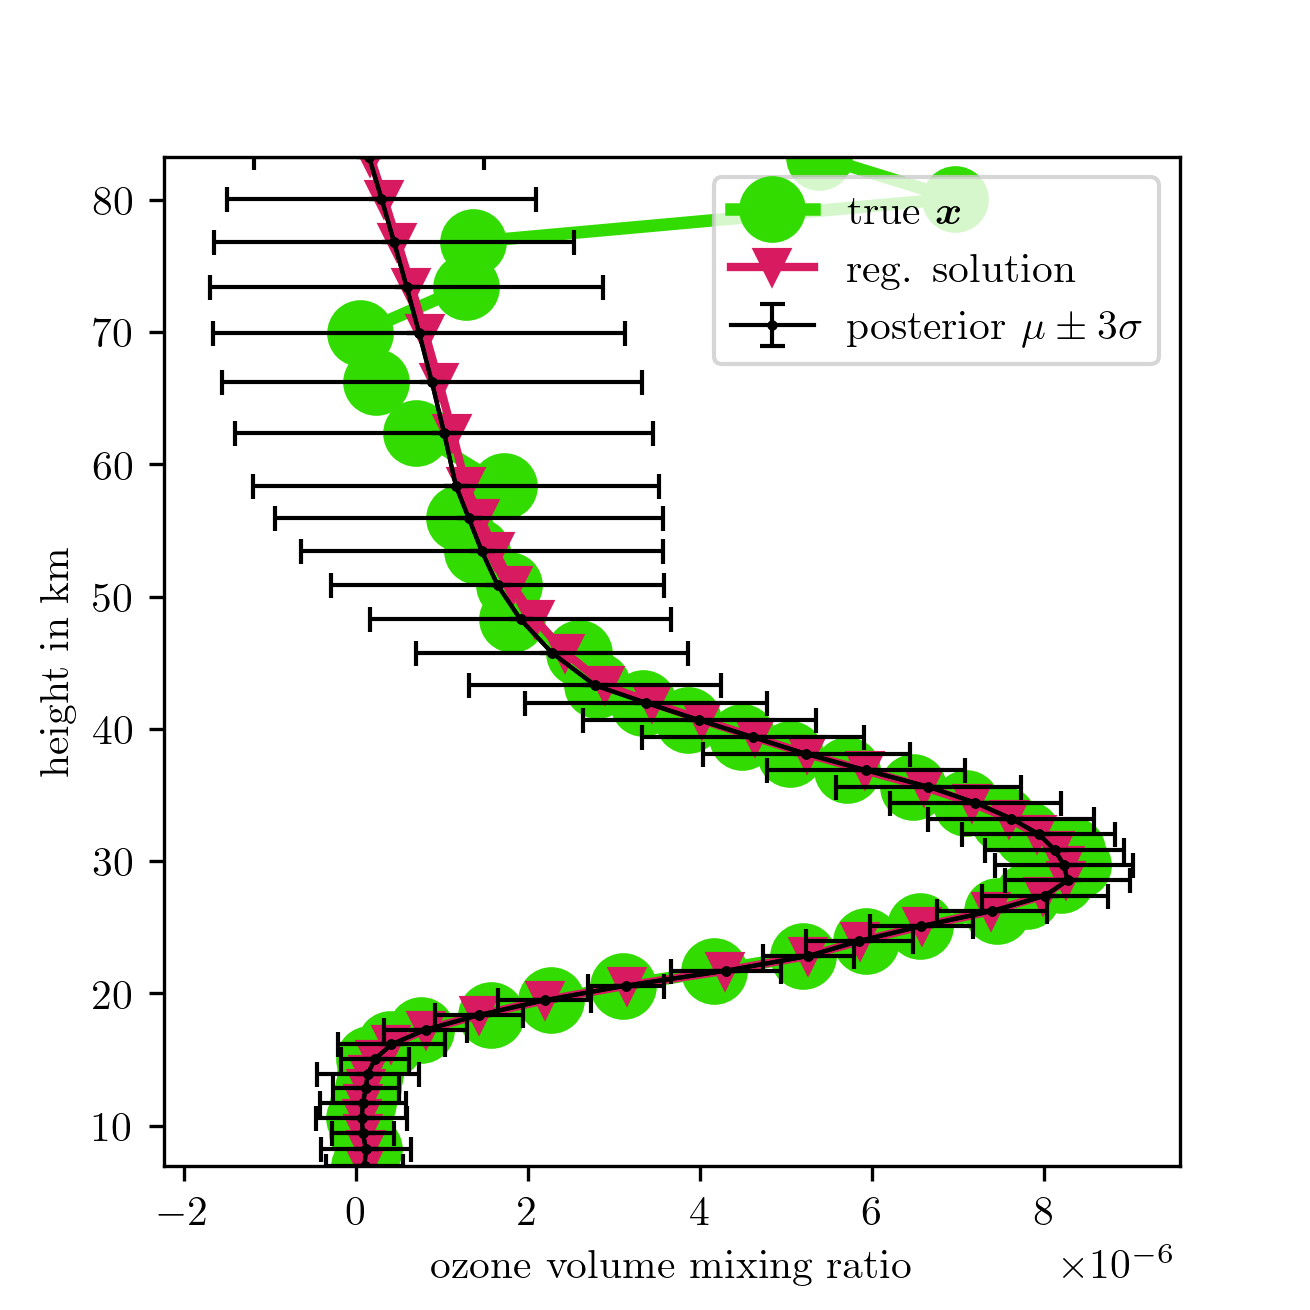
\includegraphics{SecRecResinclReg.png}
	\caption[Full posterior mean and variance of ozone and the regularised solution compared to the ground truth.]{Full  posterior mean and variance and one ozone sample from the full posterior. We plot the regularised solution on top of the ground truth ozone profile in green. The results are based on the approximated forward model $\bm{M}\bm{A}_L$.}
	\label{fig:O3SolplsReg}
\end{figure} 
Again, we calculate the full posterior mean $\bm{\mu}_{\bm{x}|\bm{y}}$, see Eq.~\ref{eq:MeanInt}, and covariance matrix $\bm{\Sigma}_{ \bm{x}|\bm{y}}$~\ref{eq:CovInt} as weighted expectation.
We plot the results and one sample of $\pi(\bm{x}|\bm{y})$, which represents a feasible solution to this inverse problem, in Fig.~\ref{fig:O3SolplsReg}, as well as the regularised solution (see next section), and one sample from the posterior.
We can see that the ground truth lies within three times of the STD (accounting for $\approx 99 \%$ of all posterior samples) around the mean, except for the peak at around $80$km.
Compared to the previously calculated mean and variance based on the linear forward model $\bm{A}_L$ (see \ref{fig:O3Samp}), the posterior distribution based on $\bm{M A}_L$ does not differ significantly.
This is expected since the difference between the linear and non-linear forward map of $\approx 1 \%$ is small.

\begin{figure}[ht!]
	\centering
	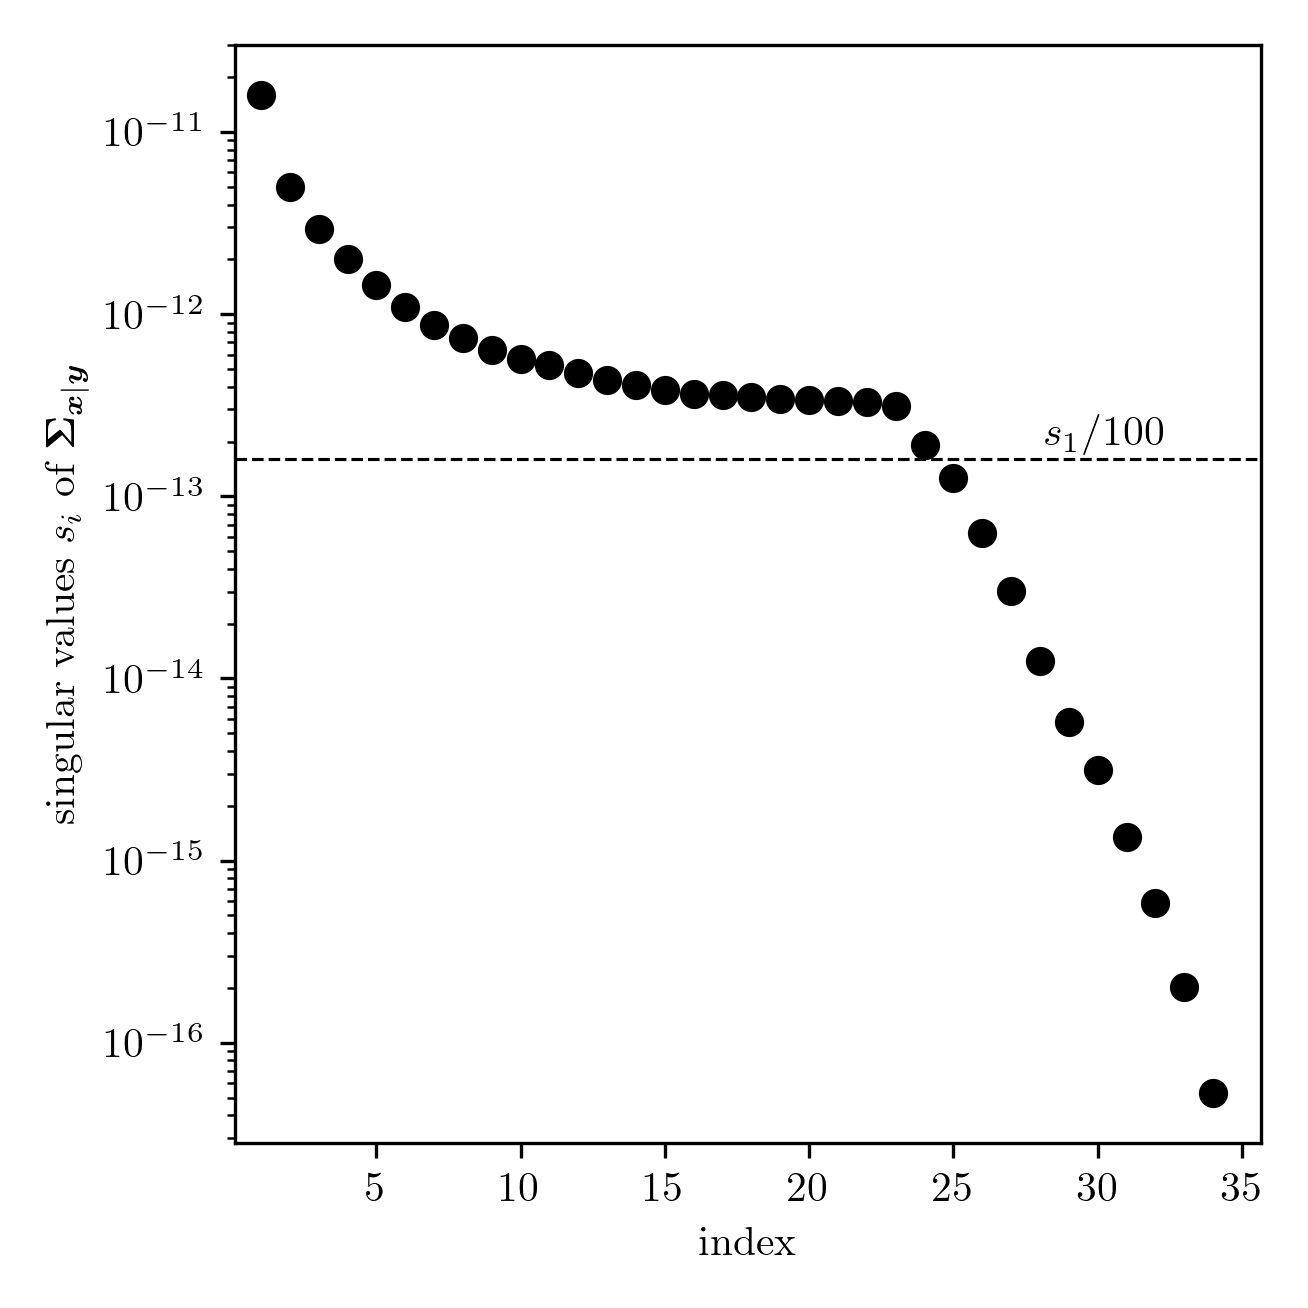
\includegraphics{CovSing.png}
	\caption[Eigenvalues of the posterior precision matrix]{Eigenvalues of the precision matrix of $\bm{Q}_{ \bm{x}|\delta, \gamma, \bm{y}}= \gamma \bm{A}^T \bm{A} + \delta \bm{L}$ of the full posterior distribution $\pi(\bm{x}|\delta, \gamma, \bm{y})$ for ozone.
	We see that large eigenvalues of $\gamma \bm{A}^T \bm{A}$ and $ \delta \bm{L}$ are rather unaffected by the prior compared to small eigenvalues.
The eigenbasis may differ.}
	\label{fig:PostCov}
\end{figure}
We can visualise how the posterior samples are affected through the prior $\delta \bm{L}$ and the forward model $\gamma \bm{A}^T \bm{A}$ by comparing their eigenvalues to the eigenvalues of the precision matrix $\bm{Q}_{ \bm{x}|\delta, \gamma,\bm{y}}=  \gamma \bm{A}^T \bm{A} + \delta \bm{L} $ for a random $\delta,\gamma \sim \pi(\delta,\gamma|\bm{y})$.
We order the eigenvalues in size and plot those in Fig.~\ref{fig:PostCov}.
We observe that the larger eigenvalues of $\bm{Q}_{ \bm{x}|\delta, \gamma,\bm{y}}$ are very much the same as the larger eigenvalues of $\gamma \bm{A}^T \bm{A}$.
Once the eigenvalues of $\gamma \bm{A}^T \bm{A}$ are significantly smaller than the eigenvalues of $\bm{Q}_{ \bm{x}|\delta, \gamma,\bm{y}}$ the structure of the eigenvalues is dominated by the eigenvalues of $\delta \bm{L}$.
The largest 10 eigenvalues of $\bm{Q}_{ \bm{x}|\delta, \gamma,\bm{y}}$ include ozone profile structure at lower altitudes, where the other eigenvector mainly represent structures at higher altitudes (see Fig.~\ref{fig:CovEigVec1} and Fig.~\ref{fig:CovEigVec1}).
Note that the eigenvalues of each matrix may correspond to different eigenvectors even if the eigenvalues of two matrices are the same.

\subsection{Solution by Regularisation}
\label{sec:reg}
Since we claim that the Bayesian approach is superior to regularisation methods, we compare the MTC method to a Tikhonov regularisation, see Sec.~\ref{sec:regularise} and~\cite{fox2016fast}.
This is most similar to our chosen linear-Gaussian Bayesian framework.

The regularised solution is defined as in~\cite{hansen2010discrete, fox2016fast} 
\begin{align}
	\bm{x}_{\lambda} =\underset{ \bm{x}}{\arg \min}\,  \lVert \bm{A}\bm{x} - \bm{y} \rVert_{L^2}^2 + \lambda \bm{x}^T \bm{L} \bm{x} \, ,
	\label{eq:XLam}
\end{align}
with the regularisation parameter $\lambda$,
and is typically calculated by solving the normal equations
\begin{align}
	\bm{x}_{\lambda} = (\bm{A}^T\bm{A} + \lambda \bm{L} )^{-1} \bm{A}^T \bm{y} \label{eq:xLam} \, 
\end{align}
(see Sec.~\ref{sec:regularise}).
To find the best regularised solution, we use the L-curve method, and follow~\cite{hansen1993use}.
Within this method we compute $\bm{x}_\lambda$, for 200 different $\lambda$ values in between $10^{0}$ to $10^{6}$ and plot the solution semi norm $\sqrt{\bm{x}_\lambda^T\mathbf{L} \bm{x}_\lambda}$ against the data misfit norm $\lVert \bm{A}\bm{x}_\lambda - \bm{x} \rVert_{L^2}$ (see Figure \ref{fig:LCurve}). 
The regularised solution corresponds to the ``corner'' of the L-curve at the point of maximum curvature provided by the kneedle algorithm~\cite{satopaa2011kneedle} using the function \texttt{kneed.KneeLocator} in $\approx 0.015$s, which is slightly faster then the TT approach to obtain full posterior mean and covariance.
We plot the corresponding regularisation parameter in Fig. \ref{fig:MargPostHistTT}, which can vary significantly compared to the $\lambda$-samples of the marginal posterior.
\begin{figure}[ht!]
	\centering
	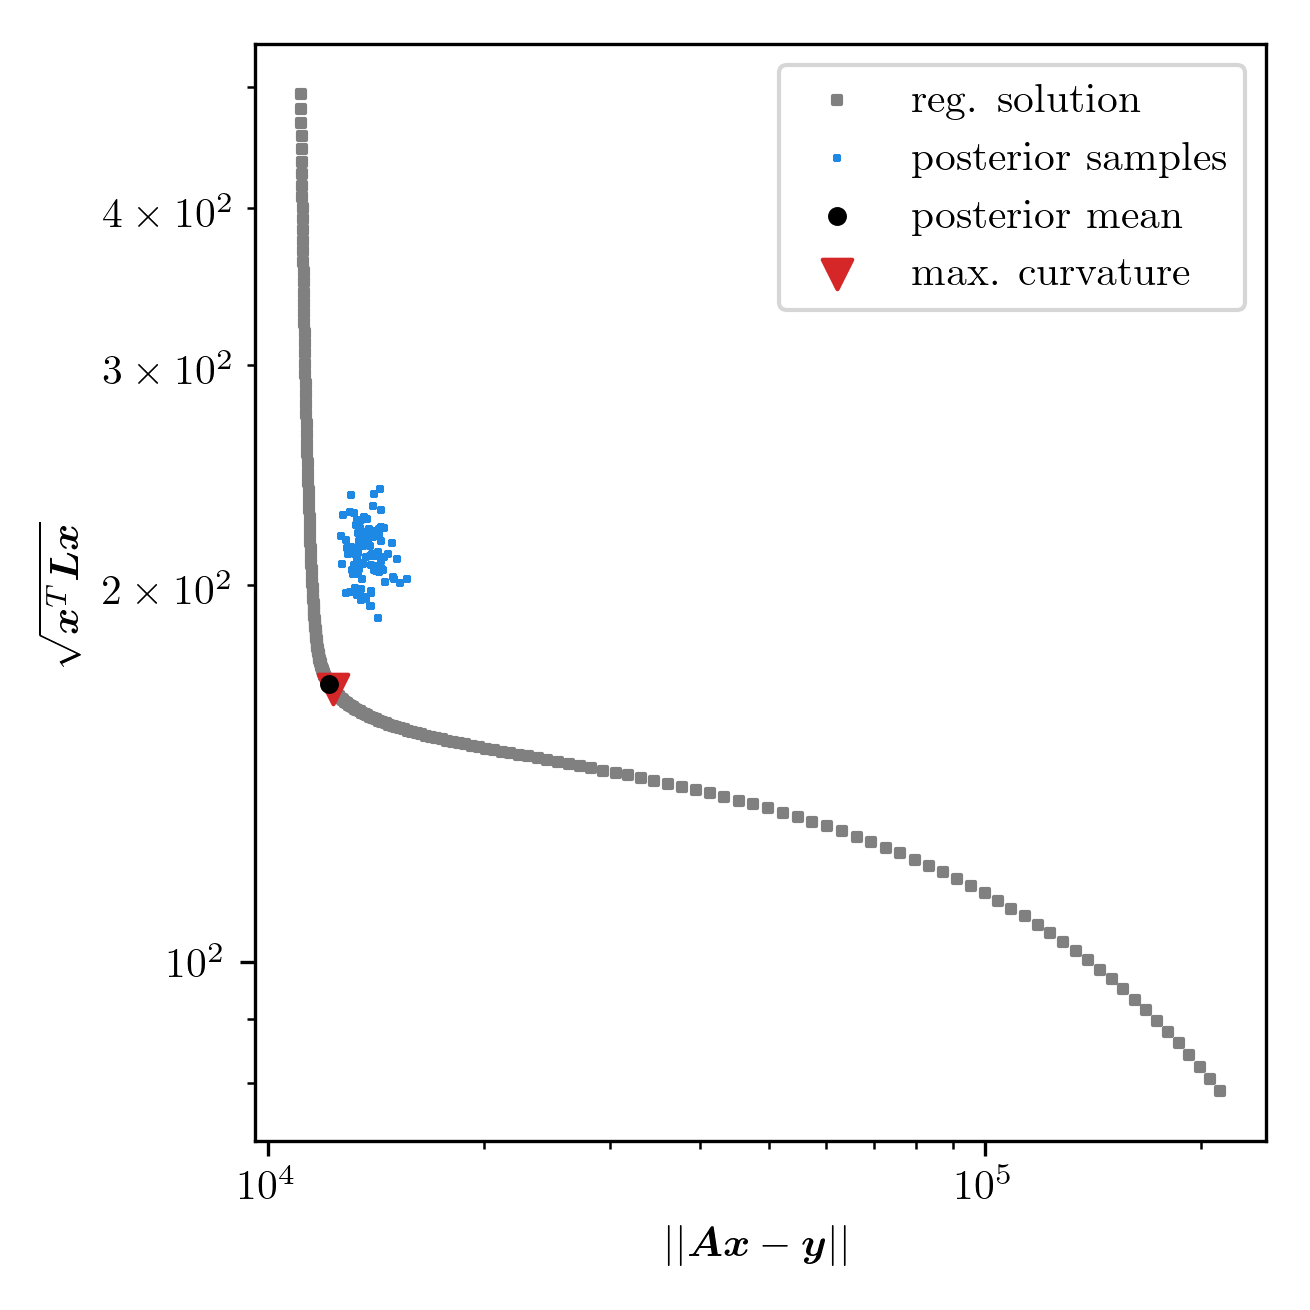
\includegraphics{LCurvePhD.png}
	\caption[Plot of the L-curve to find the regularised solution.]{L-Curve of regularised semi norm $\sqrt{\bm{x}^T\bm{Lx}}$ against the data misfit norm $\lVert \bm{A}\bm{x}_\lambda - \bm{x} \rVert_{L^2}$ for different $\lambda$ values, where $\bm{x}_{\lambda}$ is calculated as in Eq.~\ref{eq:xLam}. The best regularised solution is at the point of maximum curvature (pink triangle). Additionally, we calculate the data misfit norm and the regularised norm for the mean (black circle) and samples (blue squares) of the full posterior of ozone.}
	\label{fig:LCurve}
\end{figure}

The regularised solution in Fig.~\ref{fig:O3SolplsReg} is very similar to the posterior mean.
It is pretty clear that the regularised solution accounts for only one possible solution and does not provide uncertainties. The regularised solution is not similar to the samples drawn from the posterior $\pi(\bm{x}| \bm{y})$ (see Fig.~\ref{fig:O3Samp}).
The samples of $\pi(\bm{x}| \bm{y})$ plotted in Fig.~\ref{fig:LCurve} lie above the L-Curve, whereas the posterior mean and the regularised solution are on the L-Curve.
This does make sense, if one thinks about the mean as the (smooth) average over less-smooth samples and the regularised solution as an extremely smooth ozone profile (see Lagrange multiplier in Sec. \ref{sec:regularise}).
In contrast, the samples are less regularised and hence lie above the L-Curve, but have a similar data misfit norm, and as already mentioned, are all feasible solutions to the data.
Neither the regularisation solution nor the posterior ozone profiles capture the second ozone peak of the ground truth at high altitudes.
\clearpage

\section{Hierarchical Bayesian Framework for Ozone, Pressure and Temperature}
\label{sec:FullBay}
\begin{figure}[thb!]
	\centering
	\begin{tikzpicture}
		\node[roundnode2] at (-4.5,6.5) (Q)     {$\bm{Q}$};
		\node[roundnode2] at (-3,5) (x)     {$\bm{x}$};
		\node[align=center] at (-1,4) (A)    {$\bm{A}(\bm{\theta}_{\bm{p}, \bm{T}}) \coloneqq \bm{M}\bm{A}(\bm{\theta}_{\bm{p}, \bm{T}})_L$};
		\node[roundnode2] at (-1,2.5) (u)    {$\Omega$};
		\node[rectnode] at (-1,1) (y)    {$\bm{y}$};
		\node[roundnode2] at (-3,2.5) (e)    {$\bm{\eta}$};
		\node[roundnode2] at (-7.5,6.5) (S)    {$\bm{\Sigma}$};
		\node[roundnode2] at (-8.5,8) (s)    {$\gamma$};
		\node[roundnode2] at (-6,8) (d)    {$\delta$};
		\node[roundnode2] at (3,6.5) (t)     {$\bm{T}$};
		\node[roundnode2] at (-1,6.5) (p)     {$\bm{p}$};
		\node[roundnode2] at (1,5) (pt)     {$\bm{p}/\bm{T}$};
		\node[roundnode2] at (0,8) (b1)    {$b$};
		%\node[roundnode2] at (1,8) (b2)    {$b_2$};
		%\node[roundnode2] at (-2,8) (h1)    {$h_{0}$};
		\node[roundnode2] at (-1.5,8) (p0)    {$p_0$};
		\node[roundnode2] at (2.25,8) (ht)    {$\bm{h_T}$};
		\node[roundnode2] at (3.25,8) (ct)    {$T_0$};
		\node[roundnode2] at (4.25,8) (at)    {$\bm{a}$};
		
		\node[roundnode2] at (0,10) (b1hyp)    {$\bm{\theta}_{b}$};
		%\node[roundnode2] at (-2.5,10) (h1hyp)    {$\bm{\theta}_{h_{0}}$};
		\node[roundnode2] at (-1.5,10) (p0hyp)    {$\bm{\theta}_{p_{0}}$};
		\node[roundnode2] at (2,10) (hthyp)    {$\bm{\theta}_{\bm{h}_T}$};
		\node[roundnode2] at (3.25,10) (cthyp)    {$\bm{\theta}_{T_{0}}$};
		\node[roundnode2] at (4.5,10) (athyp)    {$\bm{\theta}_{\bm{a}}$};
		
		\node[roundnode2] at (-8.5,10) (shyp)    {$\bm{\theta}_{\gamma}$};
		\node[roundnode2] at (-6,10) (dhyp)    {$\bm{\theta}_{\delta}$};
		
		%Lines
		
		
		\draw[->, very thick] (S) -- (e);
		\draw[->, mydotted, very thick] (s) -- (S);
		\draw[->, very thick] (u) -- (y);
		\draw[->, mydotted, very thick] (A) -- (u);
		\draw[->, mydotted,  very thick] (x) -- (A);
		\draw[->, mydotted, very thick] (p) -- (pt);
		\draw[->, mydotted, very thick] (t) -- (pt);
		\draw[->, mydotted, very thick] (pt) -- (A);
		%\draw[->, mydotted, very thick] (h1) -- (p);
		\draw[->, mydotted, very thick] (p0) -- (p);
		\draw[->, mydotted, very thick] (b1) -- (p); 
		%\draw[->, very thick] (b2.south) -- (p.east); 
		\draw[->, mydotted, very thick] (d) -- (Q); 
		\draw[->, mydotted, very thick] (e) -- (y); 
		
		\draw[->, very thick] (Q.south east) -- (x.north west); 
		\draw[->, mydotted, very thick] (ht.south) -- (t.north west);
		\draw[->, mydotted, very thick] (ct.south) -- (t.north);
		\draw[->, mydotted, very thick] (at.south) -- (t.north east);
		
		
		\draw[->, very thick] (b1hyp) -- (b1);
		%\draw[->, very thick] (h1hyp) -- (h1);
		\draw[->, very thick] (p0hyp) -- (p0);
		\draw[->, very thick] (hthyp) -- (ht);
		\draw[->, very thick] (cthyp) -- (ct);
		\draw[->, very thick] (athyp) -- (at);
		\draw[->, very thick] (shyp) -- (s);
		\draw[->, very thick] (dhyp) -- (d);
		
		\node[fit=(s)(at),draw,dotted,black, rounded corners] {};
		\node[align =center] at (-3.75,8) (T1) {hyper-parameters};
		\node[align =center] at (-4.5,5) (T2) {parameter};
		\node[fit=(x)(T2),draw,dotted,black, rounded corners] {};
		
	\end{tikzpicture} 
	\caption[Directed acyclic graph of Bayesian model for ozone, pressure and temperature.]{DAG of Bayesian model for ozone, pressure and temperature. The hyper-parameters $\bm{h}_T= \{ h_{T,1}, h_{T,2},h_{T,3},h_{T,4},h_{T,5},h_{T,6}\}$, $\bm{a} = \{ a_0, a_1, a_2,a_3,a_4,a_5,a_6\}$, $T_0$, $b$ and $p_0$ deterministically (dotted line) describe pressure parameter $\bm{p}$ through the function in Eq.~\ref{eq:pressFunc}, and temperature parameter $\bm{T}$ through the function in Eq.~\ref{eq:tempFunc}. In this case, we choose the hyper-parameters $\pi(p_0,b,T_0,\bm{h_T},\bm{a})$ to be a normally distributed apriori, determined by $\bm{\theta}_{\bm{h}_T},\bm{\theta}_{\bm{a}}, \bm{\theta}_{T_{0}},\bm{\theta}_{b} , \bm{\theta}_{p_0}$, which represent mean and variances. 
	The ozone parameter $\bm{x}$ is statistically (solid line) described by the prior distribution $\bm{x}| \delta \sim \mathcal{N}(0,(\delta \bm{L})^{-1}) $. 
	Here, the hyper-parameter $\delta$ accounts for smoothness in the ozone profile and defines the precision matrix $\bm{Q} = \delta \bm{L}$, where $\bm{L}$ is the graph Laplacian as in Eq. \ref{eq:GLapl}.
	The noise covariance $\bm{\Sigma} = \gamma^{-1} \bm{I}$ of the random noise vector $\bm{\eta} \sim \mathcal{N}(0,\gamma^{-1} \bm{I} ) $ is defined by the noise hyper-parameter $\gamma$.
	As in Sec. \ref{sec:BayModelO3} described, $\bm{\theta}_{\delta}$ and $\bm{\theta}_{\gamma}$ define the hyper-priors $\pi(\delta, \gamma)$.
	Then, we randomly observe a data set $\bm{y}$ from the space of all measurables $\Omega$ through the approximated forward model $\bm{A}(\bm{\theta}_{\bm{p}, \bm{T}}) \coloneqq \bm{M}\bm{A}(\bm{\theta}_{\bm{p}, \bm{T}})_L$, depending on the hyper-parameter $\bm{\theta}_{\bm{p}, \bm{T}}  \coloneqq \{p_0, b, \bm{h}_T, \bm{T}_0, \bm{a} \}$, including some added noise.
	Given the data we like to determine the posterior distribution over the hyper-parameters $\pi(p_0,b,T_0,\bm{h_T},\bm{a}, \delta, \gamma | \bm{y})$ first and then $\pi(\bm{x}|p_0,b,T_0,\bm{h_T},\bm{a}, \delta, \gamma, \bm{y})$, utilising the MTC scheme.}
	\label{fig:DAGComplete}
\end{figure}

As in Sec. \ref{sec:BayModelO3}, we use a DAG as in Fig.~\ref{fig:DAGComplete} to visualise the measurement process and correlations between pressure $\bm{p}$, temperature $\bm{T}$ and ozone $\bm{x}$, which progress deterministically (dashed line) into the forward model, via $\bm{x} \times \bm{p} / \bm{T}$.
Note that other variables such as absorption constant, internal partition function and the black body radiation are also dependent on temperature.
Through their respective prior distributions, they generate a space of all possible noise-free data $\Omega$, from which we observe some data, including some added normally distributed noise $\bm{\eta}$.
This hierarchical Bayesian framework includes the hyper-parameters $p_0, b $ for pressure (see Eq.~\ref{eq:pressFunc}), $\bm{a}, \bm{h}_T, T_0$ for temperature (see Eq.~\ref{eq:tempFunc}), $\delta$ for ozone smoothness and $\gamma$ for noise precision.
Each of those hyper-parameters is described by the hyper-prior distribution $\pi(p_0,b,T_0,\bm{h_T},\bm{a}, \delta,\gamma)$ defined by us.
Here $\bm{\theta}_{\gamma}, \bm{\theta}_{\delta}$ determine gamma distributions, e.g. $\gamma \sim \Gamma(\alpha_{\gamma},\beta_{\gamma}) $ with $\bm{\theta}_{\gamma} = \{\alpha_{\gamma},\beta_{\gamma} \}$, and $\bm{\theta}_{p_0},\bm{\theta}_{b},\bm{\theta}_{\bm{h}},\bm{\theta}_{T_0},\bm{\theta}_{\bm{a}}$ determine a normal distribution $p_0, b, \bm{h}_T, \bm{T}_0, \bm{a} \sim \pi( \bm{\theta}_{p_0},\bm{\theta}_{b},\bm{\theta}_{\bm{h}},\bm{\theta}_{T_0},\bm{\theta}_{\bm{a}})$, e.g. $b \sim \mathcal{N}(\mu_b, \sigma^2_b)$ and $\bm{\theta}_{b} = \{\mu_b, \sigma_b\}$.
We use the approximated forward model $\bm{A}(\bm{\theta}_{\bm{p}, \bm{T}}) \coloneqq \bm{M}\bm{A}(\bm{\theta}_{\bm{p}, \bm{T}})_L$ and denote $\bm{\theta}_{\bm{p}, \bm{T}}  \coloneqq \{p_0,b,T_0,\bm{h_T},\bm{a} , \}$, which includes all hyper-parameter related to pressure and temperature.
\begin{table}
	\centering
	\begin{tabular}{ |c||c|c|c|c|c|   }
		\hline
		& &\multicolumn{2}{|c|}{TT bounds}& &\\
		\hline
		model parameters& priors&\makecell{lower}& \makecell{upper\\
		}&$\tau_{\text{int}}$&Context\\
		\hhline{|=||=|=|=|=|=|}
		$\bm{x}$ &$\mathcal{N}(0,(\delta \bm{L})^{-1})$ & -&-&-& $\bm{x}$\\ \hline
		$\delta$ &$\mathcal{T}(1,10^{-35})$ & -&-&  & $\bm{x}$\\ \hline
		$\gamma$ & $\mathcal{T}(1,10^{-35})$ &$2.5\,10^{14}$ &$6\,10^{15}$&  $ 512\pm 30$ &$\bm{y}$\\ \hline
		$\lambda  = \delta / \gamma$ &- & 1&$2\,10^{4}$& $976 \pm 74$ &$\bm{x}$\\ \hline
		$b$ &  $\mathcal{N}(0.174,(0.01)^2)$& 0.129& 0.214 &$864\pm 62$&$\bm{p}$\\ \hline
		$h_{T,1}$ &  $\mathcal{N}(11,(1.5)^2)$&5.4 &16.3&$270\pm 12$ &$\bm{T}$\\ \hline
		$T_{0}$ &  $\mathcal{N}(288.15,(10)^2)$& 247 &326&$304 \pm 14$&$\bm{T}$\\ \hline
		$p_0$ &  $\mathcal{N}(1311,(20)^2)$&1237 &1387&$252\pm 10$&$\bm{p}$\\ \hline
		$h_{T,3}$ &  $\mathcal{N}(32.3,(2.5)^2)$&22.9&41.7&$272 \pm 12$&$\bm{T}$\\ \hline
		$a_{1}$ &  $\mathcal{N}(0,(0.1)^2)$&-0.38 &0.38&$248 \pm 10$&$\bm{T}$\\ \hline
		$h_{T,2}$ &  $\mathcal{N}(20.1,(0.7)^2)$&17.2 &22.7&$268\pm 10$&$\bm{T}$\\ \hline
		$a_{0}$ &  $\mathcal{N}(-6.5,(0.01)^2)$&-6.54 &-6.47&$250 \pm 10$&$\bm{T}$\\ \hline
		$a_{2}$ &  $\mathcal{N}(1,(0.01)^2)$&0.97 &1.03&$258 \pm 10$&$\bm{T}$\\ \hline
		$a_{3}$ &  $\mathcal{N}(2.8,(0.1)^2)$&2.5 &3.1&$254\pm 10$&$\bm{T}$\\ \hline
		$h_{T,4}$ &  $\mathcal{N}(47.4,(0.5)^2)$&45.5 &49.3&$252 \pm 10$&$\bm{T}$\\ \hline
		$a_{4}$ &  $\mathcal{N}(0,(0.1)^2)$&-0.38 &0.38&$274 \pm 12$&$\bm{T}$\\ \hline
		$h_{T,5}$ &  $\mathcal{N}(51.4,(0.5)^2)$&49.5 &53.3&$274 \pm 12$&$\bm{T}$\\ \hline
		$a_{5}$ &  $\mathcal{N}(-2.8,(0.1)^2)$&-3.18 &-2.43&$264 \pm 10$&$\bm{T}$\\ \hline
		$h_{T,6}$ &  $\mathcal{N}(71.8,(3)^2)$&60.5 &83.1&$264\pm 10$&$\bm{T}$\\ \hline
		$a_{6}$ & $\mathcal{N}(-2,(0.01)^2)$ &-2.04 &-1.96&$262\pm 10$&$\bm{T}$\\
		\hline
	\end{tabular}
	\caption[Summary of relevant parameter characteristics, bounds and sampling statistics.]{\textcolor{red}{Summary of relevant parameter characteristics, bounds and sampling statistics. We denote $\mathcal{N}(\mu,\sigma^2)$ as the Gaussian and $\mathcal{T}(\alpha = \text{scale}, \beta = \text{rate})$ as the gamma distribution. The IACT $\tau_{\text{int}}$ is estimated as in~\cite{UwerrM} from posterior samples based on the approximated forward map.}}
	\label{tab:priors}
\end{table}

Then, we set up the hierarchical Bayesian framework
\begin{subequations}
	\begin{align}
		\bm{y} |  \bm{x},p_0,b,T_0,\bm{h_T},\bm{a} ,\delta,\gamma  &\sim \mathcal{N}(\bm{A}(p_0,b,T_0,\bm{h_T},\bm{a}) \, \bm{x}, \gamma^{-1} \bm{I}) \label{eq:likelihoodFull} \\
		\bm{x}| \delta  &\sim \mathcal{N}(\bm{0}, (\delta \bm{L})^{-1} ) \label{eq:priorXFull} \\
		\delta  &\sim \Gamma(\alpha_{\delta} , \beta_{\delta} )\label{eq:priorDelFull} \\
		\gamma  &\sim \Gamma(\alpha_{\gamma}, \beta_{\gamma})\label{eq:priorGamFull} \\
		\bm{a}  &\sim \mathcal{N}(\bm{\mu}_{\bm{a}}, \bm{\Sigma}_{\bm{a}})\\
		\bm{h}_{\bm{T}}  &\sim \mathcal{N}(\bm{\mu}_{T}, \bm{\Sigma}_{\bm{h}_T}) \\
		T_0  &\sim \mathcal{N}(\mu_{T_0}, \sigma_{T_0} )\\
		p_0  &\sim \mathcal{N}(\mu_{p_0}, \sigma_{p_0} )\\
		b  &\sim \mathcal{N}(\mu_b, \sigma_b )
	\end{align}
	\label{eq:BayMode}
\end{subequations}
and define a normally distributed likelihood (due to Gaussian noise) and normally distributed priors.
Before we formulate the posterior distribution, we carefully define $\bm{\theta}_{\gamma}, \bm{\theta}_{\delta},\bm{\theta}_{p_0},\bm{\theta}_{b},\bm{\theta}_{\bm{h}},\bm{\theta}_{T_0},\bm{\theta}_{\bm{a}}$, the hyper-prior scales, shapes, means and variances, which are explicitly given in Tab.~\ref{tab:priors}.

\subsection{Prior Modelling}
\begin{figure}[ht!]
	\centering
	\input{TrueTemp.pdf_tex}
	%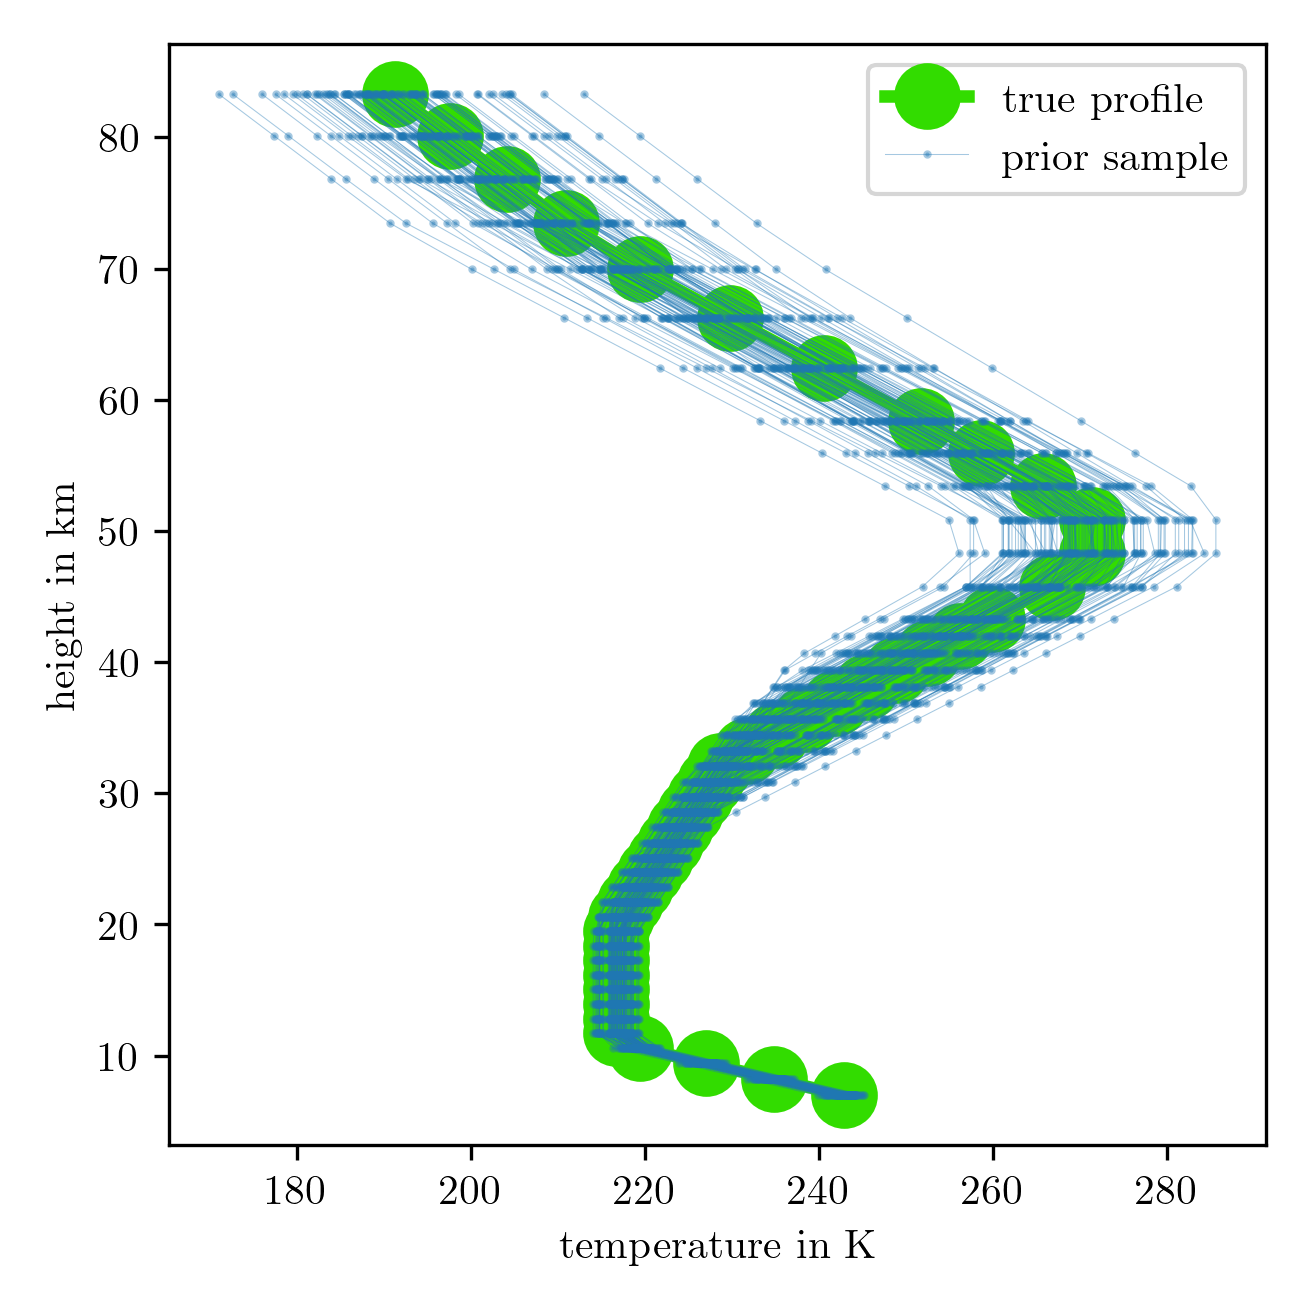
\includegraphics{PriorTempPostMeanSigm.png}
	\caption[Prior Samples of $\bm{T}$ according to the respective hyper-prior distribution.]{Prior samples from the hyper-prior distribution of $\bm{h}_T$, $\bm{a}$ and $T_0$, as defined in Tab.~\ref{tab:priors}, where we calculate $\bm{T}$ according to the function in Eq.~\ref{eq:tempFunc}.}
	\label{fig:PriorTemp}
\end{figure}

\begin{figure}[ht!]
	\centering
	\input{TruePress.pdf_tex}
	%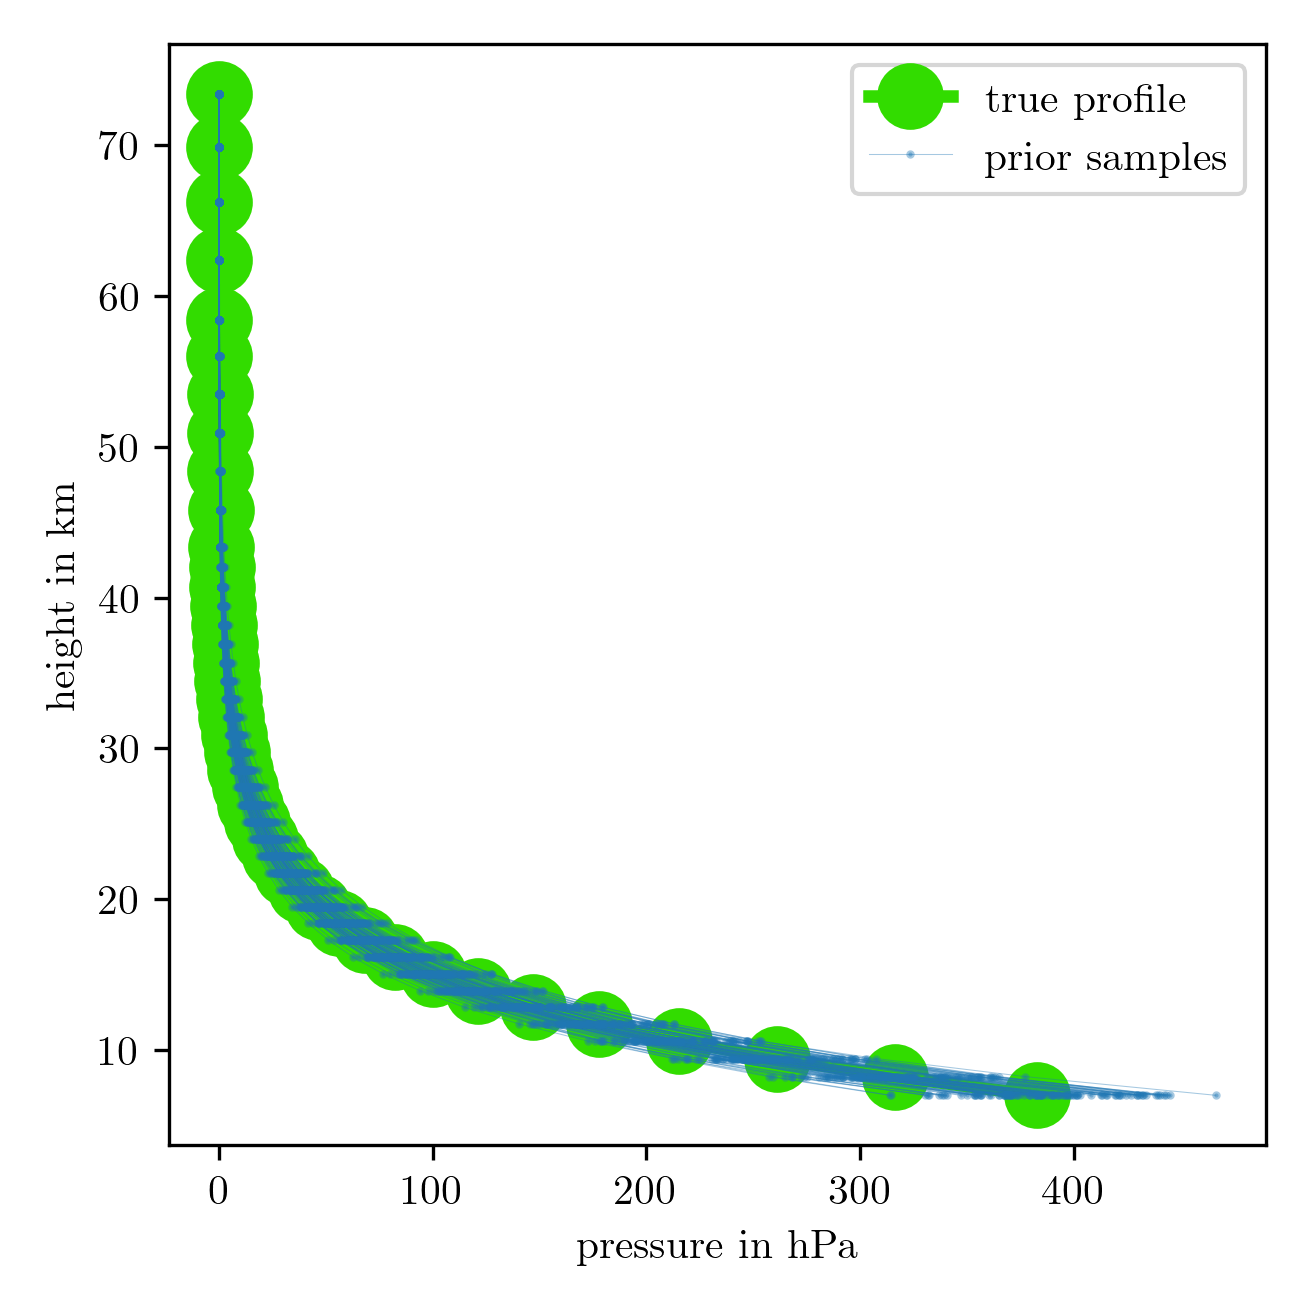
\includegraphics{PriorPressPostMeanSigm.png}
	\caption[Prior Samples of $\bm{p}$ according to the respective hyper-prior distribution.]{Prior samples from the hyper-prior distribution of $b$ and $p_0$ as defined in Tab.~\ref{tab:priors}, where we calculate $\bm{p}$ according to the function in Eq.~\ref{eq:pressFunc}.}
	\label{fig:PriorPress}
\end{figure}
\begin{figure}[ht!]
	\centering
	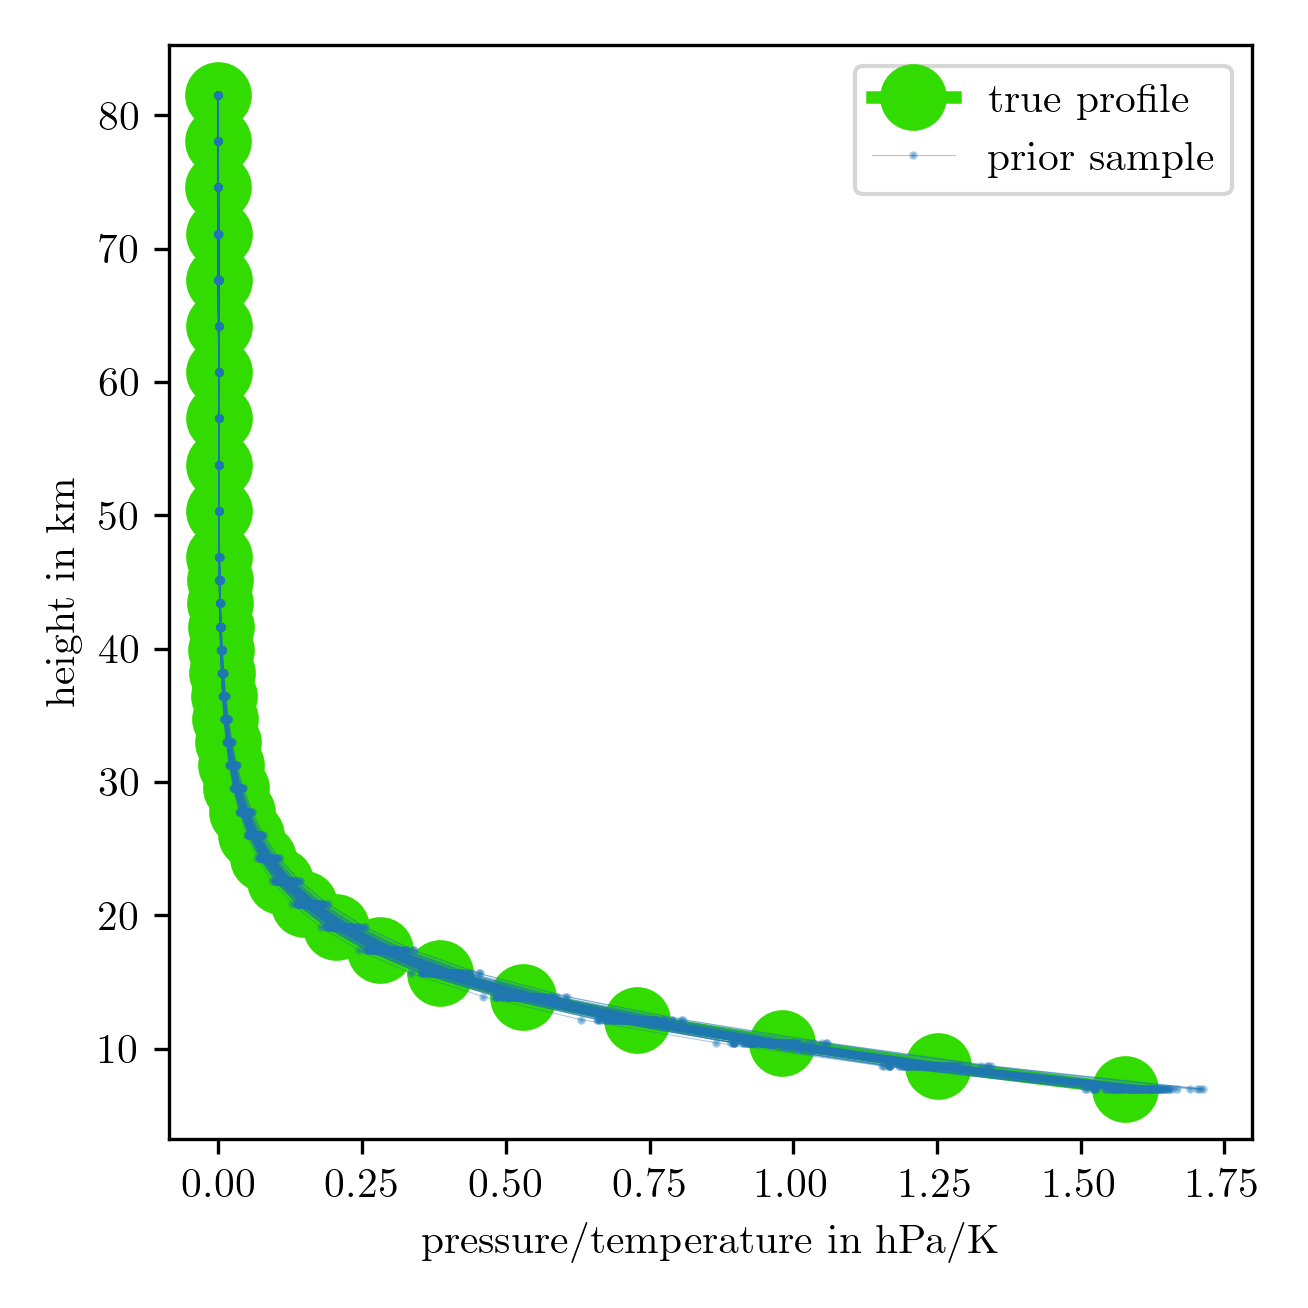
\includegraphics{PriorTempOverPostMeanSigm.png}
	\caption[Prior Samples of $\bm{p}/\bm{T}$ according to the respective hyper-prior distribution.]{Prior samples from the hyper-prior distribution of $\bm{h}_T$, $\bm{a}$ and $T_0$ for temperature as in Eq.~\ref{eq:tempFunc} and $b$ and $p_0$ for pressure as in Eq.~\ref{eq:pressFunc}. We plot $\bm{p}/\bm{T}$. The hyper-priors are defined in Tab.~\ref{tab:priors}.}
	\label{fig:PriorPressOverTemp}
\end{figure}
We start by describing the pressure $\bm{p}$ in between $h_{L,0} \approx 7$km and $h_{L,n} \approx 82$km with an exponential function
\begin{align}
	p(h) =
	\exp \left( -b \, h \right)   \,  p_0 \quad , \text{$h_{L,0}  \leq h \leq h_{L,n}$}
	\label{eq:pressFunc}
\end{align}
depending on two hyper-parameters $p_0,b$, see Fig.~\ref{fig:PriorPress}.
Similarly, the temperature as described in Eq.~\ref{eq:tempFunc} can be parametrised with 14 hyper-parameters\linebreak $\bm{h}_T = \{ h_{T,1}, h_{T,2},h_{T,3},h_{T,4},h_{T,5},h_{T,6} \}$, $\bm{a} = \{a_0, a_1, a_2,a_3,a_4,a_5,a_6 \} $ and $T_0$ (see Fig.~\ref{fig:PriorTemp} and Eq.~\ref{eq:tempFunc}).
To complete the model, we have to define sensible hyper-prior variances and means of the normally distributed hyper-prior distribution for pressure and temperature-related hyper-parameters, where $\pi(\delta,\gamma)$ are the same gamma distributions as previously defined in Sec.~\ref{subsec:PriorModelO3}.
We tune the normal distribution $\pi(\bm{h}_T)$, so that the temperature profile maintains its structure, $ h_{T, i} < h_{T, i+1}$ for $i = 1,\dots, 5$ (see Fig.~\ref{fig:HeightPriors}) and set $\pi(\bm{a})$ to a normal distribution as well.
Similarly, we set $\pi(T_0)$ to a normal distribution, so that it mimics a daily temperature variability of roughly 30K.
We choose those rather informative hyper-prior distributions, because we find (see Fig.~\ref{fig:PriorPressOverTemp}) that the data is uninformative about the temperature profile.
The hyper-prior distribution $\pi(p_0, b)$ for pressure-related hyper-parameters is also normally distributed, but with rather large variance $\sigma^2_b$, where $p_0$ has a variability of around 80hPa, close to what we can observe when looking at weather data.
%Note that we fit one exponential function to ground truth pressure values between $h_{L,0} \approx 7$km and $h_{L,n} \approx 82$, so that the pressure value $p_0$ may be different to true sea-level pressure values at $h = 0$km due to that approximation.
We set means of the normal distribution $\pi(p_0,b,T_0,\bm{h_T},\bm{a})$ to the ground truth values of $\bm{T}$ and $\bm{p}$ which for $\bm{p}$ we find with the python function \texttt{scipy.optimize.curve\_fit} (see Tab.~\ref{tab:priors}).

We plot prior samples of the pressure $\bm{p}$ in Fig.~\ref{fig:PriorPress}, the temperature $\bm{T}$ in Fig.~\ref{fig:PriorTemp} and the ratio $\bm{p}/\bm{T}$ in Fig.~\ref{fig:PriorPressOverTemp} against the ground truth profiles.
Additionally, we plot prior samples of $1/\bm{T}$ in Fig.~\ref{fig:OverTempPrior}.
Here we already observe that $\bm{p}/\bm{T}$ inherits the structure of the pressure function and hence the model is uninformative about the temperature.
\clearpage

\subsection{Posterior Distribution}
Here, we define the marginal and then the full conditional posterior distribution for the described Bayesian model.
We either use the t-walk algorithm~\cite{christen2010general} to draw samples from $\pi(p_0,b,T_0,\bm{h_T},\bm{a} ,\lambda, \gamma| \bm{y})$ or we utilise a TT approximation on a predefined grid to generate samples via the SIRT method with an MH correction step.
In doing so, we guide the reader through the procedure and point out some key aspects of how we obtain an efficient TT approximation.
Lastly, we use the RTO method to draw samples from the full conditional posterior $\pi(\bm{x}|p_0,b,T_0,\bm{h_T},\bm{a} ,\lambda, \gamma, \bm{y})$.

\subsubsection{Marginal posterior distribution}
The marginal posterior is given as
\begin{align}
	\pi( \bm{\theta}_{\bm{p}, \bm{T}},\lambda,\gamma  | \bm{y}) \propto &  \lambda^{n/2} \gamma^{m/2}   \exp{ \Bigl\{ - \frac{1}{2} g ( \bm{\theta}_{\bm{p}, \bm{T}},\lambda) - \frac{\gamma}{2} f (\bm{\theta}_{\bm{p}, \bm{T}},\lambda) \Bigr\}} \pi(\bm{\theta}_{\bm{p}, \bm{T}},\lambda,\gamma ) \, ,
	\label{eq:MargPostFull}
\end{align}
with $\lambda= \delta / \gamma$,
\begin{subequations}
	\label{eq:fandgTrue}
	\begin{align}
		&f ( \bm{\theta}_{\bm{p}, \bm{T}},\lambda) = \bm{y}^T \bm{y} - \big(\bm{A}(\bm{\theta}_{\bm{p}, \bm{T}})^T \bm{y}\big)^T \big(\bm{A}(\bm{\theta}_{\bm{p}, \bm{T}})^T  \bm{A}(\bm{\theta}_{\bm{p}, \bm{T}}) + \lambda \bm{L}\big)^{-1} \big(\bm{A}(\bm{\theta}_{\bm{p}, \bm{T}})^T \bm{y}\big)  \label{eq:fFullAppl} \, ,  \\
		&\text{and } g(\bm{\theta}_{\bm{p}, \bm{T}},\lambda) = \log \det \big(\bm{A}(\bm{\theta}_{\bm{p}, \bm{T}})^T  \bm{A}(\bm{\theta}_{\bm{p}, \bm{T}}) + \lambda \bm{L}\big) \label{eq:gFullAppl} \, .
	\end{align}
\end{subequations}
For each evaluation of $\pi( \bm{\theta}_{\bm{p}, \bm{T}},\lambda,\gamma  | \bm{y})$ we compose $\bm{A}_L(\bm{\theta}_{\bm{p}, \bm{T}})$ as in Chapter~\ref{ch:formodel}, and calculate $f$ and $g$ directly using the Cholesky decomposition.


\paragraph{Sampling from marginal posterior}
For a ground truth, we run the t-walk~\cite{christen2010general} algorithm on $\pi( \bm{\theta}_{\bm{p}, \bm{T}},\lambda,\gamma  | \bm{y})$, where we set our objective to generate $1000$ independent samples from the marginal posterior.
We bound the maximum IACT (see Tab.~\ref{tab:priors} and Fig.~\ref{fig:TWalkIATC1} to Fig.~\ref{fig:TWalkIATC18}) by $1100$, so we run the t-walk for $N = 1000 \times 1100$ steps with a burn-in period of $N_{\text{burn-in}} = 100 \times 1100 $.
We initialise the Python implementation of the t-walk~\cite{christentwalkaccess} around the hyper-prior mean values and the mode of $\pi(\lambda ,\gamma|\bm{y})$.
We take a total number of $N' =N + N_{\text{burn-in}} = 1210000$ steps in $\approx 10$ mins within bounds given by the iteratively defined TT grid (see Tab.~\ref{tab:priors}).
We plot the resulting histograms in Fig.~\ref{fig:PostHistTT0} to Fig.~\ref{fig:PostHistTT4} and the trace of the samples in Fig.~\ref{fig:TraceTwalk}.

\paragraph{TT Approximation of marginal posterior}
The aim now is to approximate the square root of the marginal posterior
\begin{align}
	\begin{split}
		\sqrt{\pi( \lambda,\bm{\theta}_{\bm{p}, \bm{T}},\gamma  | \bm{y})} \propto  \exp\Bigl\{ 0.5\log{\pi( \lambda,\bm{\theta}_{\bm{p}, \bm{T}},\gamma  | \bm{y}) } + c \Bigr\}  
	\end{split} \, ,
	\label{eq:MargPostFullTT}
\end{align}
where we introduce a ``normalisation constant'' $c=-50$ to avoid under or overflow and stay within computer precision.
In doing so we run\linebreak the~\texttt{tt.cross.rectcross.rect\_cross.cross} function from the \texttt{ttpy} python package \cite{Oseledets2018ttpy}.
We set the grid according to the results of the t-walk.
If we compute the marginal as in Sec.~\ref{sec:tensortrain}, we set $\xi = 1 / \uplambda (\mathcal{X})$ and $\uplambda(x) = 1$ so that for Cartesian basis $\bm{M}_k = \text{diag}(\uplambda_k(\mathcal{X}_k))$.
To draw samples from this TT approximation we use the SIRT-MH scheme as in Sec. \ref{subsec:SamplTT}.


\subparagraph{Correlation structure}
First, we order the hyper-parameters according to their correlation structure to improve the efficiency of the TT approximation. 
Specifically, we arrange the hyper-parameter space $\mathcal{X}_{\gamma} \times \mathcal{X}_{\lambda} \times \mathcal{X}_{b} \times \cdots$ in such a way that highly correlated hyper-parameter pairs are adjacent and directly linked through their shared TT rank.
In Fig.~\ref{fig:CorrPlot} we plot 1000 independent samples drawn via the SIRT-MH scheme from the TT approximation of $\sqrt{\pi( \bm{\theta}_{\bm{p}, \bm{T}},\lambda,\gamma  | \bm{y})}$ and the Pearson correlation coefficient between hyper-parameter pairs.
A coefficient close to $1$ or $-1$ indicates strong correlation, while values near zero suggest weak or no correlation.
We observe that the hyper-parameters $\lambda$ and $b$, and $\lambda$ and $\gamma$ are highly correlated.
Additionally, $h_{T,1}$ and $T_0$ describing the temperature at low altitudes (strong signal) are mildly correlated to $b$ as well.
This is because $h_{T,1}$ and $T_0$ influence ``the smoothness'' of $\bm{p}/\bm{T}$, which is hard to see in Fig.~\ref{fig:PriorPressOverTemp}.
Interestingly, $p_0$ appears largely uncorrelated with other hyper-parameters, while $b$ is the key parameter linking pressure to ozone and temperature.
Hyper-parameters describing temperature at higher altitudes are very much uncorrelated and the IACTs in Tab.~\ref{tab:priors} agree with those results.


\begin{figure}[h]% will be the left-side figure
	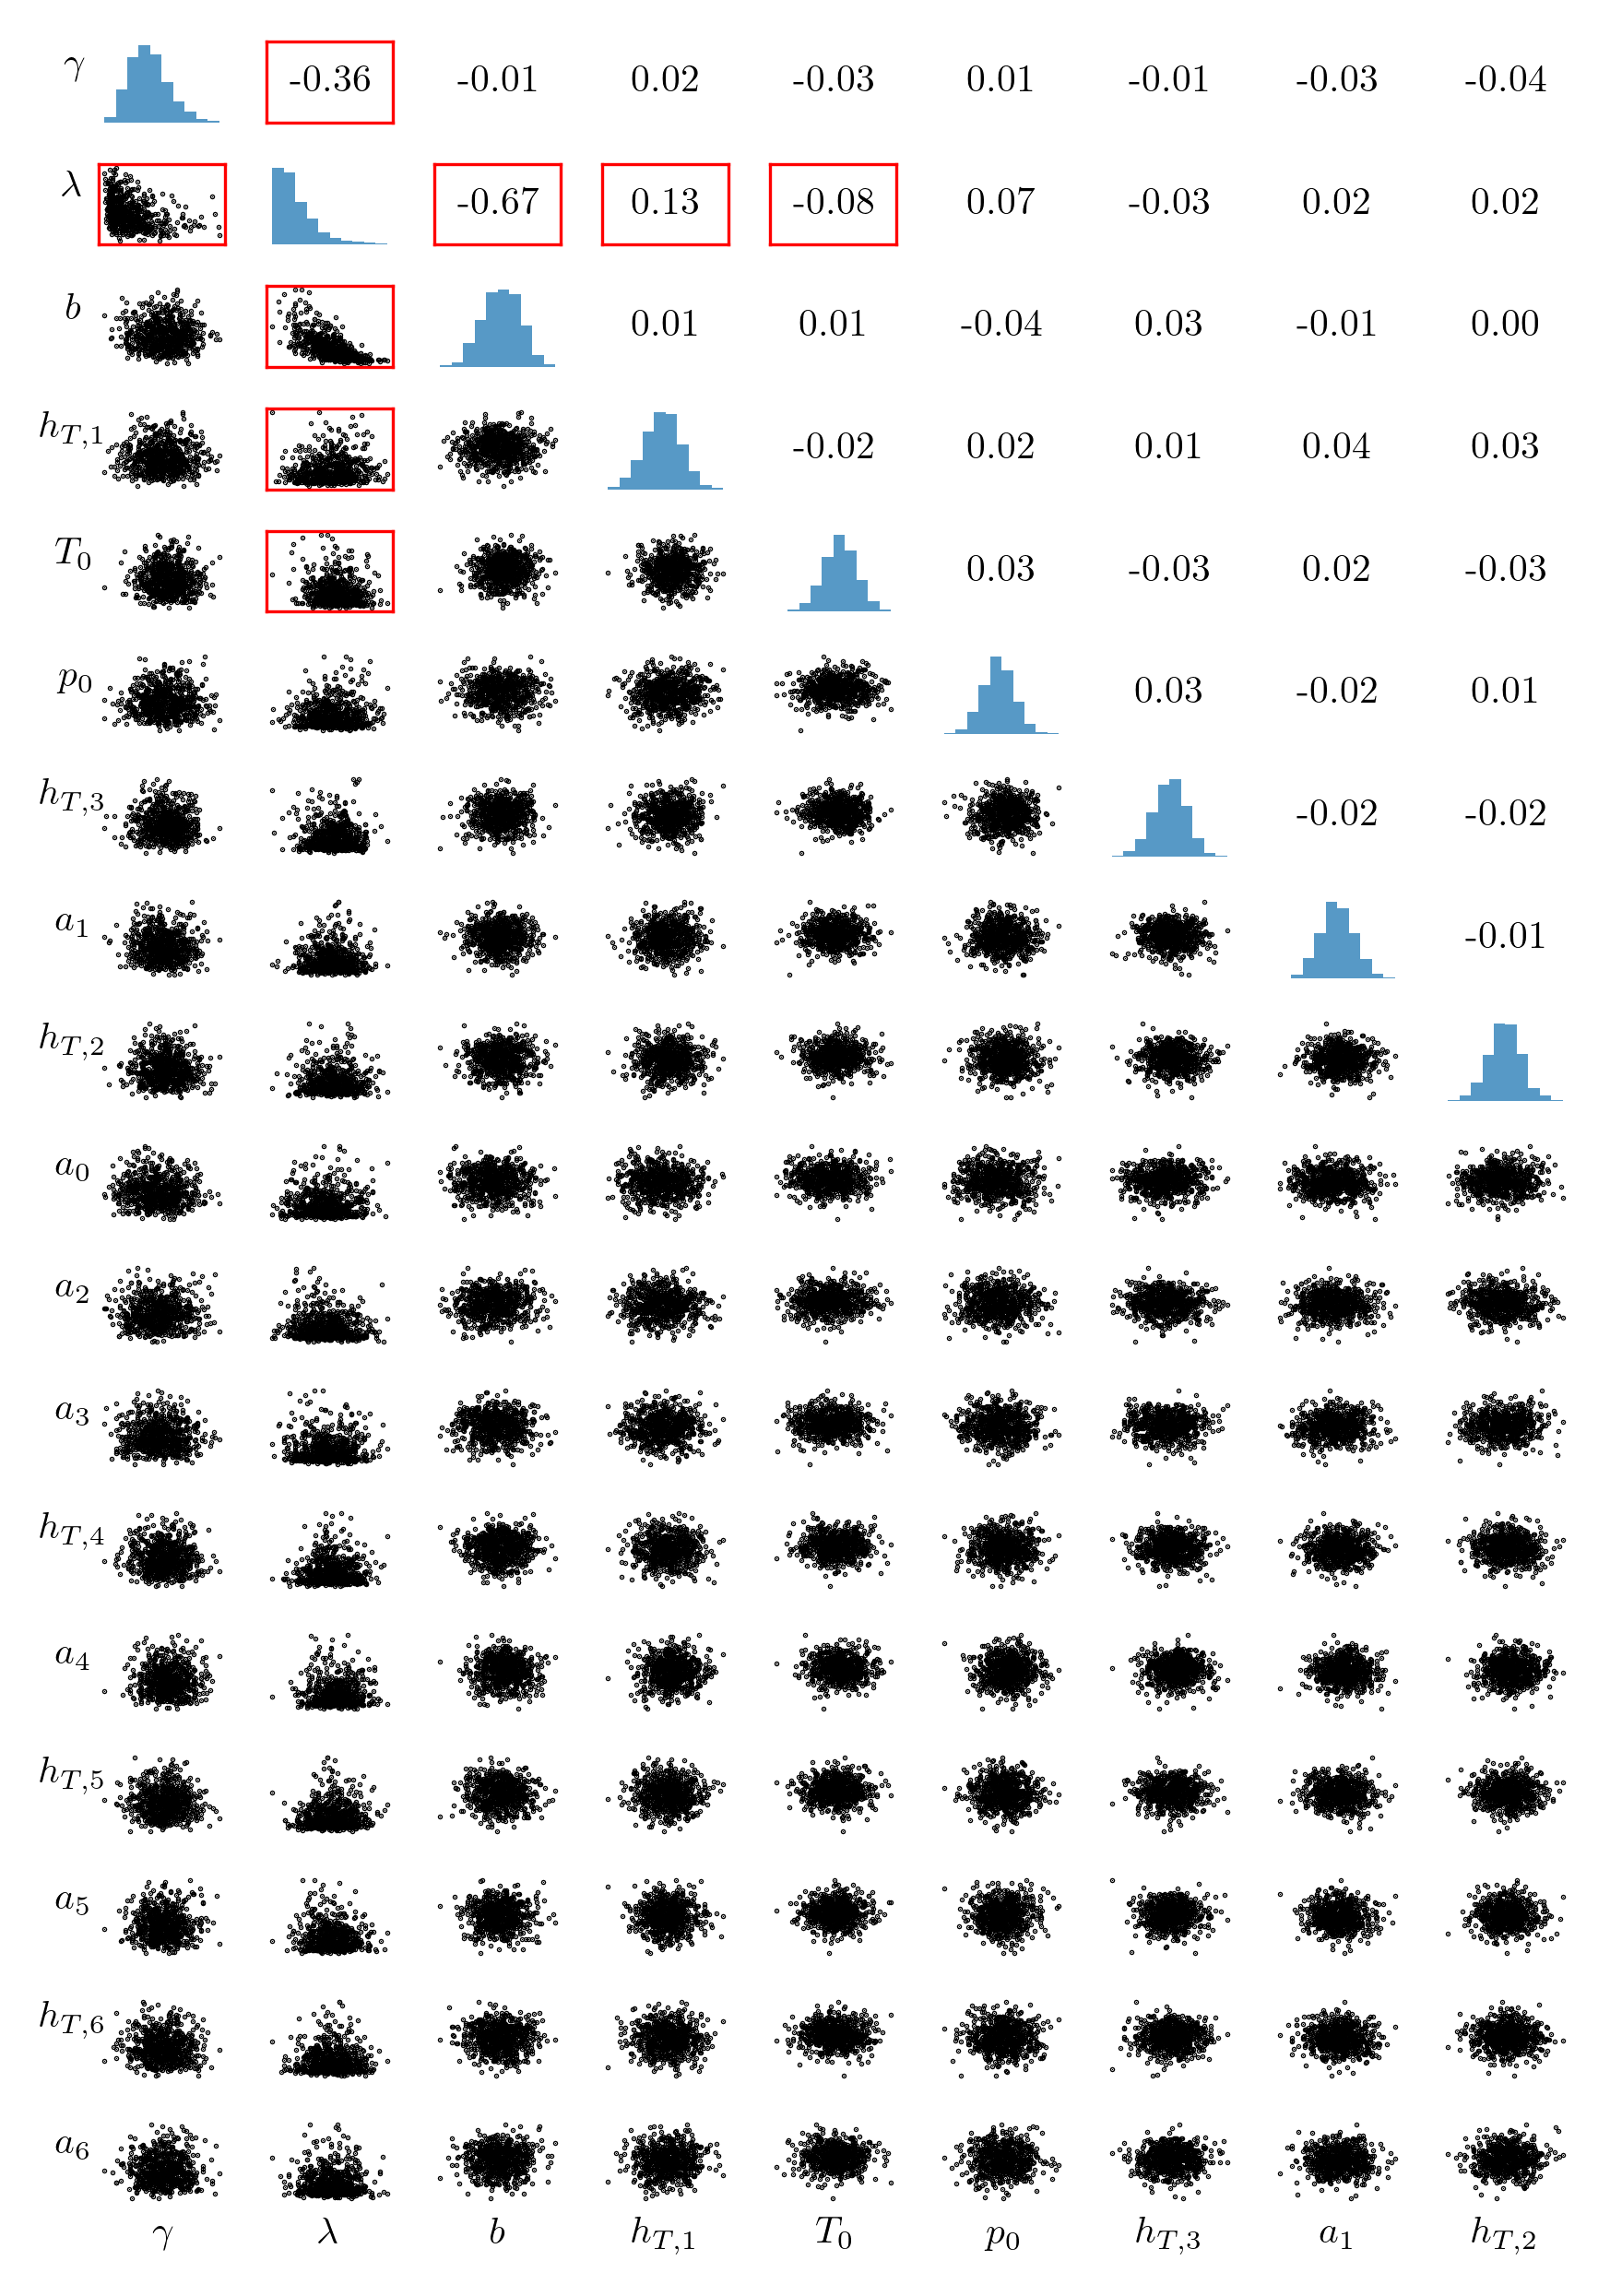
\includegraphics[]{CorrPlot.png}
	\caption[Correlation plot of samples from TT approximation]{Plot of 1000 independent samples from TT approximation of $\sqrt{\pi( \bm{\theta}_{\bm{p}, \bm{T}},\lambda,\gamma  | \bm{y})}$ via SIRT-MH  scheme. We plot the Pearson correlation coefficient ranging from $-1$ to $1$ for each hyper-parameter pair.}
	\label{fig:CorrPlot}
\end{figure}
\begin{figure}% will be the right-side figure
	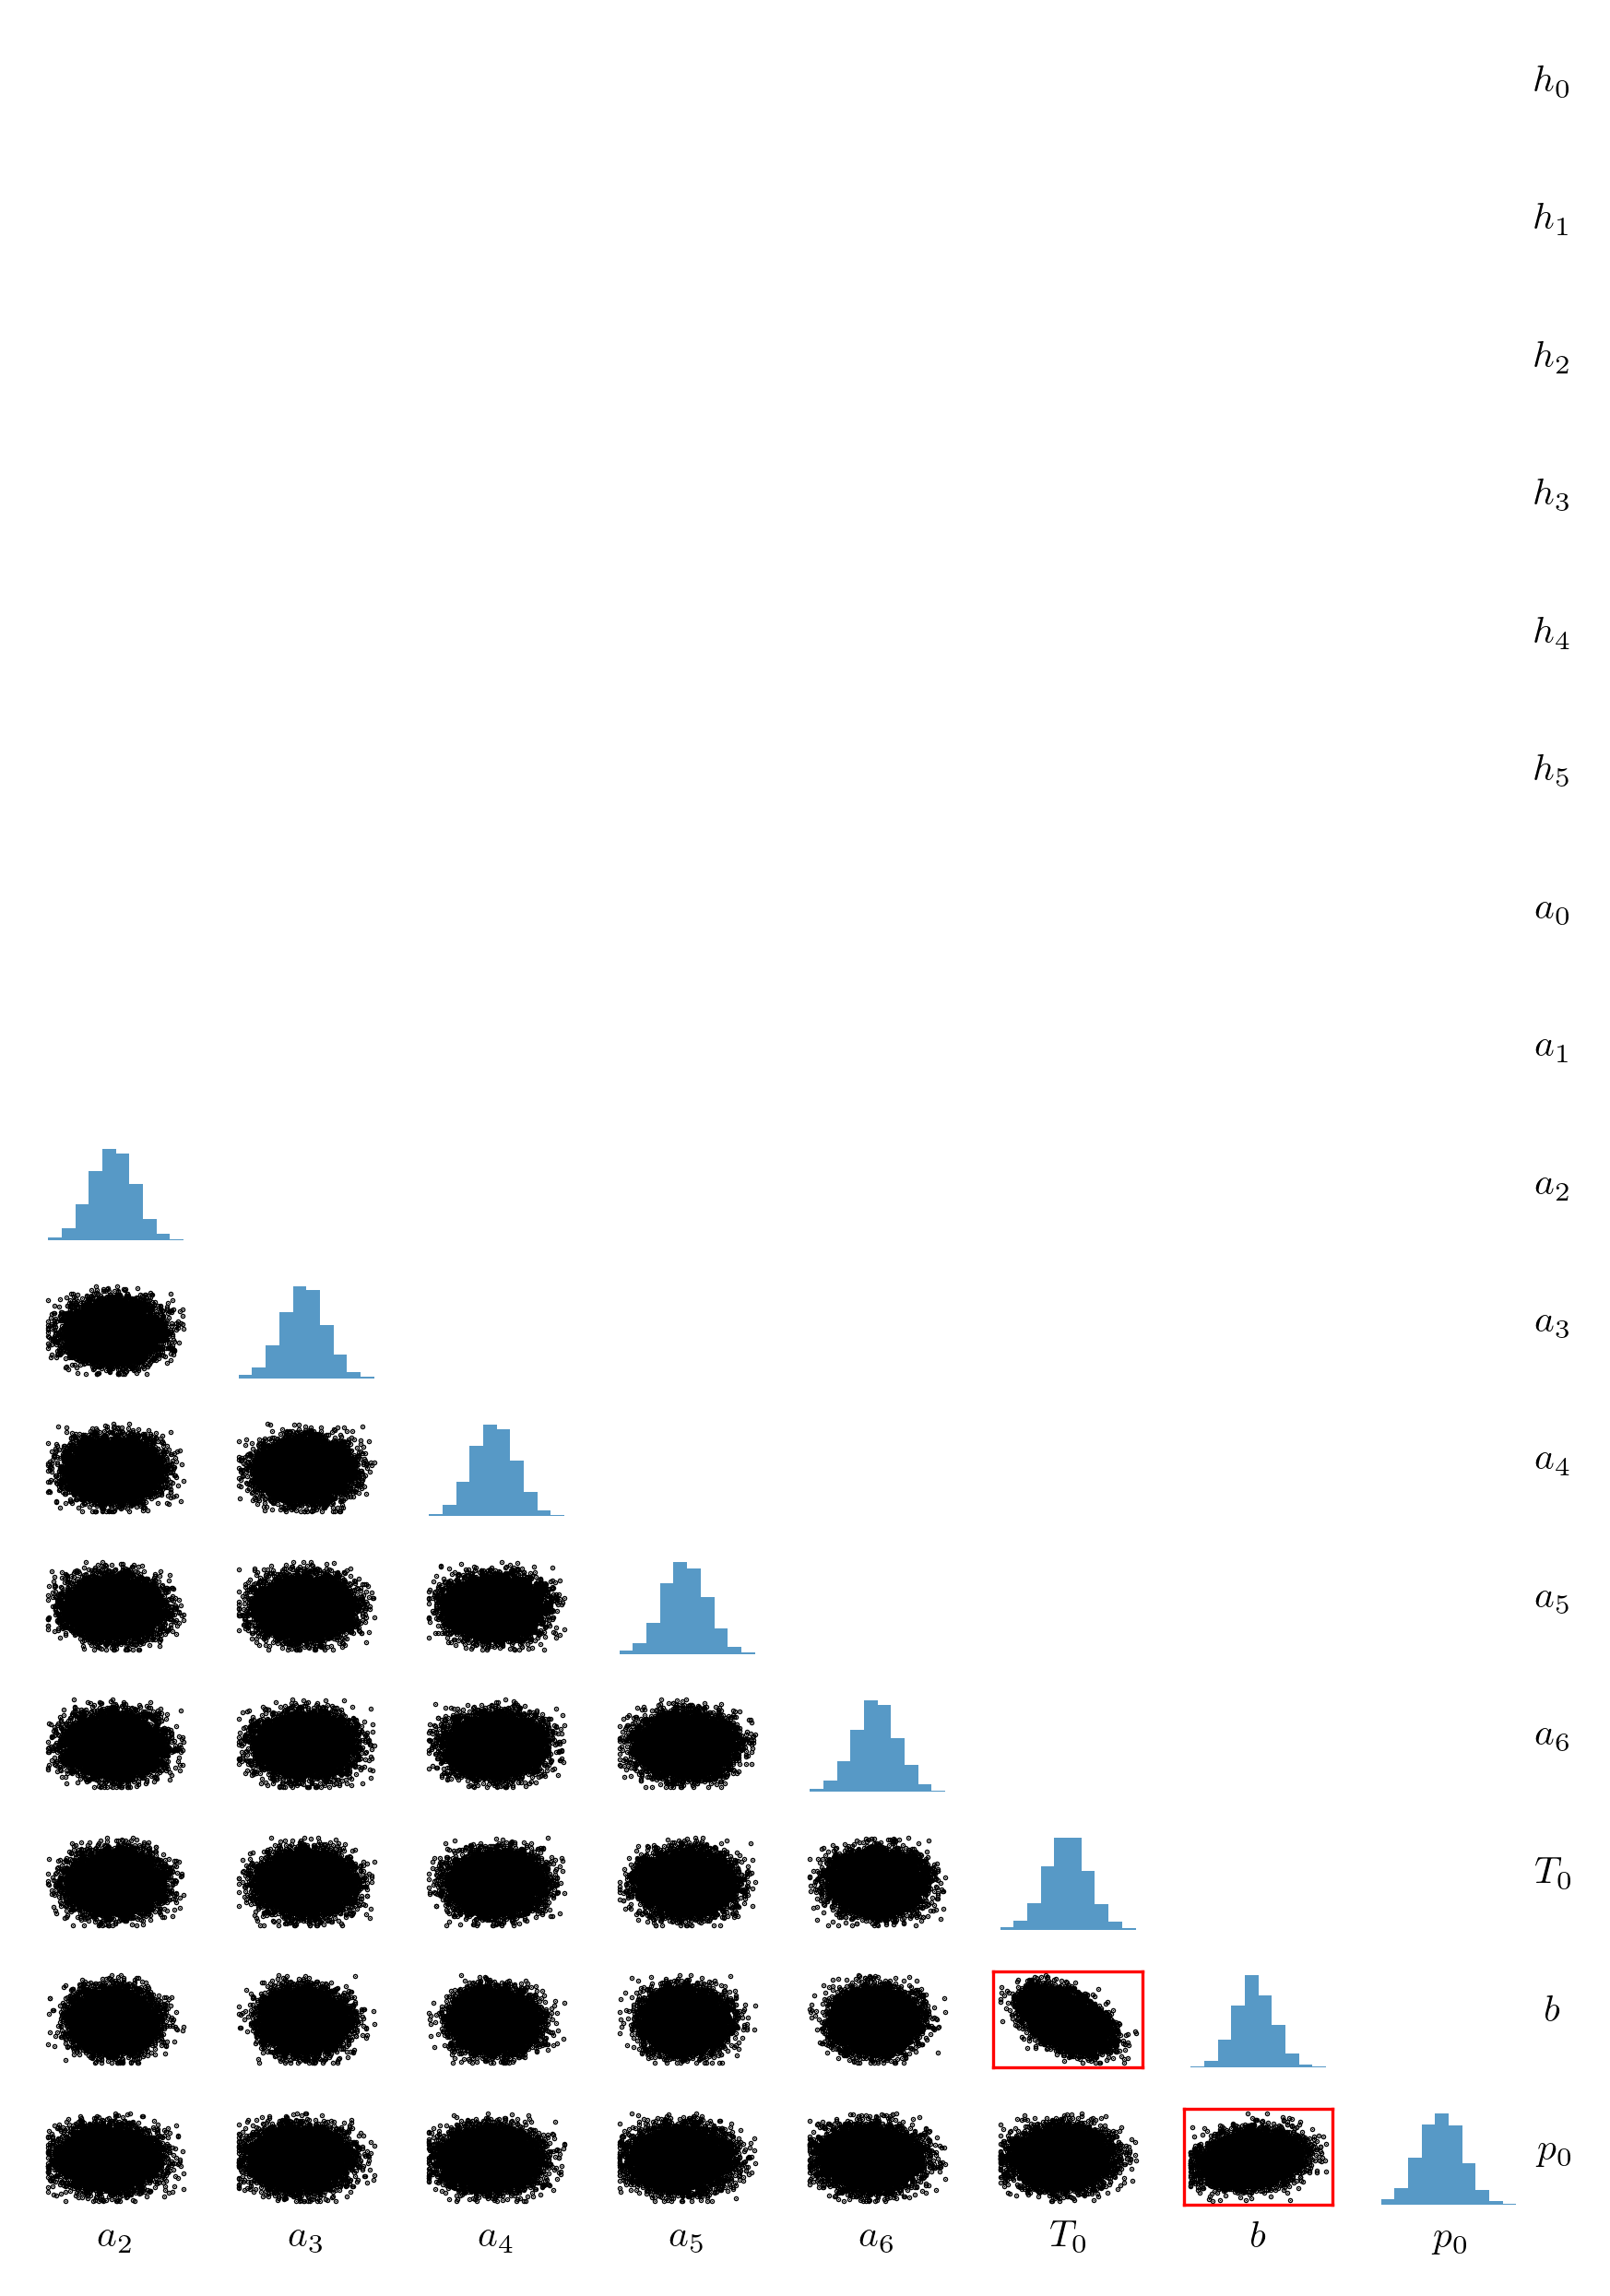
\includegraphics[]{2ndCorrPlot.png}
	\caption*{Correlation plot of samples from TT-approximation of $\sqrt{\pi(p_0,b,T_0,\bm{h_T},\bm{a_T} | \bm{y}, \gamma, \bm{x})}$ via SIRT scheme.}
\end{figure}
\cleardoublepage


\subparagraph{Find optimal rank and grid size}
Next we aim to determine the optimal rank and grid size to accurately approximate the marginal posterior, while decreasing the number of function evaluation.
We set the number of grid points to $n = 150$ and calculate different error measures for deceasing number of ranks to find the optimal number of ranks, where we compare to true marginal posterior function values and $1000$ independent t-walk samples from that distribution.
Then we fix a small but tolerable rank and decrease the number of grid points until sufficient accuracy.

\begin{figure}[ht!]
	\centering% will be the left-side figure
	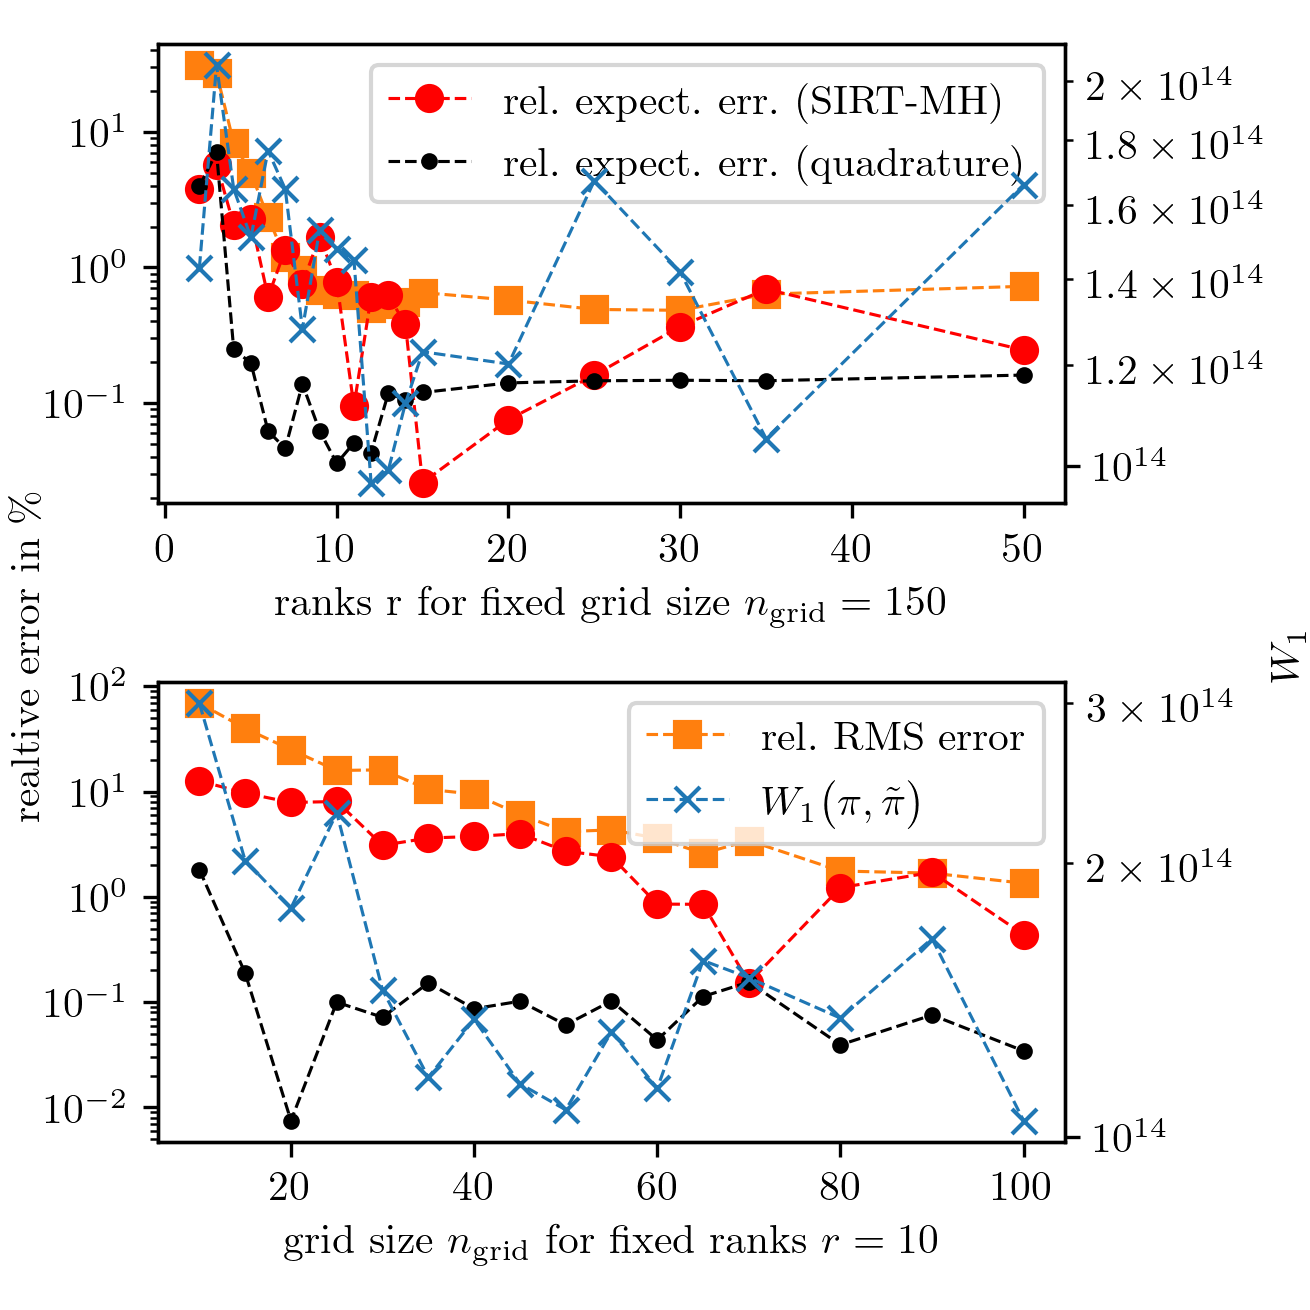
\includegraphics[]{findGridRank.png}
	\caption[Optimal rank and number of grid points for TT approximation.]{Given a TT approximation of $\sqrt{\pi( \lambda,\bm{\theta}_{\bm{p}, \bm{T}},\gamma  | \bm{y}) }$, we calculate the relative RMS error (orange squares) and the 1-Wasserstein distance (blue cross) between approximated values at sample points provided by the SIRT-MH and the true function values. We calculate the relative RMS error between the sample mean provided by the t-walk and mean values for the hyper-parameters calculated by quadrature (black dots), where we use the marginal function from the TT approximation as weights. Additionally, we plot the relative RMS error between the sample-based mean from the SIRT-MH and the t-walk (red circles).}
	\label{fig:FindRankGrid}
\end{figure}
For stable and comparable results, we do five sweeps in \linebreak the~\texttt{tt.cross.rectcross.rect\_cross.cross} python function initialised with a random TT.
Then we draw $1000$ independent samples from the TT approximation of the marginal posterior via the SIRT-MH scheme. 
To calculate the 1-Wasserstein distance, as in Eq.~\ref{eq:applWasser}, between SIRT-MH samples weighted with the TT approximation of marginal posterior and the t-walk samples, weighted by the true marginal posterior values, we use the \texttt{SamplesLoss("sinkhorn", p=1, blur=0.05, scaling=0.8)} function with default settings from the Python package \texttt{geomloss}~\cite{Wassersteinaccess}.
This provides the unbiased Sinkhorn divergence, which converges towards the Wasserstein distance and can be understood as the generalised Quicksort algorithm~\cite{feydy2020OT}.
Here, p = 1 defines the distance measure $\lVert \bm{x} -\tilde{\bm{x}} \rVert_{L^2}$, the blur parameter is an entropic penalty and the scaling parameter specifies the trade-off between speed (scaling $< 0.4$) and accuracy (scaling $>0.9$)~\cite{Wassersteinaccess}.
Additionally, we use the marginal functions of each TT approximation to calculate the means $\bm{\mu}_{\text{TT}} \in \mathbb{R}^{18}$ of each hyper-parameter by weighted expectations.
Then we obtain the relative RMS difference $\lVert\bm{\mu}_{\text{TT}} - \bm{\mu}_{\text{t-walk}} \rVert_{L^2} / \lVert \bm{\mu}_{\text{t-walk}} \rVert_{L^2} $.
Here $\bm{\mu}_{\text{t-walk}}$ denotes the ``true sample-based means'' from the t-walk.
Further, we calculate the relative RMS between the SIRT-MH sample-based mean $\bm{\mu}_{\text{SIRT-MH}}$ and $\bm{\mu}_{\text{t-walk}}$, and the relative RMS error at SIRT-MH samples compared to ground truth function values (Eq.~\ref{eq:RMSTT}).

We plot all of these measures in Fig.~\ref{fig:FindRankGrid}, where we observe that a rank $r = 10$ is sufficient because the error measures are relatively stable for $r\geq10$.
Then we decrease the grid size and decide that for $n \geq 20$ the relative differences of sample-based means to $\bm{\mu}_{\text{t-walk}}$ (red circles in Fig.~\ref{fig:FindRankGrid}) and the RMS error at the SIRT-MH samples (orange squares in Fig.~\ref{fig:FindRankGrid}) around $ 20\%$ is good enough.
We relate a more accurate interpolation in between grid points to decreasing sample-based relative errors for an increasing number of grid points, since the chosen linear interpolation (see Eq.~\ref{eq:LinPol}) is a rather rudimentary choice.
The quadrature-based relative expectation error (black dots in Fig.~\ref{fig:FindRankGrid}) is almost constant for ranks $\geq 7$ and grid sizes $\geq15$.
Since the hyper-parameters have different length scales, we are only interested in the trend of the 1-Wasserstein distance (blue crosses in Fig.~\ref{fig:FindRankGrid}).
The 1-Wasserstein distance is quite fluctuant but decreases with increasing ranks and stays within a similar range for decreasing grid size.


\begin{figure}[ht!]
	\centering
	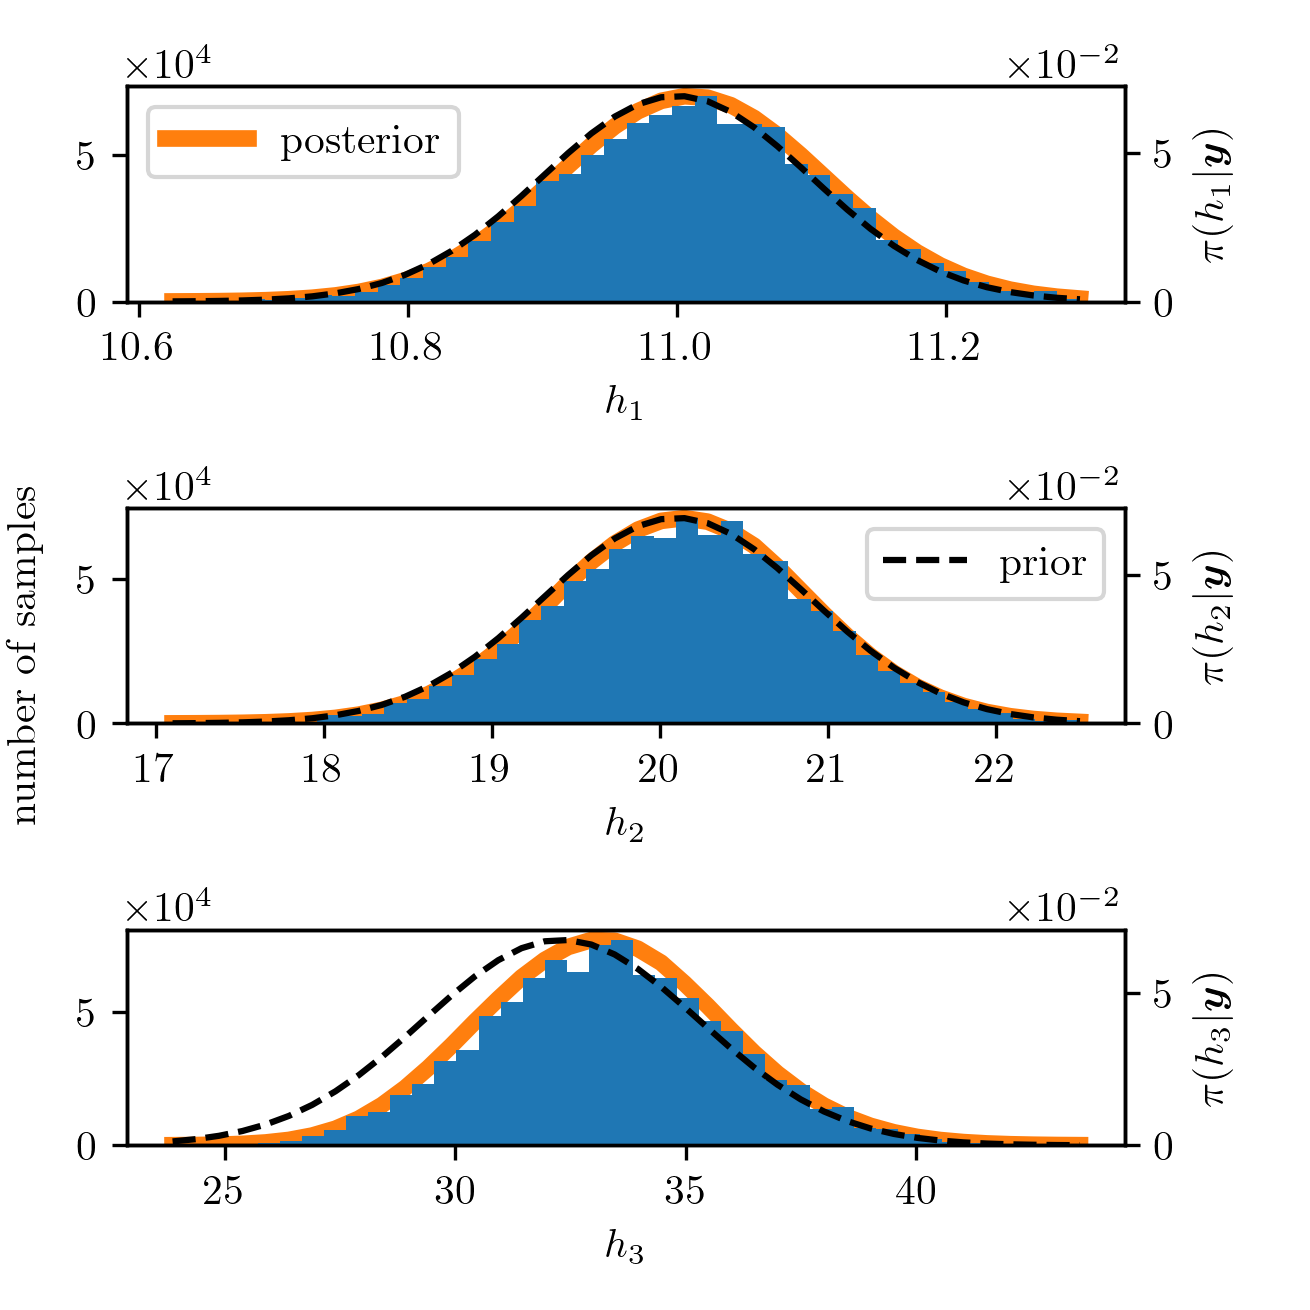
\includegraphics{PHdPTPost0.png}
	\caption[Histograms and TT approximation of posterior distribution as well as hyper-prior distribution.]{TT approximation of the marginal posterior in orange and the samples as a histogram as well as the prior distribution with a dotted line.}
	\label{fig:PostHistTT0}
\end{figure}
\begin{figure}[ht!]
	\centering
	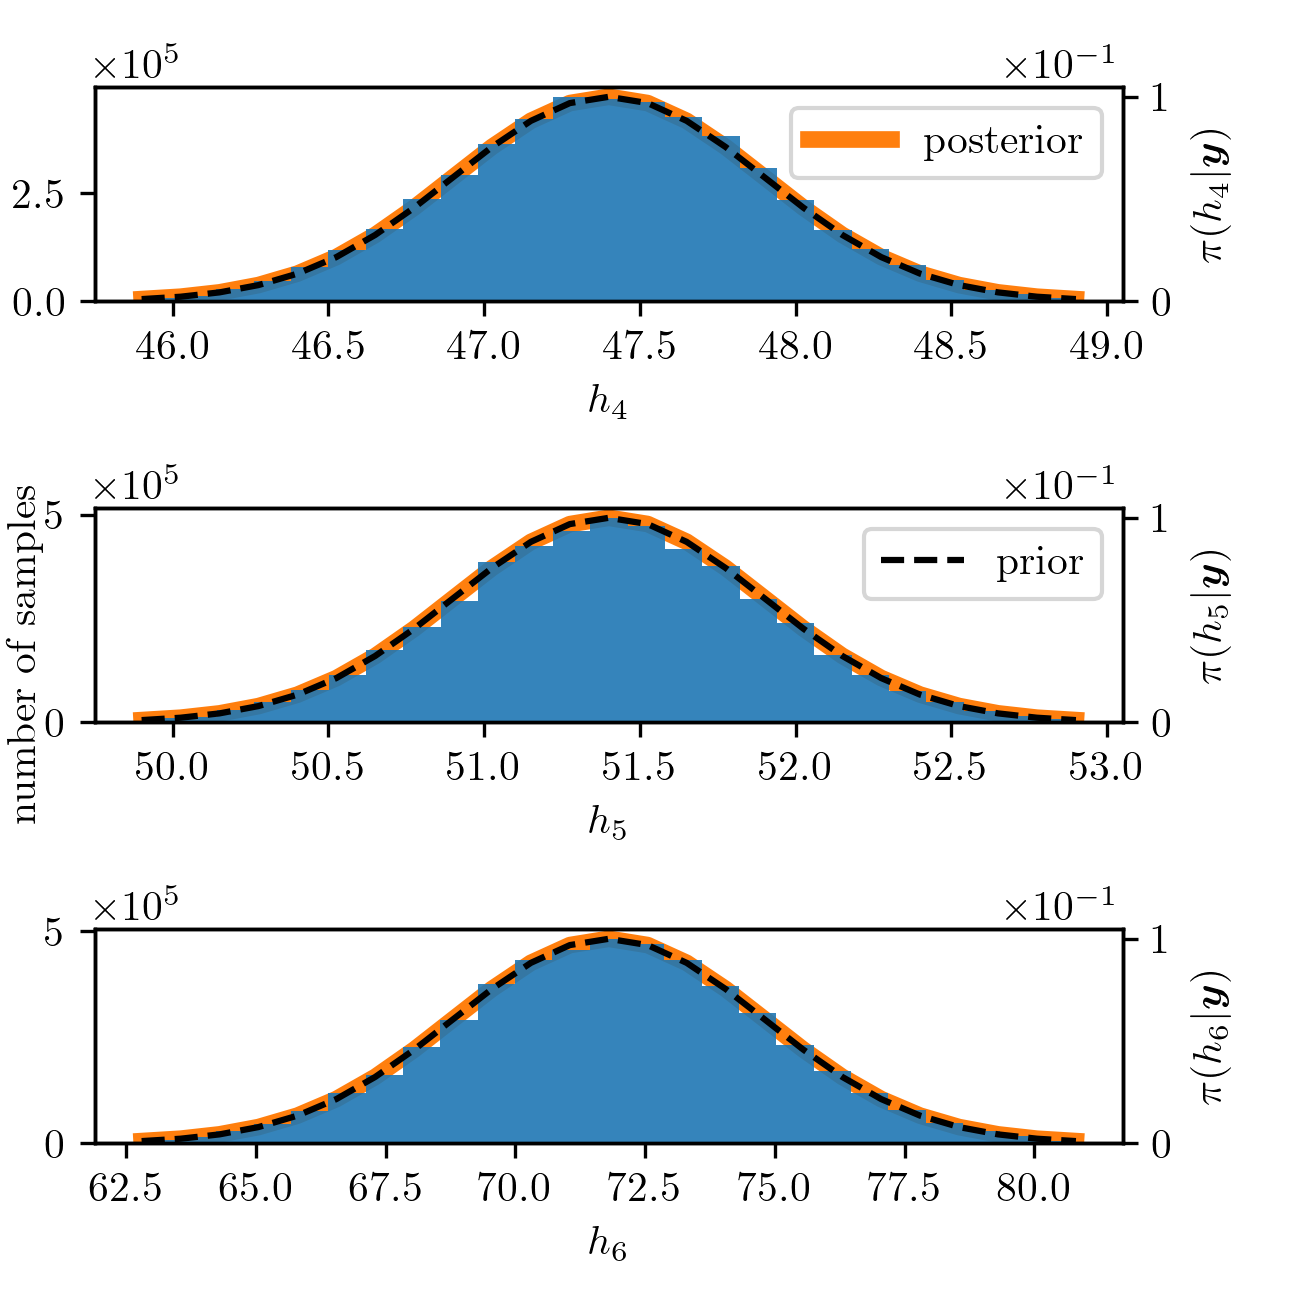
\includegraphics{PHdPTPost1.png}
	\caption[Histograms and TT approximation of posterior distribution as well as hyper-prior distribution.]{TT approximation of the marginal posterior in orange and the samples as a histogram as well as the prior distribution with a dotted line.}
	\label{fig:PostHistTT1}
\end{figure}
\begin{figure}[ht!]
	\centering
	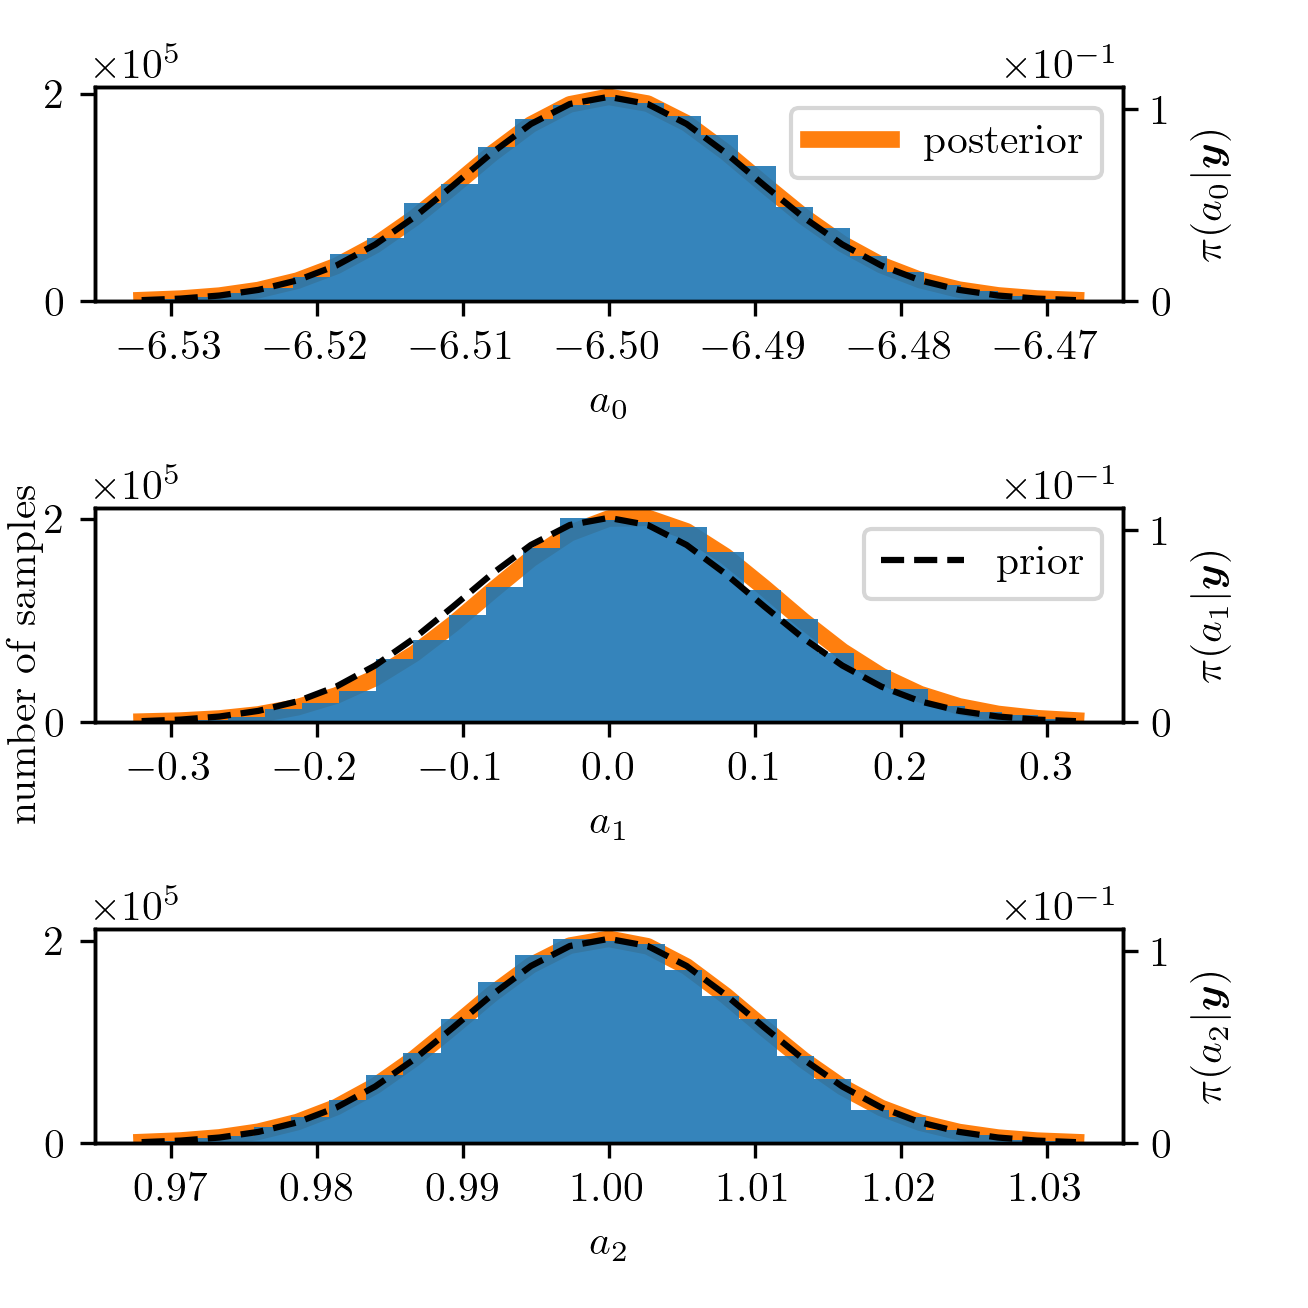
\includegraphics{PHdPTPost2.png}
	\caption[Histograms and TT approximation of posterior distribution as well as hyper-prior distribution.]{TT approximation of the marginal posterior in orange and the samples as a histogram as well as the prior distribution with a dotted line.}
	\label{fig:PostHistTT2}
\end{figure}
\begin{figure}[ht!]
	\centering
	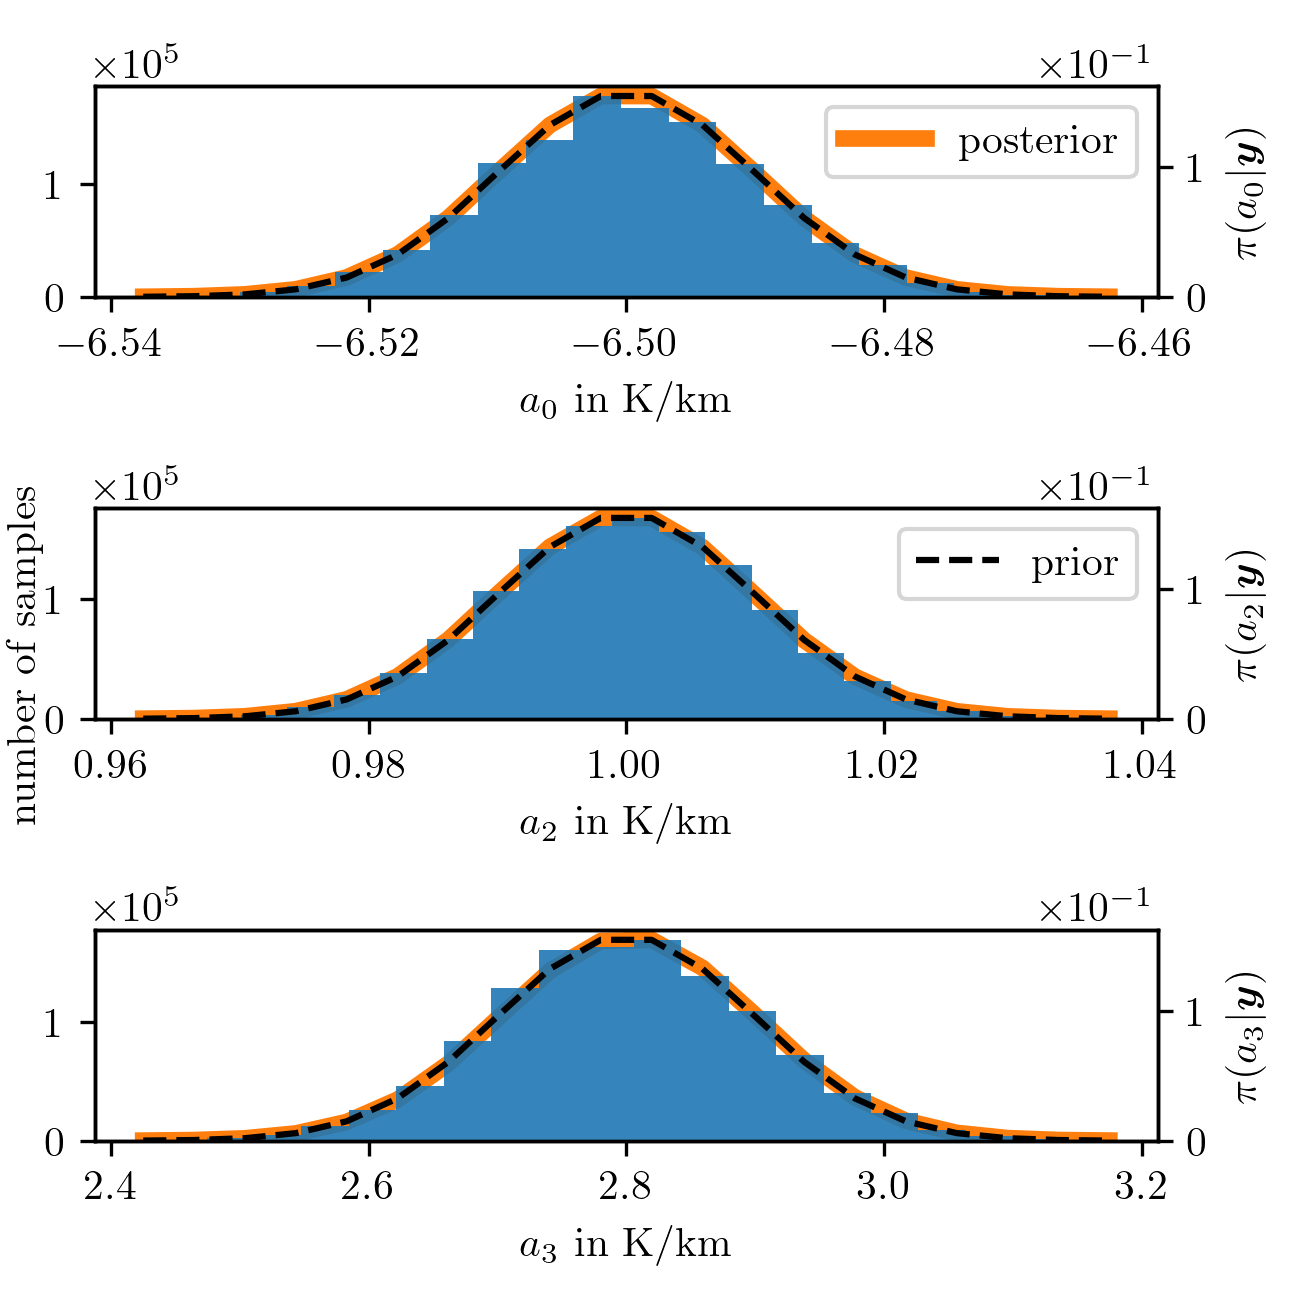
\includegraphics{PHdPTPost3.png}
	\caption[Histograms and TT approximation of posterior distribution as well as hyper-prior distribution.]{TT approximation of the marginal posterior in orange and the samples as a histogram as well as the prior distribution with a dotted line.}
	\label{fig:PostHistTT3}
\end{figure}
\begin{figure}[ht!]
	\centering
	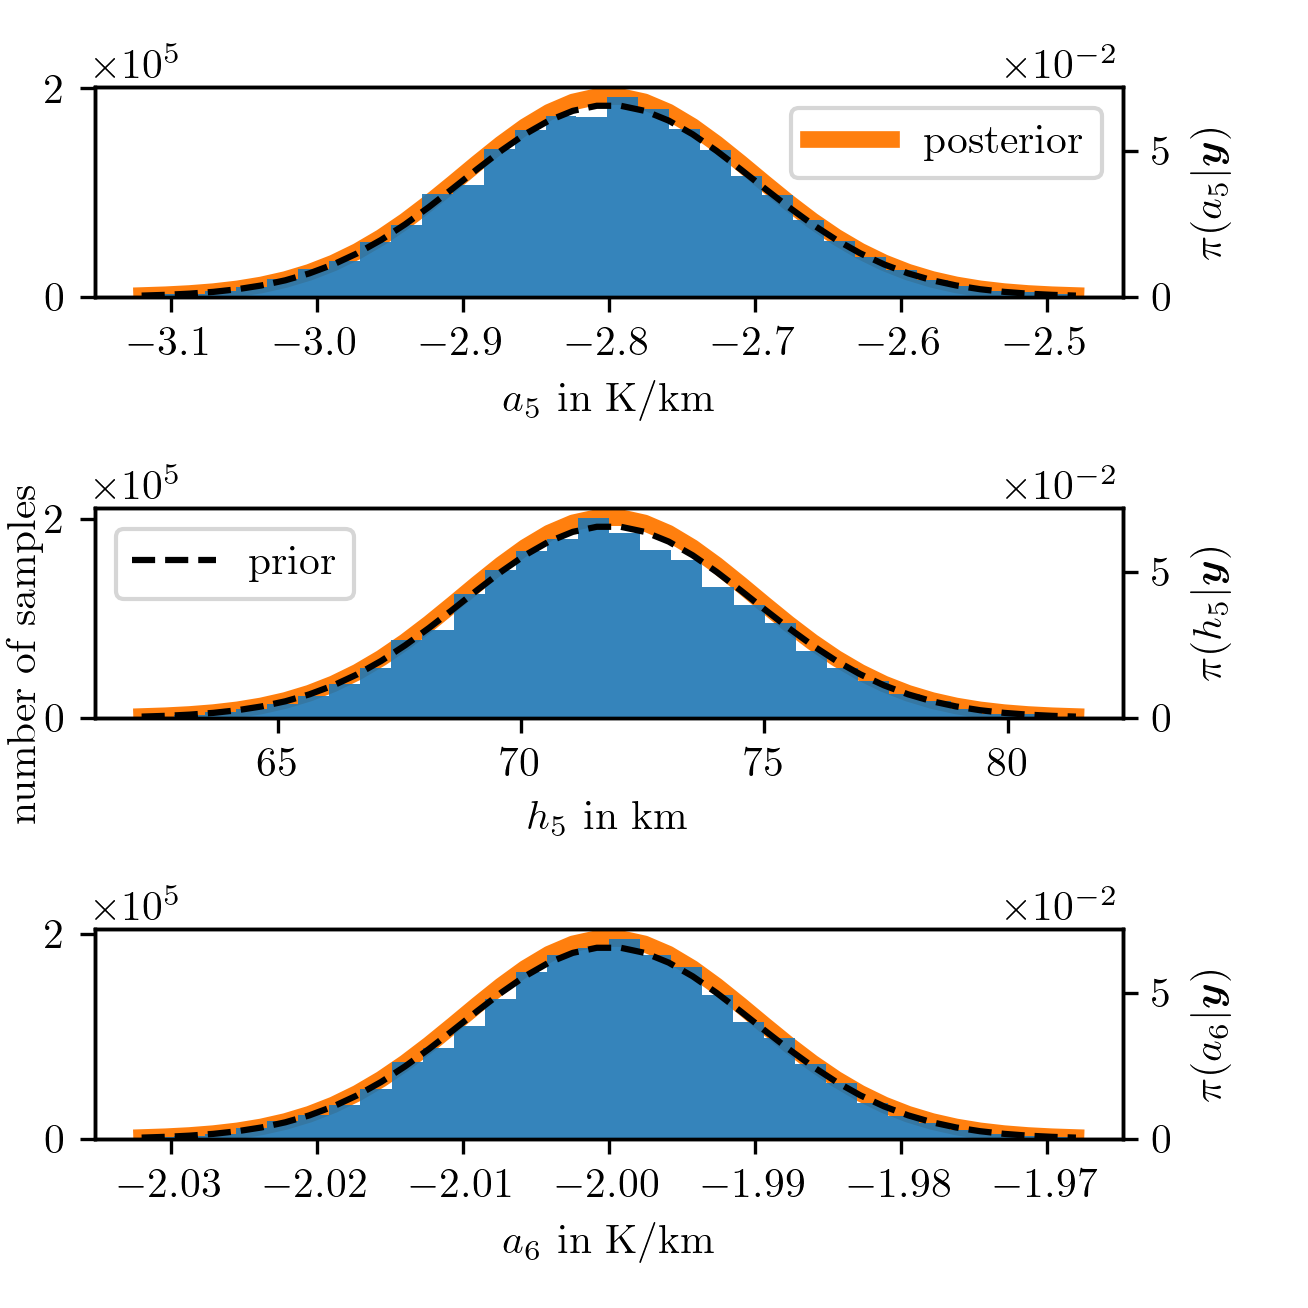
\includegraphics{PHdPTPost4.png}
	\caption[Histograms and TT approximation of posterior distribution as well as hyper-prior distribution.]{TT approximation of the marginal posterior in orange and the samples as a histogram as well as the prior distribution with a dotted line.}
	\label{fig:PostHistTT4}
\end{figure}
\begin{figure}[ht!]
	\centering
	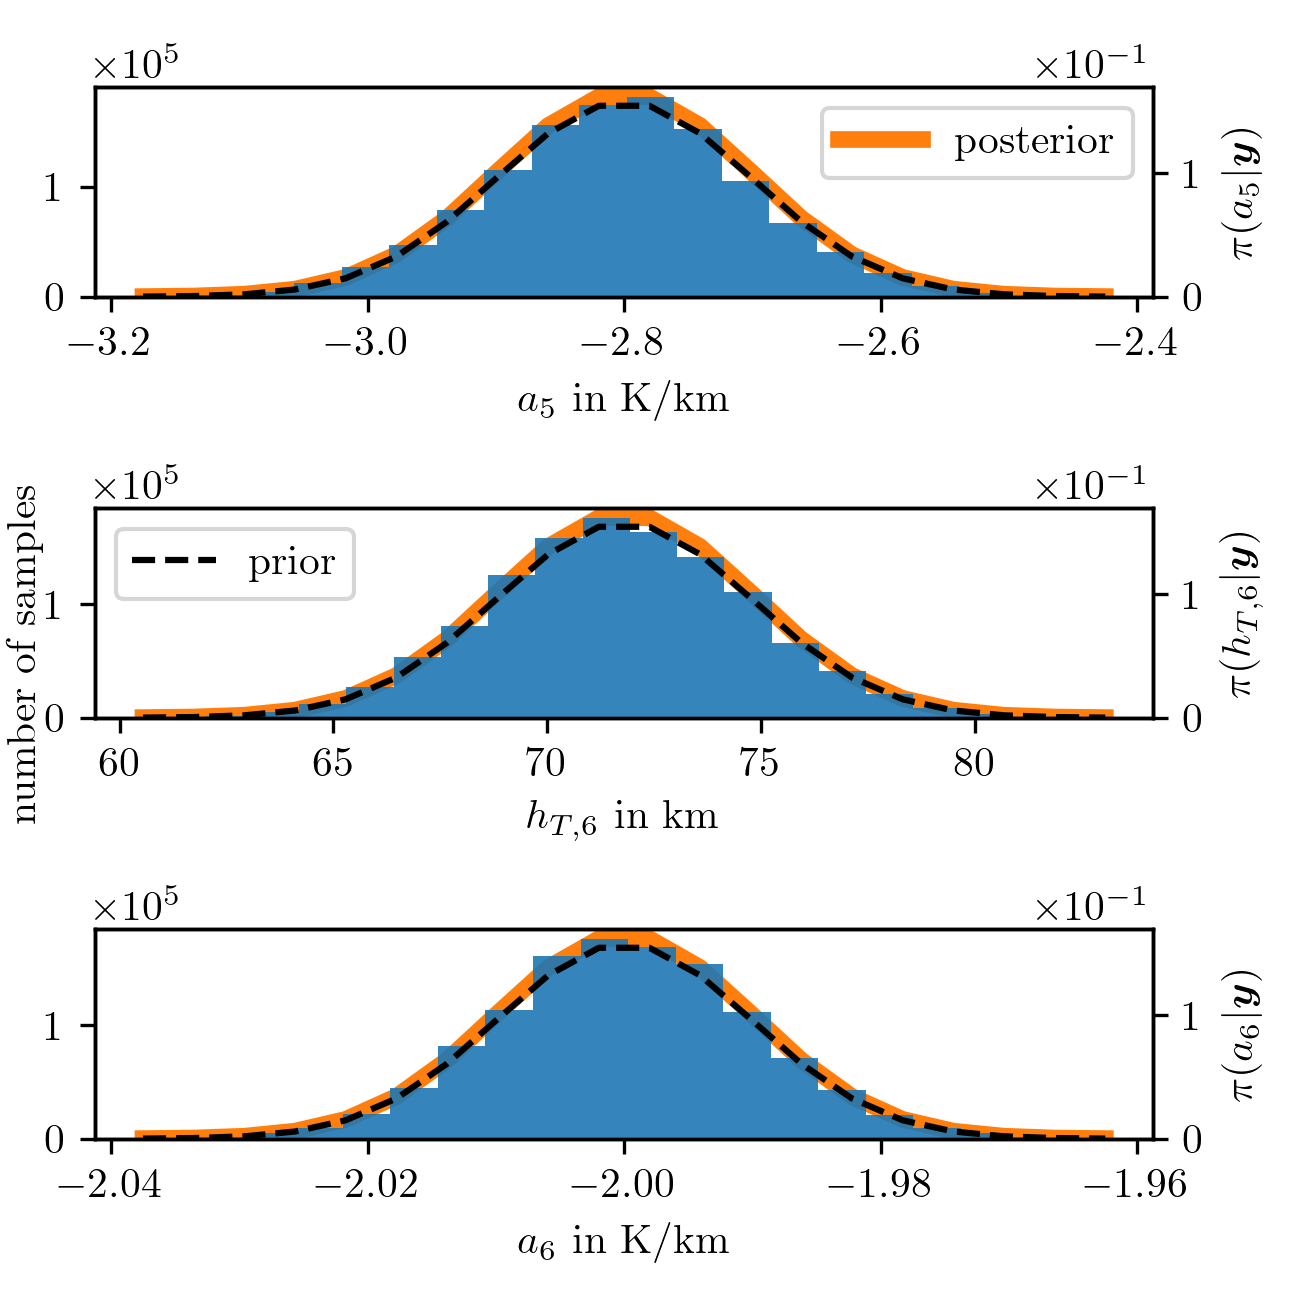
\includegraphics{PHdPTPost5.png}
	\caption[Histograms and TT approximation of posterior distribution as well as hyper-prior distribution.]{TT approximation of the marginal posterior in orange and the samples as a histogram as well as the prior distribution with a dotted line.}
	\label{fig:PostHistTT5}
\end{figure}

Further, we decrease the number of functions evaluations and define ranks \linebreak$r = [ 1,  10,  10, 10, 10, 10, 5, 5, 5, 5, 5, 3, 2, 2, 2, 2, 2, 2, 1]$ harvesting the correlation structure of $\pi(\bm{\theta}_{\bm{p}, \bm{T}},\lambda,\gamma  | \bm{y})$ even more.
We do one sweep in \linebreak the~\texttt{tt.cross.rectcross.rect\_cross.cross}, reducing the computation time to $\approx 7$s and the number of function evaluations to 24120, where we initialise at a previously calculated approximation.
We report an average IACT (provided by~\cite{wolff2004monte, drikHesse}) of $\approx 1.2 \pm 0.2$ for the samples drawn via the SIRT-MH scheme, which means that we need two function evaluations per independent sample, once the TT approximation is available.
\textcolor{red}{To draw 1000 independent samples, including generating a TT approximation, takes $\approx30$s, and we report a relative RMS error of $\approx 25 \%$ evaluated over those 1000 independent samples.
Additionally, we report a relative RMS error of $\leq 1\%$ on 1000 randomly chosen grid points, indicating that the linear interpolation causes most of the approximation error.}
We plot the marginals for each hyper-parameter in Fig.~\ref{fig:PostHistTT0} to Fig.~\ref{fig:PostHistTT5} and samples in Fig.~\ref{fig:CorrPlot}.
We observe that, besides $\lambda$ and $\gamma$, only the marginal posterior of the $b$ hyper-parameter is seriously affected by the data and has significantly changed compared to the hyper-prior distribution.
\clearpage

\subsubsection{Full conditional posterior distribution}
We use the RTO method (see Sec.~\ref{subsec:RTO}) to obtain ozone samples from the full conditional posterior and sample hyper-parameter samples directly from the marginal posterior to compute posterior temperature and pressure profiles according to their respective function (see Eq.~\ref{eq:tempFunc} and Eq.~\ref{eq:pressFunc}). 
We plot posterior profiles of ozone in Fig.~\ref{fig:O3Post}, temperature in Fig.~\ref{fig:TempPost} and pressure in Fig.~\ref{fig:PressPost}.
\begin{figure}[ht!]
	\centering
	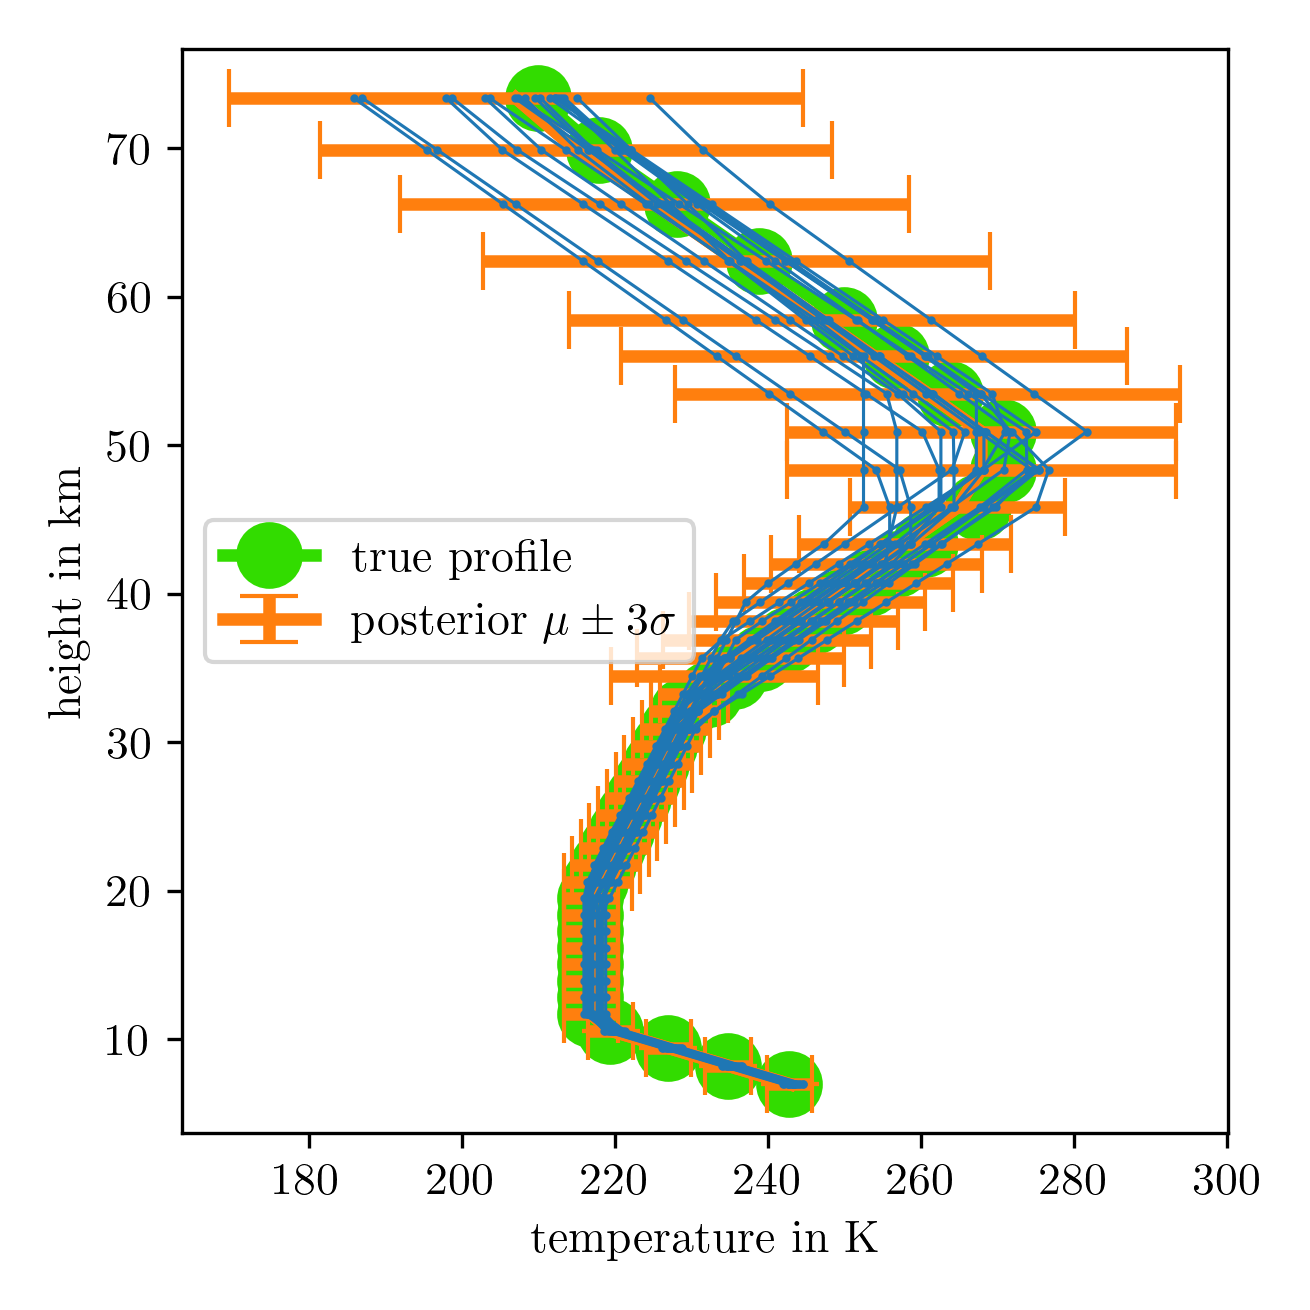
\includegraphics{TempPostMeanSigm.png} 
	\caption[Temperature posterior samples.]{According to the hyper-parameter samples from the marginal posterior distribution (see Fig.~\ref{fig:PostHistTT1} to Fig.~\ref{fig:PostHistTT5}) we plot the corresponding posterior temperature profile as given by Eq.~\ref{eq:tempFunc}. }
	\label{fig:TempPost}
\end{figure}

\begin{figure}[ht!]
	\centering
	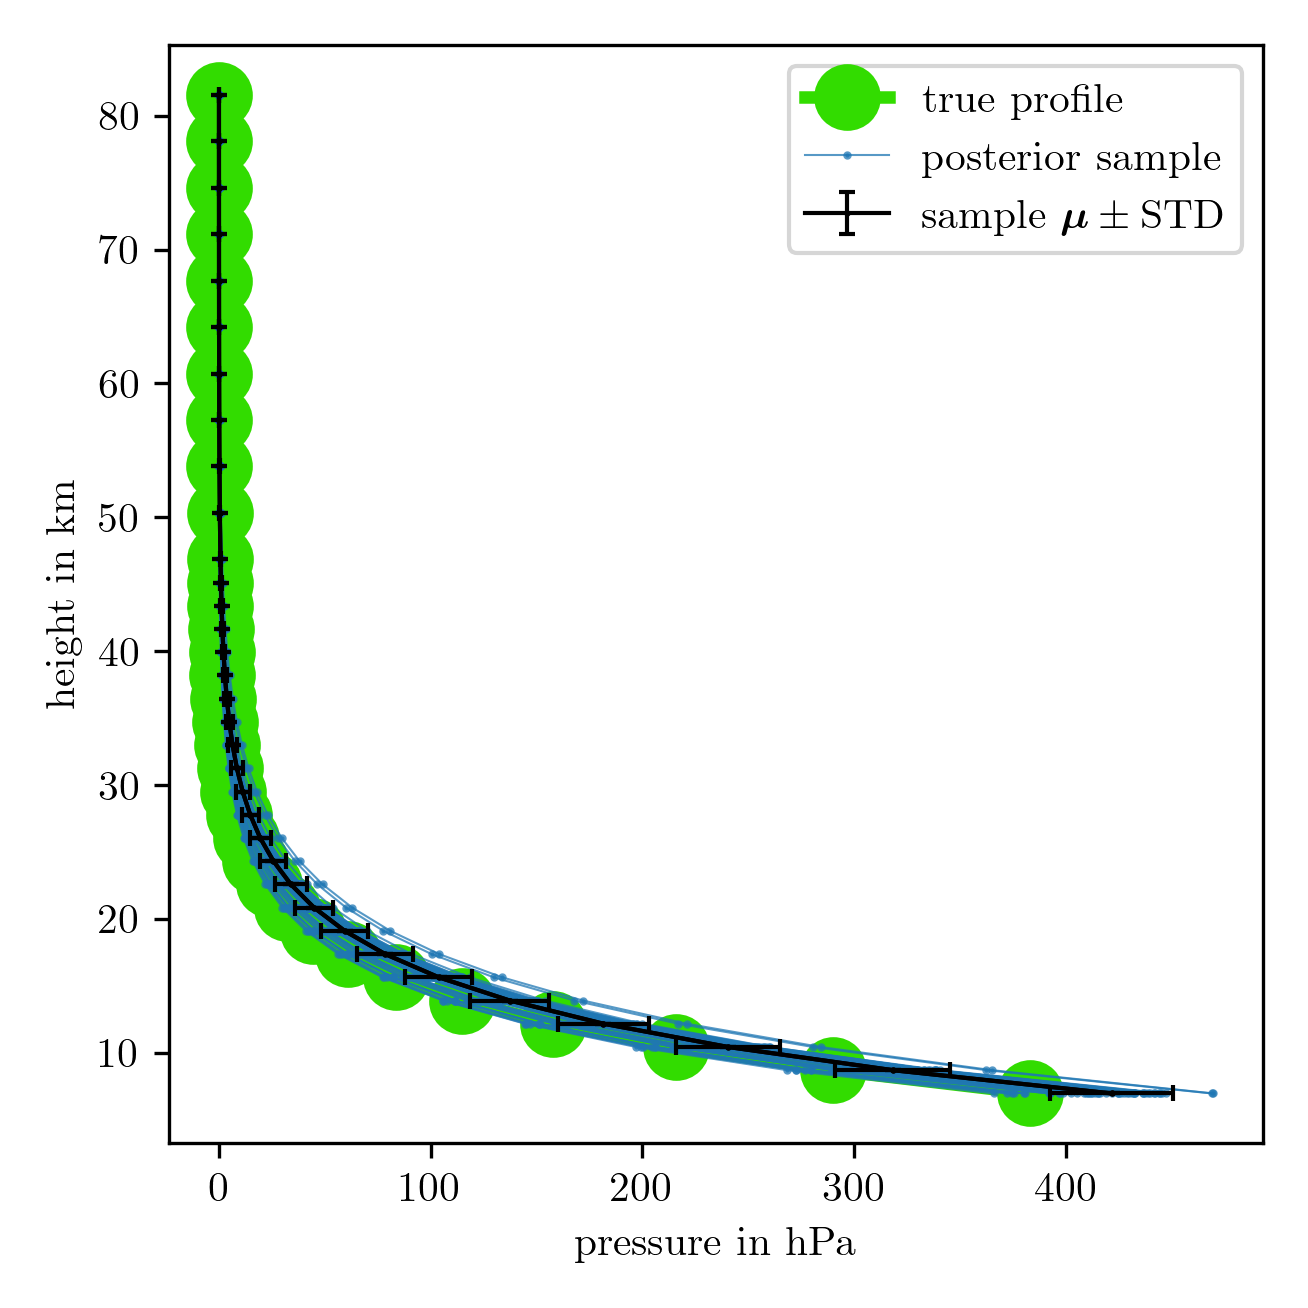
\includegraphics{PressPostMeanSigm.png}
	\caption[Pressure posterior samples.]{According to the hyper-parameter samples from the marginal posterior distribution (see Fig.~\ref{fig:PostHistTT0} and Fig.~\ref{fig:PostHistTT1}) we plot the corresponding posterior pressure profile as given by Eq.~\ref{eq:pressFunc}.}
	\label{fig:PressPost}
\end{figure}

\begin{figure}[ht!]
	\centering
	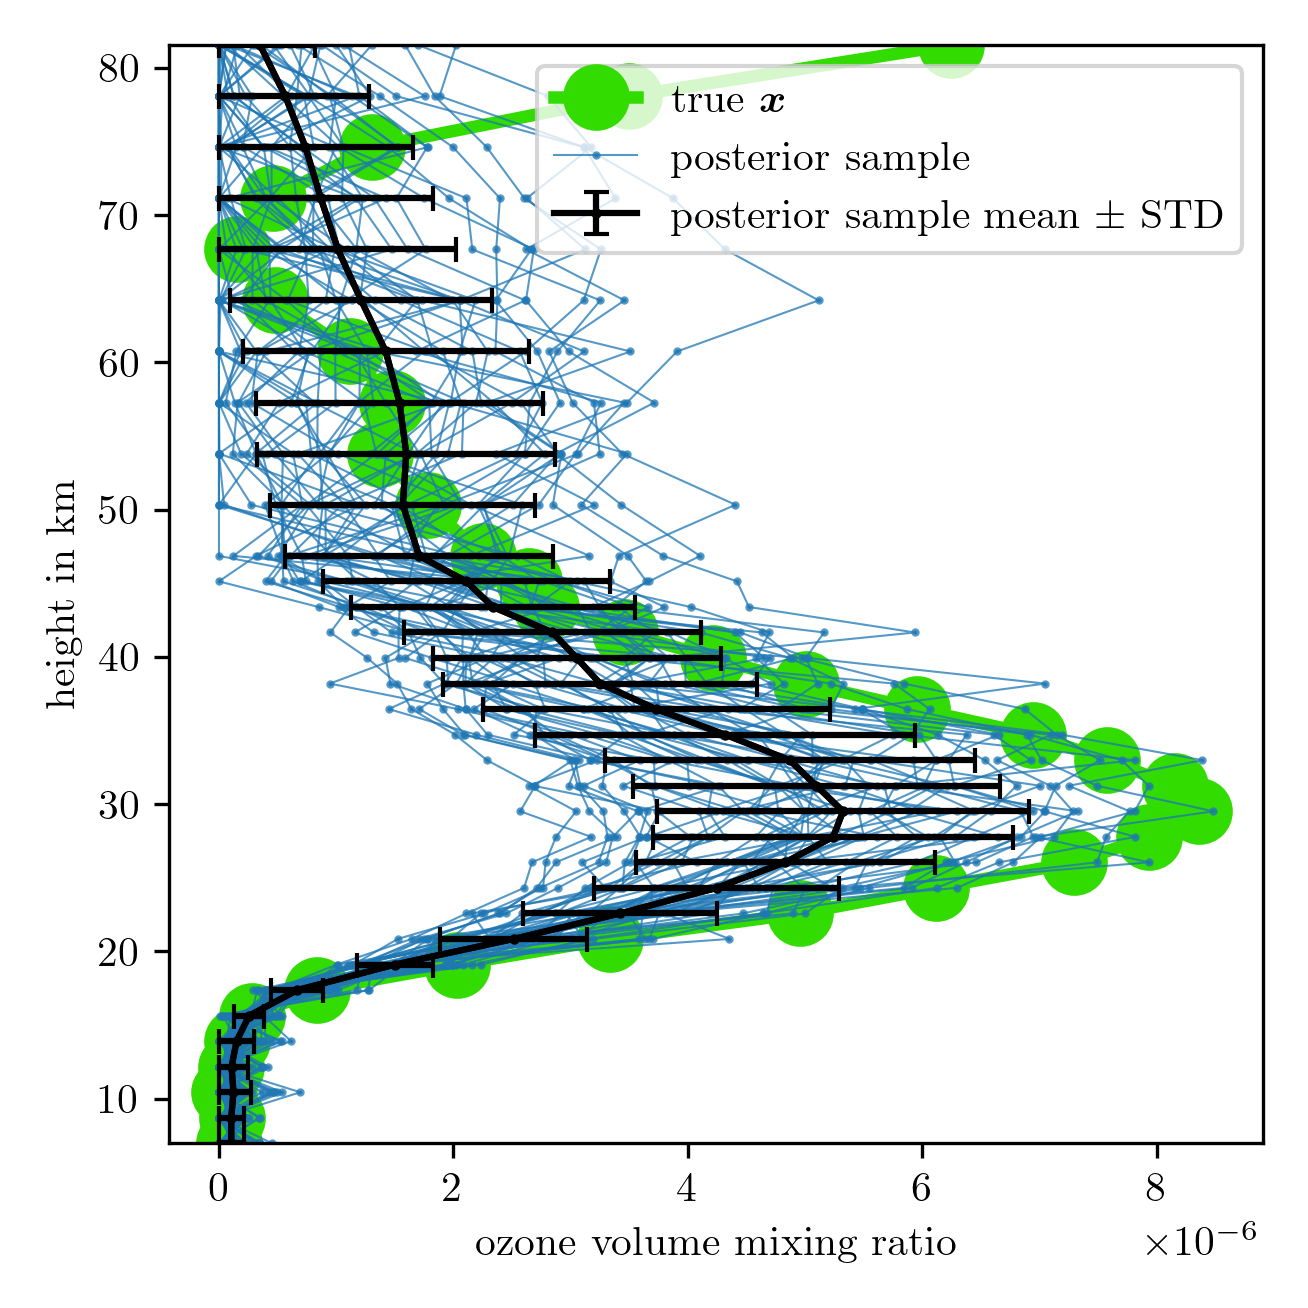
\includegraphics{FullO3Res.png}
	\caption[Pressure posterior samples.]{According to the hyper-parameter samples from the marginal posterior distribution (see Fig.~\ref{fig:PostHistTT0}) we plot the corresponding ozone sample from the full conditional posterior using the RTO method.}
	\label{fig:O3Post}
\end{figure}

We observe that pressure and ozone are highly correlated.
Since the hyper-parameter $b$ is smaller than its ground truth value, the posterior pressure profile does not exponentially decrease as strongly as the ground truth pressure (see Fig.~\ref{fig:PostHistTT0}).
This results in posterior pressure values which are slightly larger than the ground truth, and in an average posterior ozone profile with much smaller peak values compared to the ground truth.
Additionally, the individual posterior samples are more prior-dominated through larger $\lambda$ values (see Fig.\ref{fig:PostHistTT0}) and hence slightly smoother.
Again, we are not able to recover the second peak at high altitudes.
The posterior temperature profiles look (as expected) similar to the prior temperature profiles.
\clearpage




%When approximating the marginal posterior the maximum relative propagation error $\underset{\lambda , \gamma}{\text{arg max}\,}|\tilde{\pi}(\lambda,\gamma|\bm{y}) - \pi(\lambda,\gamma|\bm{y}) |/ |\pi(\lambda,\gamma|\bm{y})|$ is approximately $100\%$ at $\gamma_{\text{max}}$ and $\lambda_{\text{max}}$, which are the maximum values of the $\lambda$ and $\gamma$ samples and lay in regions with very low probability.
%We consider this error negligible because the absolute error at $\gamma_{\text{max}}$ and $\lambda_{\text{max}}$ is smaller than $10^{-24} \approx 0$.
%Note that one can reduce the maximum errors when approximation $f(\lambda)$ at the mean of $\pi(\lambda,\gamma|\bm{y})$ instead of the modes since $\pi(\lambda | \bm{y})$ is skewed, but we don't see noticeable differences in the conditional posterior $\pi(\bm{x}|\lambda,\gamma,\bm{y})$ when doing so.
%We consider these errors as tolerable.
%$\lVert \pi(\bm{x}_{MH}) - \tilde{\pi}(\bm{x}_{MH}) \rVert / \lVert \pi(\bm{x}_{MH}) \rVert$
%$\lVert \mathbb{E}\big[ \bm{x} \big]  -  \mathbb{E} \big[ \tilde{\bm{x}} \big] \rVert_{L^2}$
%$\lVert \mathbb{E}  \big[\bm{x}\big] -  \mathbb{E} \big[ \bm{x}_{MH}\big]  \rVert_{L^2}$
%When we calculate the mean and covariance matrix of the full conditional $\pi(\bm{x}|\bm{y})$ we have to bin up the samples of the marginal posterior $\pi(\gamma, \delta |\bm{y})$ or use a TT approximation on a predefined grid with a certain number of grid points, we like to give an estimate for this error as well.
%In doing we bin up samples and use the height $\tilde{\pi}(\bm{\theta}^{(k)}_d)$ for a bin $k = 1, \dots, \text{N}_b$ to calculate the mean $\tilde{\mu}_d = \sum_{\text{N}_b} \tilde{\pi}(\bm{\theta}^{(k)}_d) $.
%We compare to the sample mean $\bm{\mu}_d = \sum_{k=1}^N \bm{\theta}^{(k)}_d/N$ and calculate the relative error $||\bm{\mu}_{\text{samp}} -\bm{\mu}_{\text{distr}} ||/ || \bm{\mu}_{\text{samp}} ||$
%where $\bm{\mu}_{\text{samp}} =(\tilde{\mu}_1, \dots , \tilde{\mu}_D) $ and equivalently $\bm{\mu}_{\text{distr}} =(\tilde{\mu}_1, \dots , \tilde{\mu}_D) $.
%Here $d$ refers to the $D = 16$ hyper-parameters $\gamma, \lambda, h_1, h_2, h_3, h_4, h_5, h_6, a_0, a_1, a_2, a_3, a_4, T_0, p_0, b$.




%\begin{figure}[thb!]
%	\centering
%	\begin{tikzpicture}
	%		
	%		\node[align=center] at (-1,4) (A)    {$\bm{M A}_L$};
	%		\node[roundnode2] at (-1,2.5) (u)    {$\bm{u}$};
	%		\node[rectnode] at (-1,1) (y)    {$\bm{y}$};
	%		
	%		\node[roundnode2] at (3,6.5) (t)     {$\bm{T}$};
	%		\node[roundnode2] at (-1,6.5) (p)     {$\bm{p}$};
	%		\node[roundnode2] at (1,5) (pt)     {$\bm{p}/\bm{T}$};
	%		\node[roundnode2] at (0,8) (b1)    {$b$};
	%		%\node[roundnode2] at (1,8) (b2)    {$b_2$};
	%		\node[roundnode2] at (-2,8) (h1)    {$h_0$};
	%		\node[roundnode2] at (-1,8) (p0)    {$p_0$};
	%		\node[roundnode2] at (2.25,8) (ht)    {$\bm{h}$};
	%		\node[roundnode2] at (3.25,8) (ct)    {$T_0$};
	%		\node[roundnode2] at (4.25,8) (at)    {$\bm{a}$};
	%		
	%		%Lines
	%		\draw[->, very thick] (u.south) -- (y.north);
	%		\draw[->, mydotted, very thick] (A.south) -- (u.north);
	%		
	%		\draw[->, mydotted, very thick] (p.south east) -- (pt.north west);
	%		\draw[->, mydotted, very thick] (t.south west) -- (pt.north east);
	%		\draw[->, mydotted, very thick] (pt.south west) -- (A.east);
	%		\draw[->, mydotted, very thick] (h1.south) -- (p.north west);
	%		\draw[->, mydotted, very thick] (p0.south) -- (p.north);
	%		\draw[->, mydotted, very thick] (b1.south) -- (p.north east); 
	%		%\draw[->, very thick] (b2.south) -- (p.east); 
	%		
	%		\draw[->, mydotted, very thick] (ht.south) -- (t.north west);
	%		\draw[->, mydotted, very thick] (ct.south) -- (t.north);
	%		\draw[->, mydotted, very thick] (at.south) -- (t.north east);
	%		
	%		\node[align =center] at (-5,8) (T1) {posterior \\ over hyper-parameters \\ $\pi(h_0, p_0, b, \bm{h}, T_0, \bm{a}| \bm{y})$};
	%		
	%		\node[fit=(h1)(at),draw,dotted,black, rounded corners] {};
	%	\end{tikzpicture} 
%	\caption[Directed acyclic Graph for pressure and temperature.]{Conditioned on an ozone profile the posterior of the hyper-parameters describing pressure and temperature is given as in Eq. \ref{eq:}. Since pressure and temperature go into the forward model as $\bm{p}/\bm{T}$ they are highly correlated but the pressure is the dominant parameter, see Fig. 
	%		\ref{fig:PriorPressOverTemp} and \ref{fig:SeaLevelHist}. Note that here we use the updated forward model $\bm{M} \bm{A}_L$ and conditioned on a $\gamma$ sample from the previously evaluated marginal posterior see Fig. \ref{fig:MargPostHistTT}. }
%	\label{fig:DAGPT}
%\end{figure}